\documentclass[12pt,a4paper,twoside]{scrartcl}
\usepackage[ngerman,english]{babel}
\usepackage[T1]{fontenc}
\usepackage{lmodern}
\usepackage[utf8]{inputenc}
\usepackage[tmargin=22mm,bmargin=22mm,lmargin=20mm,rmargin=20mm]{geometry}
\usepackage{latexsym,amsmath,amssymb,mathtools,textcomp}
\usepackage{parskip}
\usepackage{amsthm}
\usepackage{bbm}
\usepackage{mathtools}
\usepackage{indentfirst}
\begingroup
\makeatletter
\@for\theoremstyle:=definition,remark,plain\do{%
  \expandafter\g@addto@macro\csname th@\theoremstyle\endcsname{%
    \addtolength\thm@preskip\parskip
  }%
}
\endgroup

\newtheorem{theorem}{Theorem}[section]
\newtheorem{definition}[theorem]{Definition}
\newtheorem{lemma}[theorem]{Lemma}

\numberwithin{equation}{section}
\DeclareOldFontCommand{\bf}{\normalfont\bfseries}{\mathbf}

\usepackage{graphicx}
\graphicspath{{images/}}
\usepackage{array,multirow}
\usepackage{enumitem}
\setlist[enumerate]{topsep=0pt}
\setlist[itemize]{topsep=0pt}
\setlist[description]{font=\normalfont,topsep=0pt}


\usepackage{float}
\usepackage{tikz}
\usetikzlibrary{calc}
\usepackage{fancyhdr}
\fancypagestyle{plain}{
  \setlength\footskip{32pt}
  \fancyhead{}
  \fancyfoot{}
  \fancyfoot[LE,RO]{\normalsize\thepage}
  \renewcommand{\headrulewidth}{0pt}
  \renewcommand{\footrulewidth}{0pt}
}

\usepackage{ctable}
\fancypagestyle{normal}{
  \setlength{\headheight}{20pt}
  \setlength\footskip{32pt}
  \fancyhead{}
  \fancyhead[LE]{\normalsize\textsc{\nouppercase{\leftmark}}}
  \fancyhead[RO]{\normalsize\textsc{\nouppercase{\rightmark}}}
  \fancyfoot{}
  \fancyfoot[LE,RO]{\normalsize\thepage}
  \renewcommand{\headrulewidth}{0.4pt}
  \renewcommand{\footrulewidth}{0pt}
}

\usepackage{color}
\usepackage[pagebackref]{hyperref}
\usepackage[all]{hypcap}
\usepackage{cleveref}
\usepackage[font=small,belowskip=6pt]{subcaption}
\usepackage[section]{placeins}

\usepackage[toc,page]{appendix}
\usepackage{pdfpages}
\usepackage[export]{adjustbox}

\usepackage{pgfplots}
\usepackage{tikz}
\usepackage{lmodern}
\usepackage{multirow}
\usepackage{makecell}
\usepackage{boldline}
\usepackage{array}
\usepackage{caption}
\usepackage{varwidth}
\usepackage{threeparttablex}
\usepackage{rotating}


\hypersetup{
  pdftitle={Creating and Evaluating Stochastic Regression Models on the Basis of Heterogeneous Sensor Networks}, %TODO
  pdfauthor={Stanislav Arnaudov}, %TODO
  pdfsubject={machine learning, probabilistic forecast, bayesian neural networks, mixture density networks, proper scoring rules, fea2ture importance}, %TODO
  colorlinks=true,
  pdfborder={0 0 0},
  bookmarksopen=true,
  bookmarksopenlevel=1,
  bookmarksnumbered=true,
  linkcolor=blue!60!black,
  % linkcolor=black,
  citecolor=blue!60!black,
  urlcolor=blue!60!black,
  filecolor=green!60!black,
  pdfpagemode=UseNone,
  unicode=true,
}

\renewcommand*{\backreflastsep}{, }
\renewcommand*{\backreftwosep}{, }
\renewcommand*{\backref}[1]{}
\renewcommand*{\backrefalt}[4]{%
  \ifcase #1 %
  No citations.% use \relax if you do not want the "No citations" message %TODO
  \or
  (Page #2).%
  \else
  (Pages #2).%
  \fi%
}
\usepackage{import}

\newcommand{\reflst}[1]{\hyperref[#1]{Listing~\ref*{#1}}}
\newcommand{\refthm}[1]{\hyperref[#1]{Theorem~\ref*{#1}}}
\newcommand{\refdef}[1]{\hyperref[#1]{Definition~\ref*{#1}}}

\newcommand{\reffig}[1]{\hyperref[#1]{Figure \ref*{#1}}}
\newcommand{\refsec}[1]{\hyperref[#1]{Section \ref*{#1}}}
\newcommand{\reftab}[1]{\hyperref[#1]{Table \ref*{#1}}}
\newcommand{\refapp}[1]{\hyperref[#1]{Appendix \ref*{#1}}}

\renewcommand*{\refeq}[1]{\hyperref[#1]{Equation \ref*{#1}}}

\renewcommand\theadalign{bc}
\renewcommand\theadfont{\bfseries}
\renewcommand\theadgape{\Gape[4pt]}
\renewcommand\cellgape{\Gape[4pt]}

\newcolumntype{L}[1]{>{\raggedright\let\newline\\\arraybackslash\hspace{0pt}}m{#1}}
\newcolumntype{C}[1]{>{\centering\let\newline\\\arraybackslash\hspace{0pt}}m{#1}}
\newcolumntype{R}[1]{>{\raggedleft\let\newline\\\arraybackslash\hspace{0pt}}m{#1}}



\newcounter{mypagecount}% create a new counter
\setcounter{mypagecount}{0}% set it to something just in case
\newenvironment{interlude}{% create a new environment for the unnumbered section(s)
  \clearpage
  \setcounter{mypagecount}{\value{page}}% use the new counter we created to hold the page count at the start of the unnumbered section
  \thispagestyle{empty}% we want this page to be empty (adjust to use a modified page style)
  \pagestyle{empty}% use the same style for subsequent pages in the unnumbered section
}{%
  \clearpage
  \setcounter{page}{\value{mypagecount}}% restore the incremented value to the official tally of pages so the page numbering continues correctly
}

% Package for inserting pseudo codes in the document.
\usepackage[ruled,vlined,linesnumbered,norelsize]{algorithm2e}
\DontPrintSemicolon
\def\NlSty#1{\textnormal{\fontsize{8}{10}\selectfont{}#1}}
\SetKwSty{texttt}
\SetCommentSty{emph}
\def\listalgorithmcfname{List of Algorithms}
\def\algorithmautorefname{Algorithm}
\let\chapter=\section % resolve a problem with algorithm2


\begin{document}
\boldmath
% \frenchspacing
\nonfrenchspacing

\pagestyle{empty}
\pagenumbering{alph}


\setlength{\parindent}{4em}
\setlength{\parskip}{1em}

% title page
% \begin{titlepage}

%   \begin{center}\large

%     {\flushleft
\includegraphics[height=17mm, width=45mm]{kit_logo_en.pdf} \hfill}
%     
\includegraphics[height=15mm, width=45mm]{group_logo.pdf}\quad\null

%     \vspace*{1cm}
%     {\Large Bachelor's Thesis}\\
%     \noindent\hfil\rule{0.4\textwidth}{.4pt}\hfil
%     \vspace*{1cm}

%     {\bf\huge Creating and Evaluating Stochastic Regression Models on the Basis of Heterogeneous Sensor Networks\par} %TODO
%     \vspace*{5mm}

%     by\\
%     \vspace*{3mm}
%     {\huge{Stanislav Arnaudov}}

%     \vspace*{10mm}
%     Chair of Pervasive Computing Systems/TECO,\\
%     Institute of Telematics\\
%     Department of Informatics\\
%     \vspace*{15mm}

%     Handover Date: 30.09.2018
%     \vspace*{10mm}


%     \begin{tabular}{p{5.5cm}l}
%       First Reviewer: &Prof. Dr. Michael Beigl\\
%       Supervisors: &Dr. Johannes Riesterer\(^1\) \\
%       &Dr. Sebastian Lerch\(^{2,3}\)
%     \end{tabular}

%     \vspace*{8mm}


%     \(^1\)Chair for Pervasive Computing Systems / TECO, Institute of Telematics, Karlsruhe Institute of Technology\\
%     \(^2\)Institute for Stochastics, Karlsruhe Institute of Technology\\
%     \(^3\)Heidelberg Institute for Theoretical Studies


%   \end{center}

% \end{titlepage}

\includepdf[pages=-]{Deckblatt_Arnaudov.pdf}



\selectlanguage{english}

% \centerline{\bf Statement of Authorship}
% \vfill

% I hereby declare that I am the sole author of this bachelor thesis and that I have not used any sources other than those listed in the bibliography and identified as references. I further declare that I have not submitted this thesis at any other institution in order to obtain a degree.

% \vfill
% \noindent

% \selectlanguage{ngerman}
% \vfill
% Ich versichere wahrheitsgemäß, die Arbeit selbstständig angefertigt, keine anderen als die angegebenen Quellen und Hilfsmittel benutzt zu haben, die wörtlich oder inhaltlich übernommenen Stellen als solche kenntlich gemacht zu haben und die Satzung der Universität Karlsruhe (TH) zur Sicherung guter wissenschaftlicher Praxis beachtet zu haben.
% \vfill
% \noindent
% Karlsruhe, 31.09.2018
% \hrule


% \vspace*{5cm}

\clearpage

%%%%%%%%%%%%%%%%%%%%%%%%%%%%%%%%%%%%%%%%%%%%%%%%%%%%%%%%%%%%%%%%%%%%%% 

\vspace*{0pt}\vfill

\selectlanguage{english}

\begin{abstract}
  \centerline{\bf Abstract}
  This thesis aims to better understand Bayesian machine learning models and their practical use on real world data. We examine two models that incorporate uncertainty in their predictions -- Bayesian Neural Networks and Mixture Density Networks. The used data comes from air-pollution sensors. The quality of three of the sensors is known to be high but for the rest of them the quality of measurement is unknown. We aim to build a model that can predict the air pollution at some sensor at a given time. Consideration of the uncertainty in the predicted value is crucial as it allows the precise evaluation of the generated models. We compare the models through evaluation with proper scoring rules. As the quality of the majority of sensors is unknown, we try to find out which of the sensors are most relevant for the prediction through a feature importance technique. We leverage the capabilities of Tensorflow, Edward and GPFlow as machine learning libraries in order to build probabilistic regression models that can be further evaluated.
\end{abstract}

\vfill\vfill\vfill
\clearpage

%%%%%%%%%%%%%%%%%%%%%%%%%%%%%%%%%%%%%%%%%%%%%%%%%%%%%%%%%%%%%%%%%%%%%% 
\selectlanguage{english}
\pagestyle{plain}
\pagenumbering{roman}

% markiere sections im Seitenkopf links und subsections rechts
\renewcommand\sectionmark[1]{\markboth{\thesection\quad\MakeUppercase{#1}}{\thesection\quad\MakeUppercase{#1}}}
\renewcommand\subsectionmark[1]{\markright{\thesubsection\quad\MakeUppercase{#1}}}

\tableofcontents
\clearpage
%%%%%%%%%%%%%%%%%%%%%%%%%%%%%%%%%%%%%%%%%%%%%%%%%%%%%%%%%%%%%%%%%%%%%% 
\listoffigures
\clearpage

\pagestyle{normal}
\pagenumbering{arabic}
% here comes the text!
\section{Introduction}\label{sec:intoduction}
\subsection{Motivation}\label{sec:motivation}
There are a lot of cases where a network of sensors is used to measure a certain quantity over time in different places. Some of the measurements can have better \emph{quality} than others as not all sensors are manufactured equally. With quality we mean the reliability that the measured value indeed reflects the reality. The difference in the quality of the sensors makes the measured data \emph{heterogeneous} and brings certain difficulties in the modeling process. For a machine learning application only some of the data may be relevant for building a reliable predictive model. One of our goals is to asses which part of the input is useful data and to what extend. From another point of view, we can also set another goal. We consider the case where only a few of the sensors are known to produce reliable measurements. In this sense we try to expand a network of \emph{homogeneous} and high reliability sensors with sensors of unknown quality and thus making the network heterogeneous. In this case we increase the spatial resolution of the network and thus we bring the possibility to make more accurate predictions on the basis of data coming from the whole network. On the other hand, the heterogeneity in the quality of the different sources in the network introduces uncertainty in the measurements. It thus becomes necessary to build appropriate model that predicts the measured values from given sensor but also respects the inherent uncertainty in the data and also models it properly.

To concertize the problem -- we use air pollution data from a network of sensors around Stuttgart. The \emph{Landesanstalt für Umwelt, Messungen und Naturschutz Baden-Württemberg} (\emph{LU-BW}, see~\cite{lubw}) has provided data from three high quality air pollution sensors. The other part of the data is from \emph{DIY} (\emph{Do it yourself}) sensors that provide their measurements publicly under \emph{luftdaten.info}. For more details see~\cite{luftdaten}. Those are the unreliable parts of the network as described in the previous paragraph. We can make no statements about the quality of the data coming form the DIY sensors. We do not know how are they calibrated and the sensors are deployed from anonymous builders. Furthermore the sensors are cheap. All of this effectively means that we have unreliable features in our input data. We aim to find out which of the features -- and with that which of the sensors -- are ``better'' than the others. This is done through a \emph{feature importance} technique described in \refsec{sec:feature-importance}. We also investigate whether or not we can predict the air pollution values measured by one of the LUBW-sensors based on the combined data coming from all other sensors. If reliable predictions are possible, this would suggest that one can theoretically use the cheap network of sensors as a substitute for the few high quality sensors. \reffig{fig:general} illustrates  the general overview of the system we aim to develop.
\vfill
\begin{center}
  \begin{figure}[htbp]
    \centering
    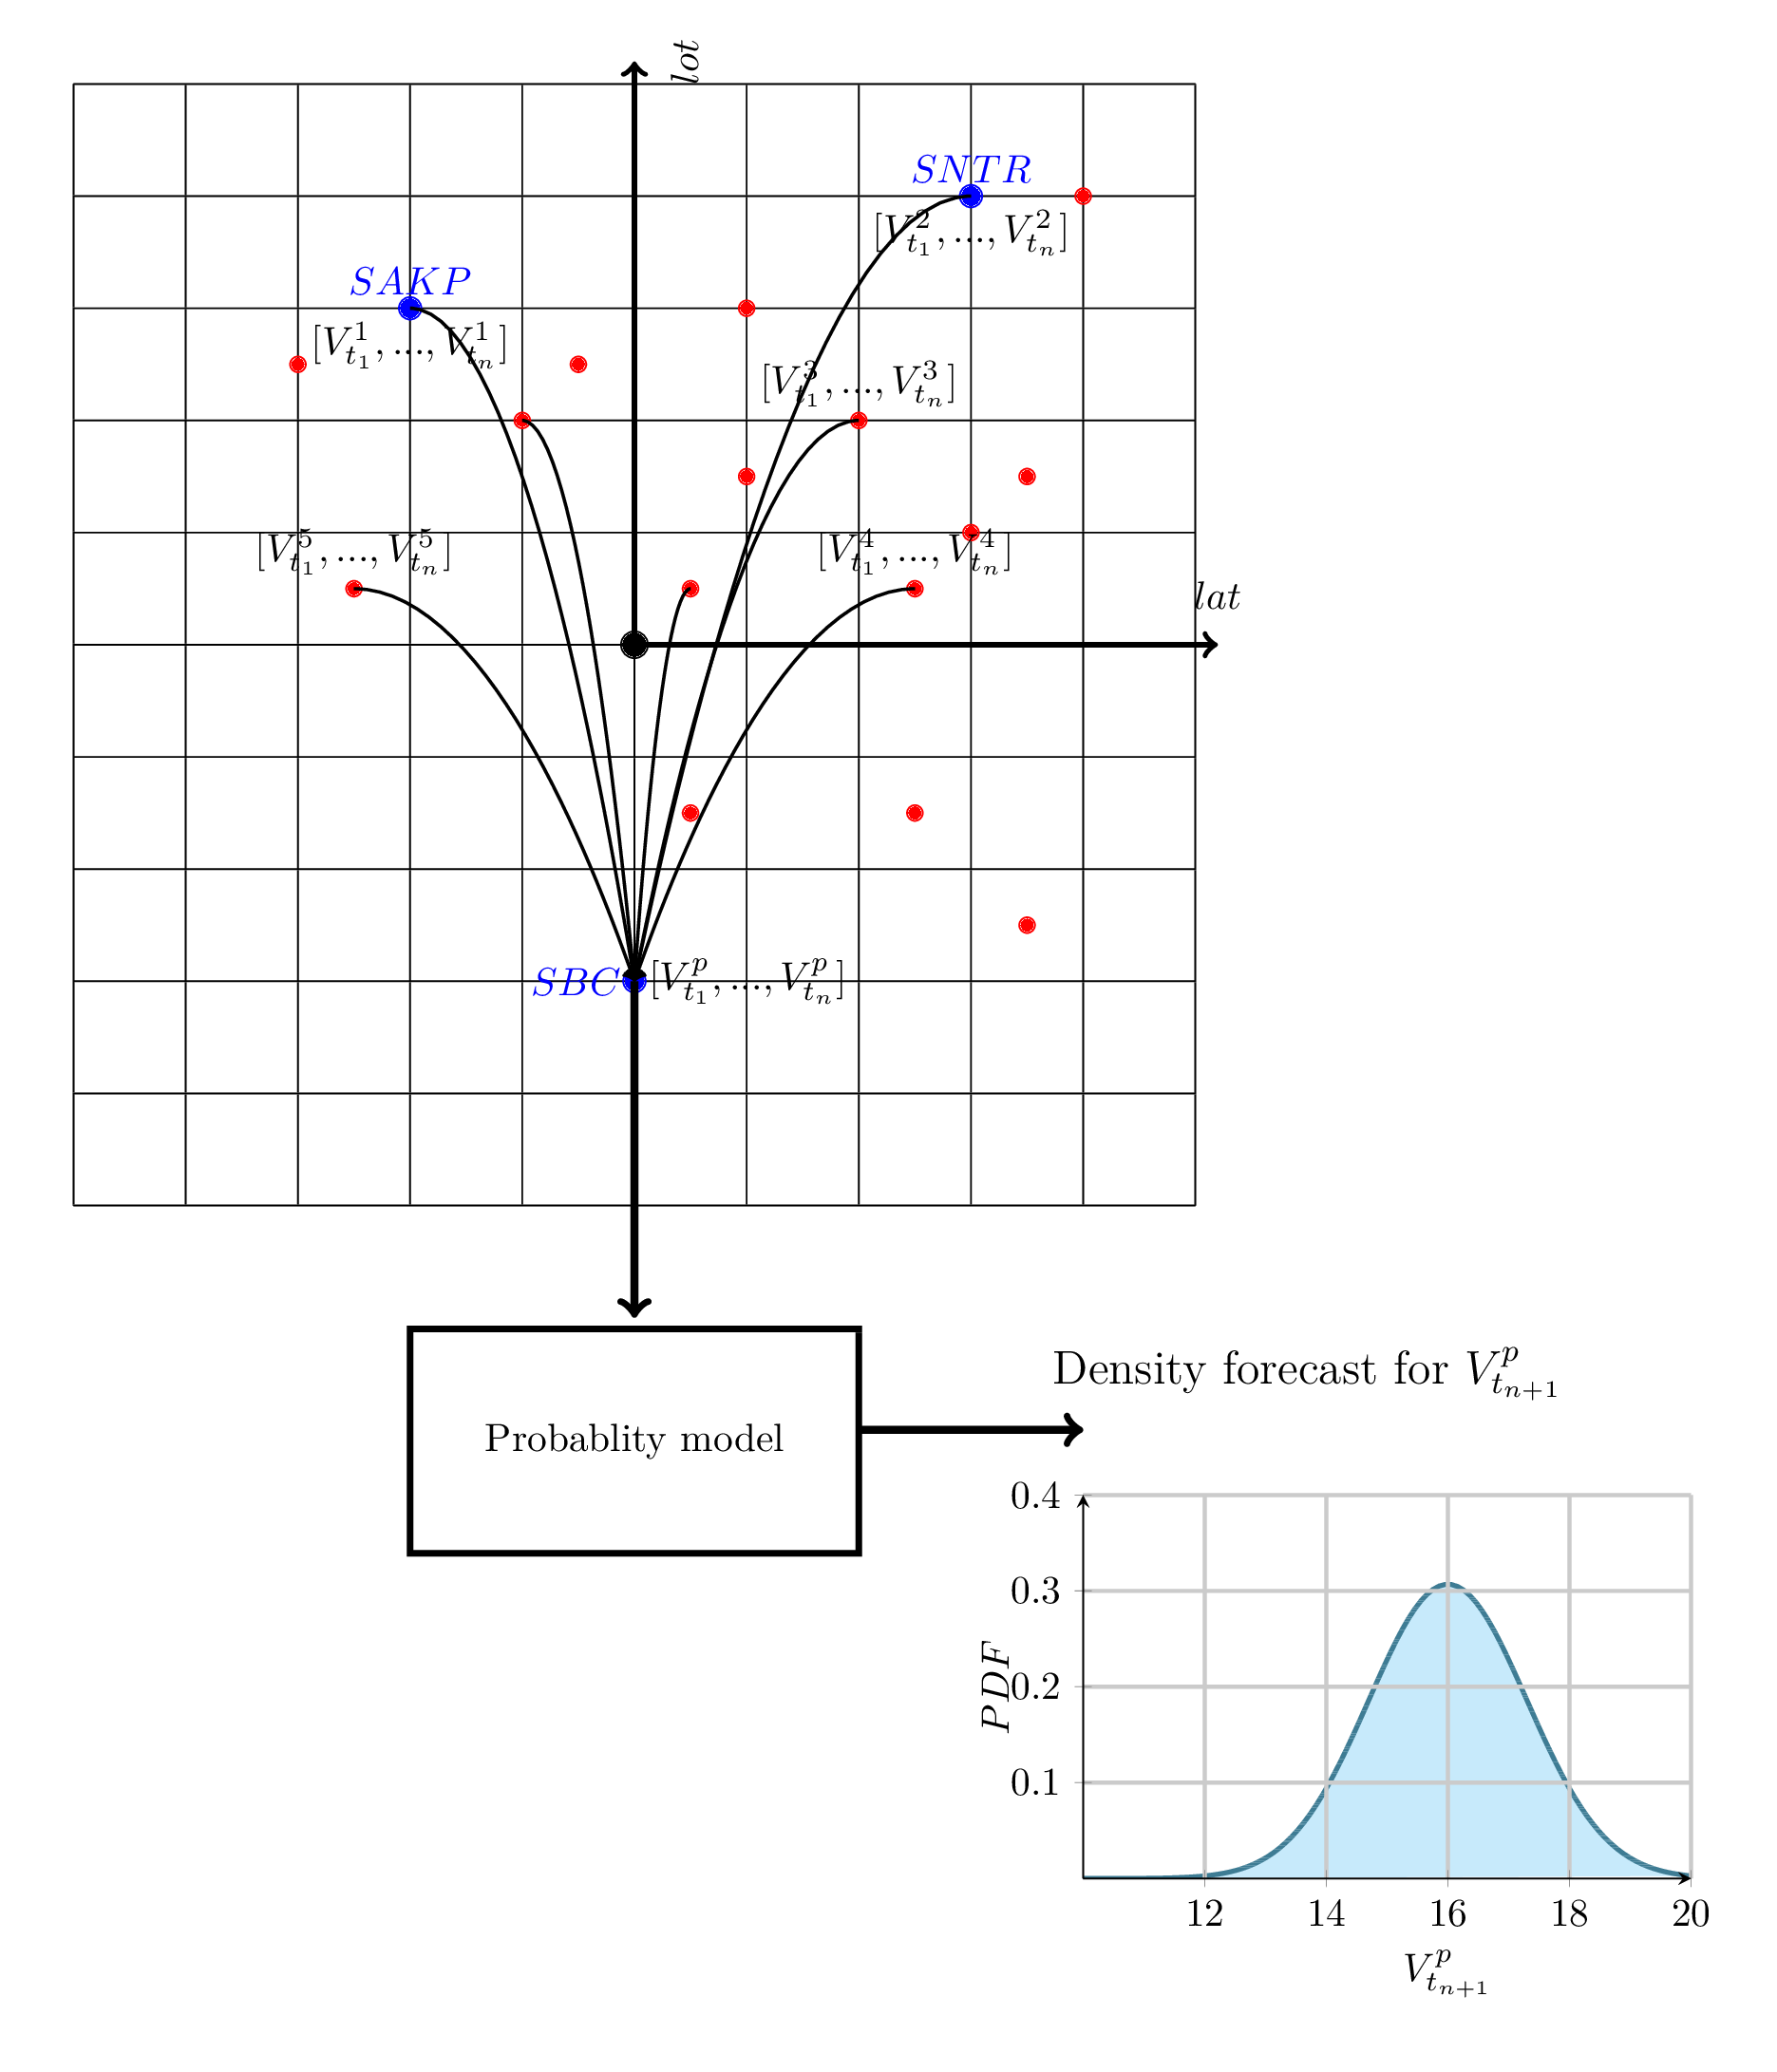
\includegraphics[height=1\textwidth, width=1\textwidth]{figures/general_system.png}
    \caption[General system]{General view of the system we aim to build. The red dots represent unreliable DYI sensors. Data from all the sensors is used in order to make prediction for one (SBC) of the LUBW-Stations (shown in blue). The prediction made is for some future moment \(t+1\) and it is on the basis of the past -- the values of all moments till \(t+1\) from all the stations. The prediction is generated in form of a probability distribution generated by the probabilistic regression model.}\label{fig:general}
  \end{figure}
\end{center}
\subsection{Probabilistic regression}\label{sec:prob-regression}
Based on training data, regression models make a real valued prediction given an input data point. Each time a prediction is made, one would desire to have a certain measurement for the uncertainty of the prediction. If this is the case and the prediction is given in a form of some distribution, we say that the forecast is probabilistic. This quantification of the uncertainty allows for optimal decision making. Models that produce such probabilistic forecasts have gained recent popularity in areas such as meteorology, seismology and economics. In \refsec{sec:related-work} we look at concrete cases where probabilistic regression is applied.

Probability forecasts are well established for classification models. Through the use of a soft-max layer, first introduced in~\cite{denker1990}, neural networks can assign each class they recognize a certain probability. This thesis is centered, however, around probabilistic regression models. \emph{Probabilistic regression models} produce a probability distribution as their prediction rather than a point estimate. One can then draw samples from this distribution, make statements about the drawn samples and reason about the nature of the possible values that could be predicted. Illustration of this is given in \reffig{fig:pred-dist-draws}. Another way of thinking about probability forecasts is that they define a certain region where the predicted value can fall within. The region is defined in form of a probability distribution. The model tells us then what is the probability of each point within the region to be a predicted value given the input of the model. We say that the model describes the conditional probability of the output given the input (more details in \refsec{sec:prob-modeling}). \reffig{fig:prob-regression} illustrates these considerations about probabilistic regression models. We also give \refdef{def:prob-for} so that we can reference it later in the thesis.
\begin{center}
  \begin{figure}[H]
    \centering
    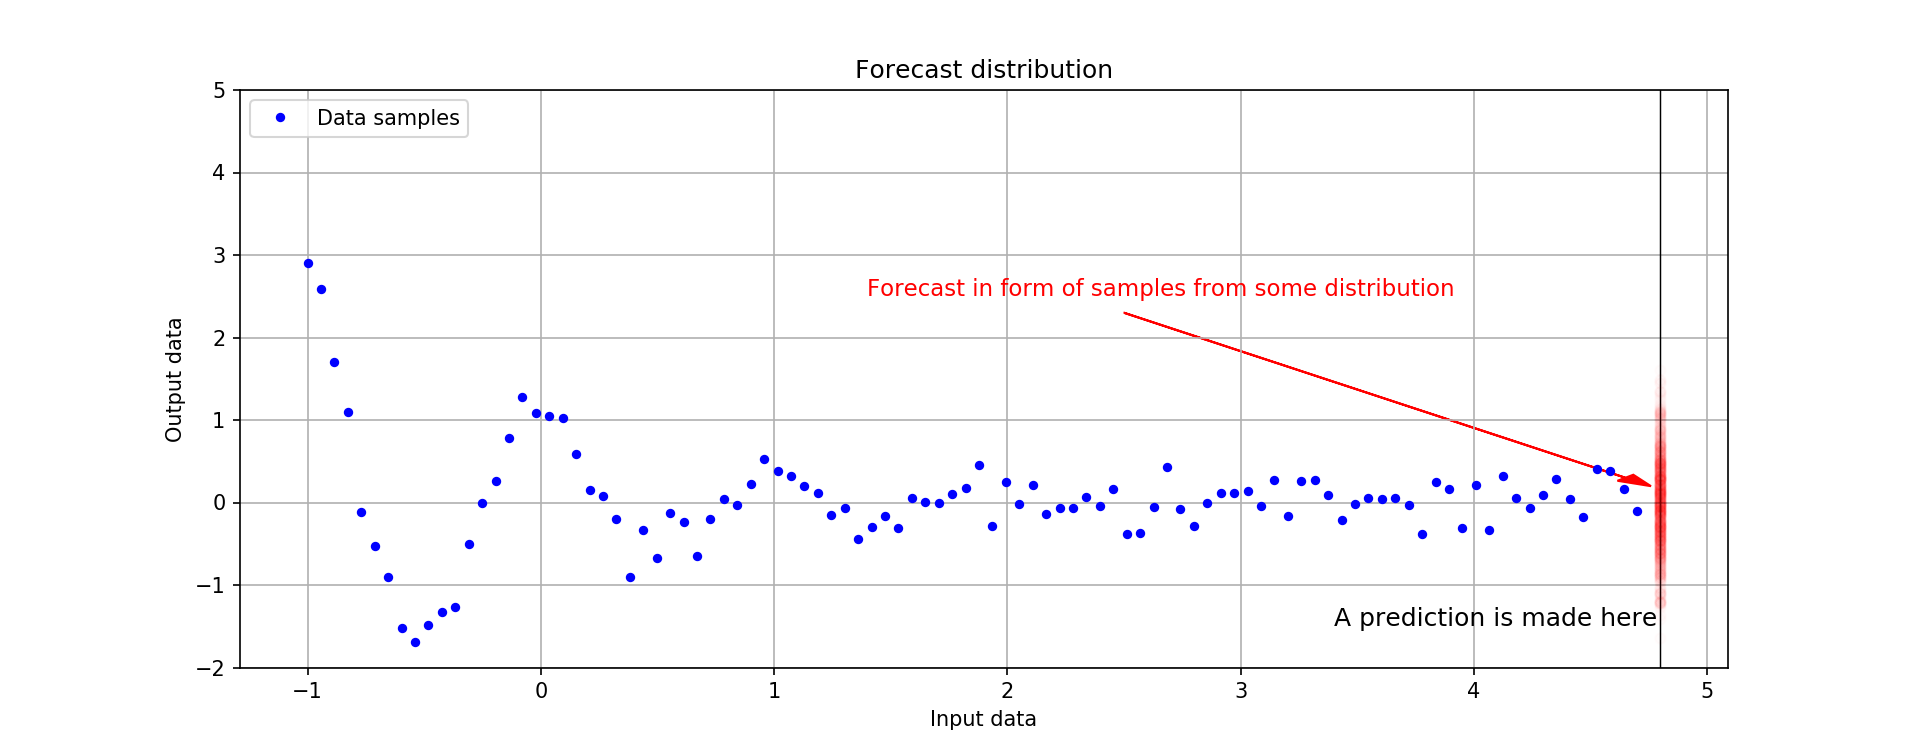
\includegraphics[height=0.5\textwidth, width=1.0\textwidth]{figures/forecast.png}
    \caption[Forecast sample draws]{Illustration of what samples from forecast can look like. The blue dots are observations. On their basis a prediction is made. The red dots are drawn samples from the predicted distribution. We can see that those are concentrated near the most probable value of the observation at this place.}\label{fig:pred-dist-draws}
  \end{figure}
\end{center}
\vfill
\begin{figure}[ht]
  \centering
  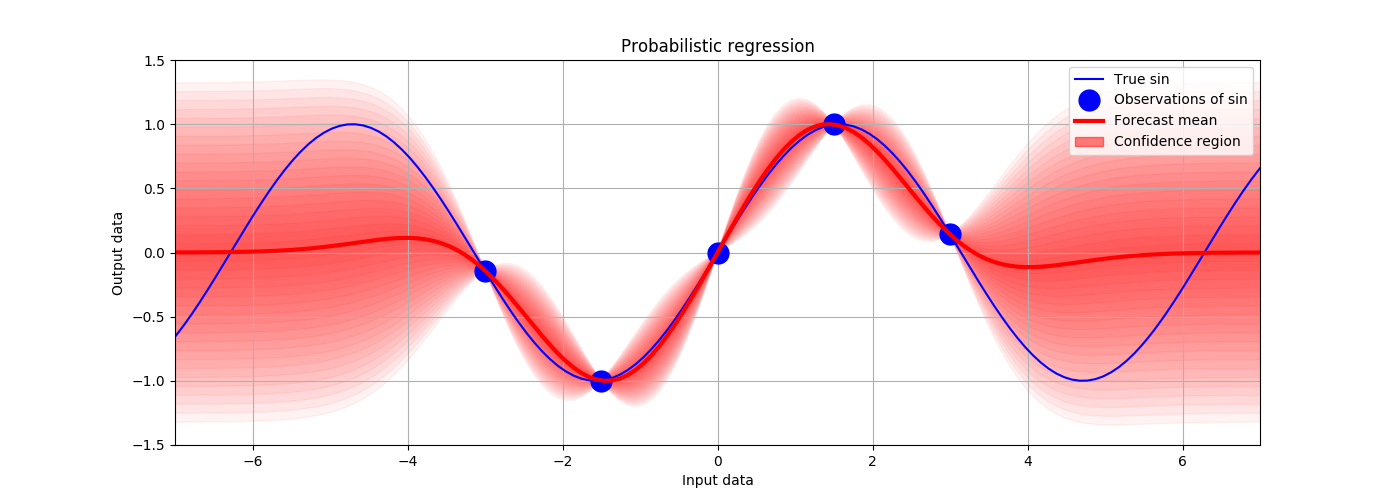
\includegraphics[height=0.5\textwidth, width=1\textwidth]{figures/probabilistic_regression.png}
  \caption[Probabilistic regression example model]{A probabilistic regression model (in red) that tries to model the \(\sin\)-function (in blue). The big blue circles are the observations of the function that the models becomes as training set. On the basis of those observations we construct a probabilistic model that can evaluate the whole input space. The model knows about the given observations of the modeled function so it predicts their values with high certainty. The places where there is no observed data, however, the model cannot make precise prediction and the distribution is wider. We notice, however, that true value of the function lies in the distribution so in sense the model predicts the function somewhat accurately.}\label{fig:prob-regression}
\end{figure}
\vspace{-2cm}
\begin{definition}{Probabilistic forecast:}\label{def:prob-for}
  Output of a probabilistic regression model for a single datapoint where the output represents some probability distribution. The distribution determines the probability of each point in space to be the regression value for the given considered input of the model. The distribution can be represented through certain amount of samples drawn from it, its density function or its cumulative distribution function. In the thesis we use probabilistic forecast, predicted distribution, distribution forecast, predictive distribution and forecast interchangeably.
\end{definition}
\vfill

Predicting distributions requires some consideration by the evaluation of the predictive capabilities of the considered model. When it comes to point estimates, one can simply measure the distance between the predicted and the realized value. Comparing a distribution with a single value, however, is not so straight forward. \reffig{fig:point-vs-dist} illustrates the apparent difference between point estimate and distribution prediction and how can one can reason much more, if a distribution for the prediction is present. In our evaluation of the models we employ the use of \emph{proper scoring rules}. A detailed look on the subject is given in~\cite{rafteryg2007}. The proper scoring rules can measure the error between a predicted probability distribution and a realized observation. We give more details on the proper scoring rules in \refsec{sec:proper-scoring-rules}.
\begin{center}
  \begin{figure}[H]
    \centering
    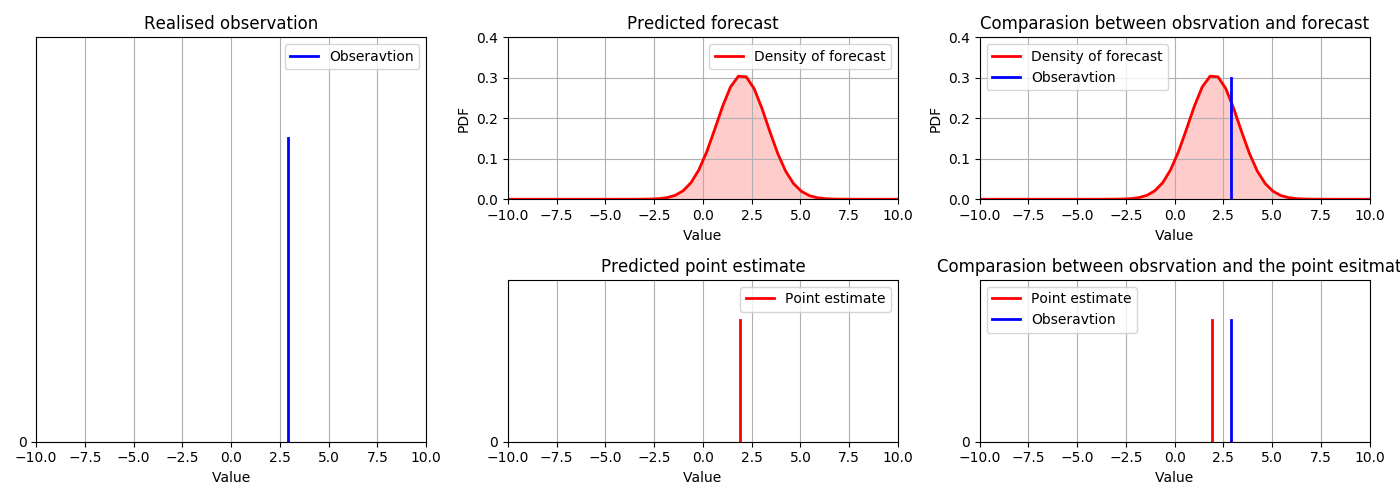
\includegraphics[height=0.5\textwidth, width=1.0\textwidth]{figures/distribution_point.png}
    \caption[Point estimate and distribution forecast]{The left most graph shows actual observation that is to be predicted. In the middle there are two prediction made by two different models -- a probabilistic forecast (on the top) and point estimate (on the bottom). With the right graphs one can clearly see how there is not a whole lot to compare between the point estimate and the observation other than the distance between the two. With the probability forecast, however, we can evaluate where and how exactly fits the observation in the predicted distribution.}\label{fig:point-vs-dist}
  \end{figure}
\end{center}
\vfill

The quality of probabilistic forecasts have two important characteristics:
\begin{itemize}
\item Calibration -- a measure of the compatibility between the forecast and the observation. This property depends both on the observation and on the forecast. The forecast is assumed to be in a form of a probability distribution.
\item Sharpness -- a measure of the concentration of the forecast. This property is purely based on the predicted forecast. The forecast is again some predicted probability distribution.
\end{itemize}
We look at the two properties in details in \refsec{sec:prob-modeling}.

The statistical framework for inferring probability distributions is \emph{Bayesian Inference}. A good theoretical and practical overview of Bayesian inference can be found in~\cite{tipping2004}. In Bayesian inference \emph{Bayes theorem} (see~\cite{bayes63}) plays a central role in determining the probability for a hypothesis given some evidence. Bayesian inference takes into consideration our prior beliefs about the nature of some data and then combines these beliefs with the actual observed data (denoted as \emph{evidence}) and generates \emph{posterior} probability about the values of the output. We discuss Bayesian reasoning in \refsec{sec:bayesian-inference}.
\subsection{Data}\label{sec:data}
The air pollution data that we use was recorded by a network of sensors over one year period for the year of 2017. As previously stated, the data comes from two different types from sources.
\begin{itemize}
\item \href{https://www.lubw.baden-wuerttemberg.de/startseite}{LU-BW} (Landesanstalt für Umwelt, Messungen und Naturschutz Baden-Württemberg) -- Organisation whose activities include air measurements and high quality sensors deployment. LUBW has gathered data from three high quality sensors in Stuttgart for the year 2017. The data is to be used for research proposes only and is not publicly available.
\item \href{https://luftdaten.info/}{luftdaten.info} -- a public network of sensors where everyone can provide data from sensor from certain type. There we can find air pollution data from \emph{sds011}-sensors (see~\cite{sds011}  for specifications). Those are cheap DIY sensors and give no guarantees for the quality of the measured data. Measurements of wide networks of such sensors are publicly available under~\cite{luftdaten}.
\end{itemize}
All of the sensors measure two types of air pollution data. The different naming of these values relates to the size of the measured particles. The two data types are:
\begin{itemize}
\item \emph{PM2.5} -- Particular matter up to 2.5 micrometers.
\item \emph{PM10} -- Particular matter up to 10 micrometers.
\end{itemize}
We found that those values are highly correlated -- correlation of about 0.95 on average (see \refsec{sec:preprop-meth} and \refapp{app:a} for details). For this reason the built models use either PM2.5 or PM10. That is, with PM2.5 data of all other sensors, we predict the PM2.5 values of a particular sensor or respectively with PM10 data we predict PM10 values.

The format of the data coming straight from the networks was not convenient for direct training of the models. The sensors from \emph{luftdaten} provide measurements for each minute over the whole year while the ones of LUBW integrate their measurements over thirty minutes. Because of this inconsistency we had to ``synchronize'' the both data sources in order to produce the final data sets. We've also found numerous problems with the data from \emph{luftdaten}. Some of them are:
\begin{itemize}
\item Not all sensors are located around Stuttgart.
\item Some of the sensors have a lot of missing days without measurements.
\item Some of the sensors have missing measurement in random minutes of the day.
\end{itemize}
The raw data was extensively preprocessed with different techniques. We explain the preprocessing of the data in \refsec{sec:prep-data}.
\subsection{Models}\label{sec:models}
The models of interest that we are going to look at are \emph{Bayesian Neural Networks} (\emph{BNNs}, see \refsec{sec:bnn}) and \emph{Mixture Density networks} (\emph{MDNs}, see \refsec{sec:mdn}). Here we give brief overview of the both models and we discuss them in detail in the respective sections.

BNNs are relatively new type of model proposed in the 1990s and studied in depth in~\cite{mackay1992} and~\cite{neal1996}.~\cite{gal2016} provides a general survey and a study on the uncertainty quantification in deep learning. More recently BNNs have seen a surge in popularity as they combine Neural Networks with Probabilistic Models. The inferred distributions over their parameters allows them to offer a probability distributions for their estimates. This makes BNNs attractive to the machine learning community as those properties give them robustness to over-fitting and the ability to learn from small datasets. These properties of the BNNs are well documented in~\cite{neal1996}. BNNs place prior distribution on their weights. The posterior distributions are estimated either by variational inference (\cite{blundell2015},~\cite{paisley2012}) or by sampling techniques (\cite{vehtari2000}). In our work we use variational inference with \emph{Kullback-Leibler divergence} and give details about the method in \refsec{sec:var-inference}.

With MDNs we hope to construct a model similar to an infinite mixture of Gaussian experts, proposed in~\cite{rasmussen2002}. The mixture of Gaussian experts is a combination of several Gaussian process regression models and a gating network. Given an example data point the gating network assigns certain probabilities for each of the Gaussian process models. On their turn they generate several probability distributions which are weighted with the probabilities from the gating networks. The end result again is a probability distributions given by the sum of the individual ones. MDNs model this by creating a single network that not only outputs weights for the individual mixture components but also their parameters. MDNs are very similar to standard Neural Networks with the only difference being that final layer is mapped to a mixture of distributions. In our case the mixture model is a weighted sum of Gaussian distributions. MDNs produce especially good results when the input data is such that a single input can correspond to multiple output values. In those cases, the predicted distribution models the corresponding output values by giving some probability on each of them. We investigate what results one can get when this approach is used for simpler data. As MDNs are almost standard neural networks, they are trained with the standard \emph{backpropagation} method, described for example in~\cite{bertels2001}.

In order to have a baseline with which we can compare the built models we also construct a simple empirical model. The empirical modeling is a technique for making predictions about the values of some process based purely on empirical observations of past values of the process. In this cases there is no consideration of the input of the data but rather a simple looking at the past values of the output value. The past values of the predicted measurement are treated as samples from a random variable. We describe how we infer a probability distribution for a prediction in \refsec{sec:emp-impl}. Similar empirical models are commonly used for simple predictions of meteorological data. Examples of this approach can be found in~\cite{krueger2011} and~\cite{eden2015}.
\clearpage
\section{Related work}\label{sec:related-work}
Heterogeneous sensor networks are present in a lot of cases.~\cite{wu2007} examines the deployment and the control of the topology of heterogeneous wireless sensor networks.~\cite{katiyar2010} surveys a variety of clustering algorithms aimed at increasing the network's scalability by recognizing the sensors with similar energy requirements.~\cite{uplap2014} investigates the kinds of security threats that arise with the use of heterogeneous sensor networks. In the context of machine learning,~\cite{liu2017} tries to use deep learning techniques and adapt them to the settings of heterogeneous sensor data.

\cite{gneiting2014} has brought a lot of attention to probabilistic forecasting. When it comes to history,~\cite{stigler1975} describes the transition from point estimates to distribution prediction. Nowadays the technique is widely used in variety of cases as it is further developed (\cite{ehm2012}). Common areas where probabilistic forecasts are employed are whether and climate prediction. The approach is outlined in~\cite{collins2007}. There are also other diverse applications. ~\cite{krzysztofowic2001} looks how probabilistic models can be used for flood risk assessment,~\cite{timmermann2001} describes probabilistic models within the context of economic and financial risk management,~\cite{pinson2013} investigates the potential to make predictions about the availability of renewable energy resources. \cite{montgomery2012} shows how distribution forecasting can be even used to make statements about the outcome of elections.

The other focus of our work are BNNs. As models that tie Bayesian reasoning and neural networks together, they have also gained popularity. A good outline of neural networks and deep leaning can be found in \cite{schmidhuber2015}. \cite{vehtari2001} first gives a brief overview of the Bayesian approach to neural networks and then surveys different use cases assessing the performance. Fields like astrophysics \cite{bai2016} and particle physics \cite{bhat2015} also profit from the predictive capabilities of BNNs. As medicine is one of the fields that gets much of the attention of the machine learning research, \cite{kwon2017} applies BNNs in order to quantify the uncertainties and apply them in ischemic stroke lesion segmentation. BNNs are also continuing to be developed. \cite{fortunato2017} explores the Bayesian approach in Recurrent Neutral Networks developing \emph{Bayesian Recurrent Neural Networks}.

MDNs have also found popularity as an another alternative to combine neural networks with distribution forecast models. \cite{schittenkopf1998} uses MDNs as a general framework for identifying stochastic processes and apply them in modeling stock exchange index data. \cite{zen2014} brings MDNs to use in order to improve deep neural networks for acoustic modeling. MDNs have their own variant of recurrent models as described in \cite{miazhynskaia2003}. We like to note that MDNs have similar structure to other models such as \emph{Adaptive mixture of local experts} -- proposed by \cite{jacobs1991}) -- and \emph{Infinite Mixtures of Gaussian Process Experts} -- proposed by \cite{rasmussen2002}. MDNs, however, model the data differently. We explain the approach in \refsec{sec:mdn}.

The use of proper scoring rules is standard in probability forecast setting. \cite{jordan2017} discusses the \textbf{scoringRules} package for \emph{R}\footnote{Programming language} and its usage details by presenting case studies where proper scoring rules find application. \cite{clements2004} uses probability integral transform in order to evaluate the UK Monetary Policy Committee's inflation density forecasts. We describe probability integral transform in \refsec{sec:disp-sharp}.
% \cite{friederichs2012} deals specifically with verifying predicted probability distributions under the use of proper scoring rules.
\section{Probabilistic Modeling}\label{sec:prob-modeling}
\subsection{Bayesian regression modeling}\label{sec:bayesian-inference}
In a probabilistic modeling setting we aim to estimate the parameters of a given model by first defining some \emph{prior} on them. The prior distribution describes how likely values of the parameter are without considering any observed data. Then a \emph{conditional likelihood} for the output based on the parameters and the input data is defined. This probability distribution describes the probability of observing certain data given the parameters of the model. The assumption here is that that the model has generated the data. The two distributions are then combined in order to produce the final \emph{posterior} probability distribution on the parameters of the model. A good overview of Bayesian models can be found in \cite{mitchell97}. We can summarize:
\begin{itemize}
\item \textbf{Prior} -- uncertainty in form of probability distribution \emph{before} observing the data.
\item \textbf{Posterior} -- uncertainty in form of probability distribution \emph{after} observing the data.
\end{itemize}

Now we formally write down everything following the approach of \cite{gal2016}. Let
\begin{equation}
  X = \{x_1,\ldots , x_N\}, \forall i : x_i\in\mathbb{R}^M
\end{equation}
be the set of input data. The corresponding output is given by the set \(Y = \{y_1,\ldots , y_N\}\). The dataset can also be seen as tuples of feature vector \(x_i\) and an output value \(y_i\). We can then write the dataset as \(\{ (x_i,y_i)\}_{i=1}^N \). As we deal with regression models we assume that \(\forall i : y_{\text{i}}\in \mathbb{R}\) and there is some function \(f_{true}:X \rightarrow\mathbb{R}\) with \(f_{true}(x_i)=y_i, \forall i \in\{1,\ldots , n\}\). We want to find a model with appropriate parameters that is likely to have generated the data. In fact, through the choice of parameters, we want the observed data to be as probable as possible. We model the mapping function between \(X\) and \(Y\) through a separate function \(f_m(x; \omega)\) parameterized by \(\omega\). We want to find a ``good'' set of parameters \(\omega\) such that the function \(f(x;\omega)\) is \emph{likely} to have generated the output data. We define our prior believes about the parameters through the distribution \(p(\omega )\). The generalized likelihood distribution is then \(p(y|x, \omega)\). That is, how likely is output \(y\) given model parameters \(\omega\) and concrete input \(x\). Our assumption here is that the defined model generates the data. The output of a regression model is typically set to be a Gaussian likelihood: \(p(y|x,\omega)=\mathcal{N}(y; f_m(x;\omega), \tau^{-1}I)\) where \(\tau\) is the model precision. This can be interpreted as adding small amount of noise to the output as modeled in \cite{gal2016}.

We can now write out the posterior by using the Bayes' theorem:
\begin{equation}
  p(\omega|X,Y) = \frac{p(Y|X, \omega)p(\omega)}{p(Y|X)}
\end{equation}
This distribution describes the most likely model parameters given the observed data. If we draw parameters from this distribution, the observed data will be most likely. For prediction of new data point \(x^*\) we use
\begin{equation}
  p(y^{\text{*}}|x^{\text{*}},X,Y) = \displaystyle\int p(Y|X, \omega)p(\omega)d \omega
\end{equation}
This integration is called \emph{inference} (\cite{gal2016}). The quantity
\begin{equation}
  p(Y|X) = \displaystyle\int (Y|X, \omega)p( \omega )d \omega
\end{equation}
is called marginal likelihood or sometimes ``model evidence''. The first name comes from the fact that we are marginalizing the likelihood over \(\omega\). This factor is independent of the parameters so no matter how we choose them, it does not change. Marginalization plays central part in Bayesian modeling and in the prefect case we would want to marginalize over all possible parameter values \(\omega\) with respective weight \(p(\omega)\). In complex models this is not possible and we resort to approximations.

``Learning'' in this Bayesian setting boils down to finding the posterior distribution \(p(\omega |X, Y)\) over the parameters. In the general case this cannot be done analytically (a closed formula cannot be given) and thus one must attempt to approximate the distribution.

Inference provides us with the full probability distribution over the parameters and for that reason we are not dealing with point estimates of the parameters. By extension we can also provide some distribution when we evaluate the model on unseen data. In order to ``generate'' a sample from the resulting distribution for some unseen input data point \(x^*\) we first need to sample \(\omega_s\) from the parameter distribution and then evaluate the model \(f_e\) at point \(x^*\) parameterized by the drawn sample \(f_e(x^*; \omega_s)\).

The models that we consider next are nothing more than concrete choices for \(f_e\) and its parametrization.
\subsection{Bayesian Neural Networks}\label{sec:bnn}
\subsubsection{Neural networks}\label{sec:nn}
\noindent\emph{First we give brief overview of conventional neural networks.}

Neural networks (or artificial neural networks) are computing systems that model some arbitrary function through their structure and parameters. Neural networks consist of artificial neurons that have a certain number of inputs. They first compute a weighted linear sum of their inputs and then apply a non-linearity in form of \(\tanh\), logistic or other type of \emph{sigmoid} function. Several stacked neurons are considered a layer of a network. Several consecutive layers where the output of one layer is the input of the next are considered a \emph{neural network}.

Formally the neural network is nothing more than a parameterized function with specific structure that allows it to estimate almost every possible function when given the right parameters. Let \(W_i \in \mathbb{R}^{A_i \times B_i }\) and \(b_i\in\mathbb{R}^{B_i}\) be weight matrices and biases respectively and let \(o_i\in\mathbb{R}^{B_i}\) denote the output of the \(i^\text{th}\) layer of the network. For an input \(x\in \mathbb{R}^{A_1}\) we then have:
\begin{align}
  o_{1} &= \tanh((W_{1}x) + b_{1}) \\
  o_{2} &= \tanh((W_{2}o_1) + b_{2}) \\
        &\vdots
\end{align}
In general, for a network with \(m\) layers where the \(m^{\text{th}}\) layer is the output layer, the outputs of the individual layers can be given as:
\begin{align}
  \label{eq:nn-ouput}
  o_{i+1}  &= \tanh((W_{i+1}o_i) + b_{i+1}) \\
  o_m     &= (W_{m}o_{m-1}) + b_{m}
\end{align}
where \(o_m \) is the final output of the network. The forward evaluation of the network is just a cascade of applications of liner functions in form of a matrix multiplication and addition of bias term followed up by an application of some non-linear function. For sake of simplicity let us collapse the notation of the output of the network to a single function of the input \(x\) and the collection of parameters (weight matrices and bias-terms) to \(\Omega\). The evaluation of the network can be given with
\begin{equation}
  o_m = f_{net}(x; \Omega)
\end{equation}
A visual representation of a neural network is given in \reffig{fig:nn}.
\begin{center}
  \begin{figure}[H]
    \centering
    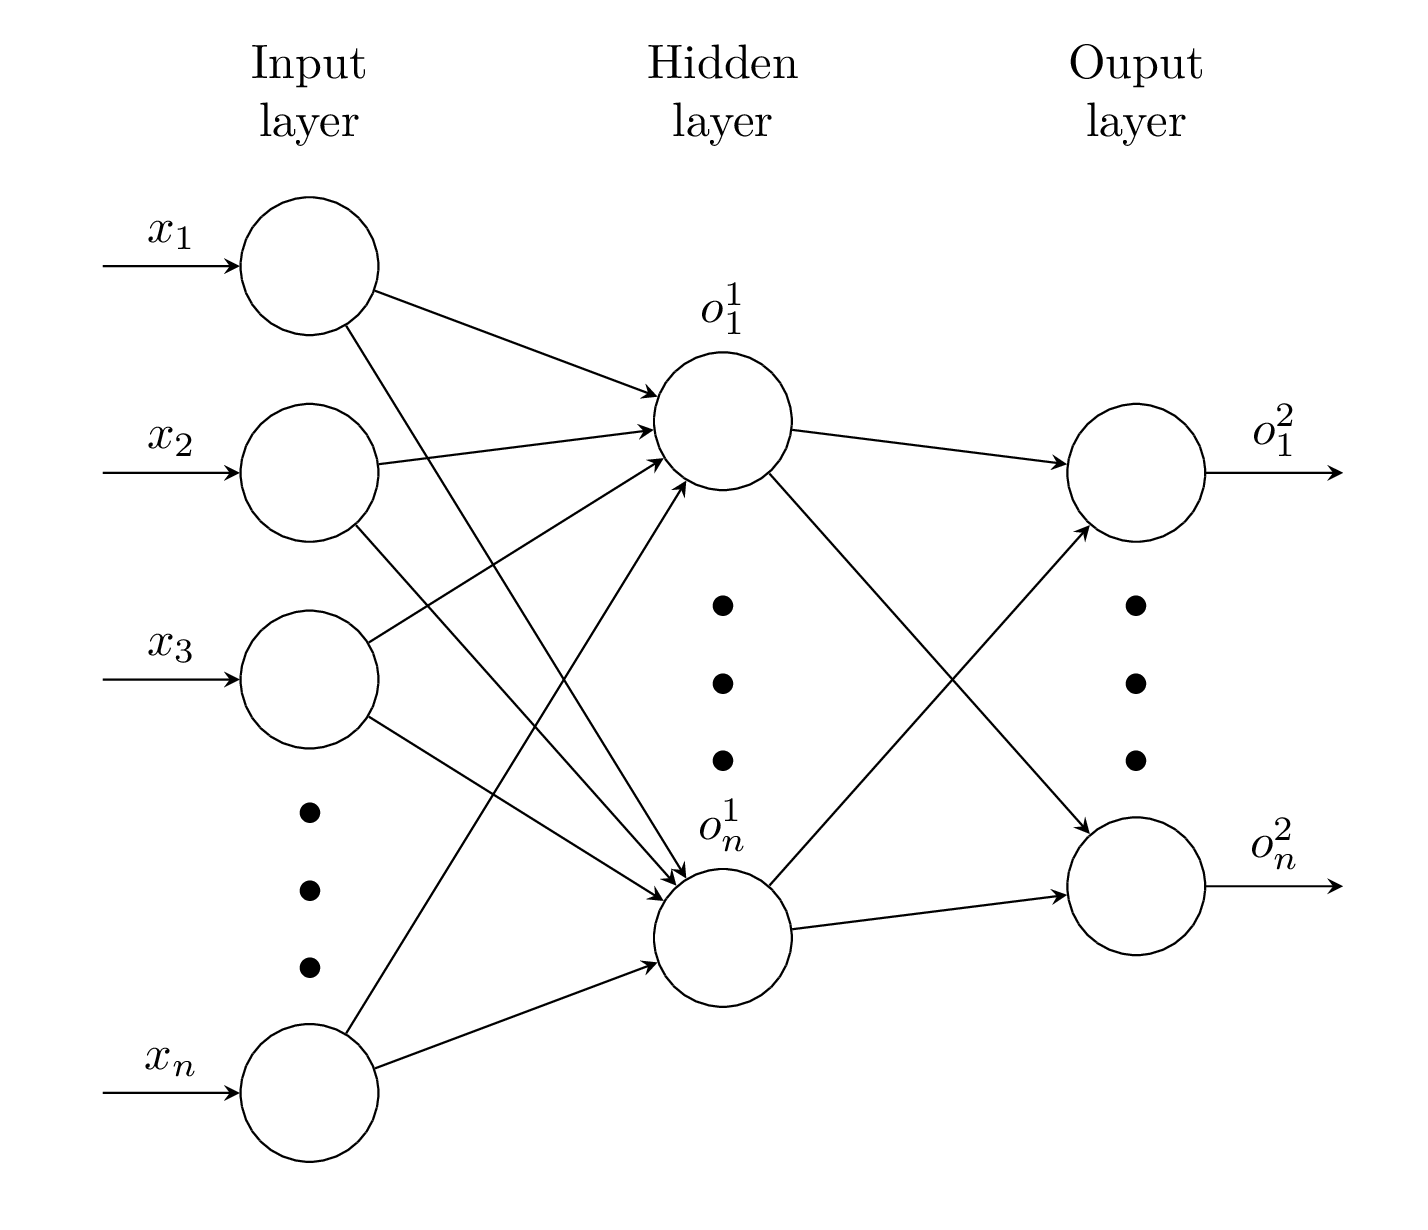
\includegraphics[height=0.65\textwidth, width=0.8\textwidth]{figures/nn.png}
    \caption[Neural Network Schematic]{A schematic of a neural network with one hidden layer. The circles represent individual neurons. The data flows from left to right as the neurons sum up their weighted inputs, apply non-linearity and pass their outputs to the neurons in the next layer.}\label{fig:nn}
  \end{figure}
\end{center}

In order to be useful we have to ``teach'' the neural network our desired mapping. As in previous section we have a set of input data \(X = \{x_1,\ldots , x_N\}, \forall i : x_i\in\mathbb{R}^M\) and the corresponding output for each \(x_i\) is contained in the set for the output data \(Y = \{y_1,\ldots ,y_N\}, \forall i : y_i\in\mathbb{R}\). Ideally we would want the following to hold for the neural network
\begin{equation}
  f_{net}(x_i;\Omega) = y_i
\end{equation}
In other words, the network has \emph{learned} the exact mapping between \(X\) and \(Y\) and can predict the output value based on the input one. This is done by choosing appropriate parameter set \(\Omega\). In general, finding parameters realising the exact mapping will not be possible but we want to at least approximate this case. This leads us naturally to a definition of measurement of just how wrong the network is. We call this quantity \emph{error function} (also called \emph{loss function}). The error function is a function of the parameter space and it gets closer to zero as the parameters define a network that better models the data. There are lot of possible choices for loss function but the most common is the \emph{squared error difference}:
\begin{equation}
  E(\omega) =  \sum_{i=0}^N (f_{net}(x_i;\omega) - y_i)^2
\end{equation}
where \(\omega\) is some choice for the parameters for the networks, namely \(m\) weight matrices and \(m\) bias terms for network with \(m\) layers. The squared error difference is a simple sum of all differences between predicted by the network value and the actual value. If the defined function is zero, the network essentially predicts all values correctly. Minimizing this \emph{error function} is what we call \emph{learning} the data or \emph{training} the network. The actual method trough which learning occurs is \emph{backpropagation}. This involves calculating the derivatives of the loss function with the respect to each parameters of the network \(\frac{\partial E}{\partial W_i }\). The corresponding parameters are then updated through some gradient descent technique. An overview of different gradient descent techniques can be found in~\cite{ruder2016}. Some state of the art optimization methods are \emph{LM-BFGS} (Limited Memory Broyden–Fletcher–Goldfarb–Shanno algorithm, see \cite{byrd1995}), Adam optimization algorithm (see~\cite{kingma2014}) and \emph{SGD} (Stochastic gradient descent, see~\cite{robbins1951}). To note is that the last motioned method -- the SGD -- does not calculate the gradient of the loss function using all of the training examples rather it uses only a small subset of the training set.

We would like to note that neural networks are considered universal function approximators. This means that given enough complexity of their structure, they can model arbitrary non-linear functions. A prove for this statement is provided in~\cite{hornik1989}.
\subsubsection{Neural networks in Bayesian settings}\label{sec:nn-in-bayesian}
\noindent\emph{In this section we focus specifically on Bayesian neural networks}.

BNNs place a prior distribution over the parameters of a neural network. As described in previous section, once we have distributions on the parameters of a model, we have effectively defined a distribution over functions. Each time when we draw a sample from the parameter space, we have defined a ``new'' function that models the given data. In this sense, we have sampled a new function from some distribution. Usually, for given weight matrix \(W_i\) and bias term \(b_i\) in layer \(i\) of the network, BNNs place standard Gaussian prior distributions over the matrices, \(p(W_i)=\mathcal{N}(0,I)\) and a point estimate for the \(b_{\text{i}}\) is assumed. In this work, however, the standard prior is also placed on the bias vectors so we define the distributions \(p(b_i)=\mathcal{N}(0,I)\).

The basic structure of the BNNs is the same as the one of regular neural networks. For this reason we will use the notations from the previous section. The output of the network for a given input \(x\) and parameters \(\omega\) is
\begin{equation}
  f_{net}(x;\omega)
\end{equation}
We have now defined what the basic structure of our considered model is (a neural network) and we know what the priors over the parameters of the model are. As in the previous section we now define a likelihood for each data point. We consider a set of data \(\{(x_i, y_i), i\in\{1,\ldots ,n\} \}\) where each data point has some features \(x_i\in\mathbb{R}^M\) of dimension \(M\) and real valued output \(y_i\in\mathcal{R}\). We define the likelihood for the BNNs as:
\begin{equation}
  p(y_i|\Omega, x_i, \sigma^2) = \mathcal{N}(y_i |f_{net}(x_i;\omega), \sigma^2)
\end{equation}
where \(\sigma^{\text{2}}\) is again some known small variance that can be considered as ``noise'' of the output (\cite{gal2016}).

With this overview we can make several general statements about the BNNn. A BNN is a probability model that utilizes a neural network as universal function approximator. The distributions on the network's parameter allow it to generate a distributional output rather than a point estimate. This the exact same Bayesian setting as described in \refsec{sec:bayesian-inference}. 

The final piece of having some useful model is to have notion what ``learning'' means in the case of BNNs. As this is a Bayesian probability model we have to find the posterior distribution over the parameters based on the example data:
\begin{equation}
  p(\omega|Y,X)=\frac{p(Y|X,\omega)p(\omega)}{p(Y|X)}
\end{equation}
This distribution describes the most likely parameters given the example data. Direct computation of the posterior is not possible for networks of any practical sizes. The problems come from the term in the denominator as it involves integrating over the whole parameter space:
\begin{equation}
  p(Y|X) = \int_{\Omega} p(Y|\omega , X)p(\omega|X)d \omega
\end{equation}
In the next section we describe a technique that aims to estimate the posterior distribution without actually having to approximate the above integral. Once we have the posterior distribution (or a sufficient estimate of it) we could use it to produce the predicted distribution for unseen data samples. This is done through \emph{inference} as described in \refsec{sec:bayesian-inference}.
\subsubsection{Variational inference and Kullback-Leibler divergence}\label{sec:var-inference}
As previously stated, it is impractical to compute the full posterior. In fact, the true posterior is intractable and cannot be evaluated analytically. We therefore rely on an estimation technique that transforms the Bayesian inference into an optimization problem -- \emph{variational inference} (first proposed in~\cite{jordan1999}, see an overview in \cite{blei2016}, a detailed look in~\cite{fox2012}). We define a \emph{variational} distribution \(q_{\theta}(\omega)\), parameterized by \(\theta \). We assume that this distribution is easy to evaluate. Furthermore we would really like this distribution to be able to approximate other distributions based on the choice of parameters \(\theta\). If those assumptions are met, we then try to choose such parameters for \(q_{\theta}(\omega)\) that it maximally resembles the posterior \(p(\omega|Y,X)\). For that we also need some measure between two distributions that gives us how ``similar'' they are. This is slightly analogous to the choice of loss function that is to be minimized. In this case we use the \emph{Kullback–Leibler} (\emph{KL}) divergence proposed by~\cite{kullback1951}. KL is defined as
\begin{equation}
  KL(q_{\theta}(\omega), p(\omega | X, Y)) = \int q_{\theta}(\omega) \log \frac{q_{\theta}(\omega)}{p(\omega | X, Y)}d\omega 
\end{equation}
KL is a measure of how one probability distributions differs from another. A Kullback–Leibler divergence of \(0\) implies the two distributions are identical. KL divergence does not have a maximum value as it is unbounded. We aim to minimize this function with respect to \(\theta\). Our problem then becomes:
\begin{align}
  \theta^* &= \underset{\theta}{\arg\min} \,  KL(q_{\theta}(\omega), p(\omega | X, Y))\\
           &= \underset{\theta}{\arg\min}\, \int q_{\theta}(\omega) \log \frac{q_{\theta}(\omega)}{p(\omega | X, Y)}d\omega \\
           & = \underset{\theta}{\arg\min}\,  KL(q_{\theta}(\omega), p(\omega)) - \mathbb{E}_{q_{\theta}(\omega)}[\log\, p(Y|w)]
\end{align}
The last cost function is known as the \emph{variational free energy} (\cite{neal1998},\cite{blundell2015}) or as the \emph{expected lower bound} (\cite{fox2012},~\cite{saul1996}). Thus the function that we want to optimize is
\begin{equation}
  \mathcal{L}(\theta, Y) = KL(q_{\theta}(\omega)||p(\theta)) + \mathbb{E}_{q_{\theta}(\omega)}[\log(p(Y|\omega))]
\end{equation}
This loss function is a sum of a data-dependent part and a prior-dependent part. The function embodies a trade-off between satisfying the complexity of the data \(X \text{ and } Y \) and satisfying the simplicity of the prior \(p(\omega)\)(see \cite{blundell2015} for the derivation of the function).

Gradient calculation of this function is not a trivial task. As we use standard Gaussian priors on the parameter \(\omega\), the first term in the function (the KL divergence) is traceable and analytically solvable (\cite{paisley2012}). The other term, however, is not that well behaved. Several methods have been proposed to optimize the function with backpropagation techniques. The concrete implementation that we (\cite{edward}) use, utilizes either \emph{Stochastic Gradient Vitiation Bayes} (\emph{SGVB}) as described in \cite{kingma2013} or the method described in \cite{paisley2012}. 

\emph{We now give a brief overview of SGVB}. For the approximation of the posterior \(q_{\theta}(\omega)\) we reparameterize the random variable \(z \sim q_{\theta}(\omega)\) by the use of some differential transformation \(g_{\omega}(\epsilon , x)\) and a noise variable \(\epsilon\).
\begin{equation}
  z =  g_{\omega}(\epsilon , x), \quad \epsilon \sim p(\epsilon)
\end{equation}
With those definitions we can now estimate the expected value of some function \(f(x)\) with respect to \(q_{\theta}(\omega)\):
\begin{equation}
  \mathbb{E}_{q_{\theta}(\omega)}[f(x)] = \mathbb[f(g_{\omega}(\epsilon , x))] \simeq \frac{1}{L}\sum_{l=1}^L f(g_{\omega}(\epsilon^{(l)} , x))
\end{equation}
We can apply this technique to our cost function and we get a tractable and a differentiable estimate of it
\begin{equation}
  \mathcal{L}(\theta, Y) \simeq \mathcal{L}(\theta,Y)^E = KL(q_{\theta}(\omega)||p_{\theta}(z))  + \frac{1}{L}\sum_{l=1}^L(\log(p_{\theta}(x|\omega)))
\end{equation}
Now that we have a function for which the gradients can be given analytically, we can optimize it with respect to the parameter \(\theta\). This is done typically through Stochastic Gradient Descent (see \refsec{sec:nn}). In this case we do not calculate the loss on the whole dataset but rather on s sub-sample of it. Let say we take \(M\) datapoints from dataset with \(N\) datapoints. We then essentially are making the estimate:
\begin{equation}
  \mathcal{L}(\theta, Y) \simeq \mathcal{L}(\theta, Y^M)^E_M = \frac{N}{M}  \sum_{i=1}^{M}\mathcal{L}(\theta, y_i)^E
\end{equation}
It is known that SGD leads to faster convergence with less computations (\cite{robbins1951}). It is also proven and observed (\cite{shapiro1996}) that SGD converges to the result of regular gradient descent. For those reasons, the usage of SGD is almost always preferable.

There is also a somewhat simpler approach of estimating the gradient of the loss function as described in~\cite{paisley2012}. Under some regularity conditions, a gradient of the form \(\nabla_{\theta}\mathbb{E}_qf \) where \(f \) is some untraceable function, \(q\) is some distribution and we take the gradient with respect to \(\theta\), can be rewritten as:
\begin{equation}
  \nabla_{\theta}\mathbb{E}_qf(\theta) = \int_{\theta} f(\theta)q(\theta) \nabla_{\theta}\ln(q(\theta)) d\theta
\end{equation}
Details on how this equation is derived can be found in~\cite{paisley2012}. The integral can then be estimated through Monte Carlo integration (\cite{hammersley1964}). This approach can be used to replace the \(\mathbb{E}_{q_{\theta}(\omega)}[\log(p(Y|\omega))]\) in the cost function. We can then again apply stochastic gradient descent in order to spare some computations and accelerate convergence. For more detail on the method see~\cite{paisley2012}.

Other techniques for posterior estimation rely on sampling from the posterior. This can be done for example by \emph{Gibbs sampling} (\cite{geman1984}), \emph{Metropolis-Hastings} (\cite{metropolis1953}, \cite{hastings1970}) or \emph{Hybrid Monte Carlo} (\cite{duane1987}). These are all so called \emph{Markov Chain Monte Carlo} (\emph{MCMC}) methods and are popular techniques for sampling from some posterior distribution. We, however, do not consider them here.
\subsection{Mixture Density Networks}\label{sec:mdn}
\emph{In this section we describe the theoretical background of our second considered model -- mixture density networks.}

We first explain the MDNs' approach in modeling the data. MDNs try to describe each data point \((x,y)\in X\times Y\) with a feature vector \(x\in\mathbb{R}^R\) and a value \(y\in\mathbb{R}\) directly through some mixture model.
\begin{equation}
  p(y|x)=\sum_{m=1}^M \alpha_m(x)\phi_m(y|x)
\end{equation}
where \(M\) is the number of mixture components and \(\phi_m(y|x)\) is the conditional density of the \(m^{th}\) kernel. The parameters (or weights) \(\alpha_m(x)\) are called \emph{mixing coefficients} (\cite{bishop1994}). To note is that everything in the model depends on the concrete input data \(x\). In this sense the parameters for the mixture change for every data point. We choose mixture of Gaussians as with appropriate weights it can model any arbitrary distribution. This means that theoretically MDNs with Gaussian mixture can be universal distribution estimators Similar to regular neural networks which are universal real valued function estimators. Thus all of the density functions become:
\begin{equation}
  \phi_m(y|x) = \frac{1}{2\pi^{c/2}\sigma_m(x)^c}\exp\{-\frac{\left\lVert y - \mu_m(x) \right\rVert^2}{2\sigma_m(x)^2}\}
\end{equation}
Again, the parameters of each mixture component, \(\mu_m(x)\) and \(\sigma_m^2(x)\), depend on the input data. The last equation assumes that the components of the output vector are statistically independent within each component of the distribution, and can be described by a common variance (\cite{bishop1994}). As we deal with regression in this thesis, the output vector is one dimensional and thus the assumption holds true.

With this setup, the MDNs provide conditional density function \(p(y|x)\) that can approximate any arbitrary distributions. We treat the parameters of the mixture -- the mixing coefficients \(\alpha_{\text{m}}(x)\), the means \(\mu_m(x)\) and the variances \(\sigma_m(x)\) -- as continuous functions of the input \(x\). It is clear that with the proper parameter functions we can model each data point. The ``finding'' of this function is achieved through a conventional neural network which takes \(x\) as an input. This combination of mixture model and a neural network is what \emph{Mixture Density Networks} (MDNs) are. It is therefore said that MDNs are nothing more than neural network plus a mixture of Gaussians. An overview is given in \reffig{fig:mdn}.
\begin{center}
  \begin{figure}[htb]
    \centering
    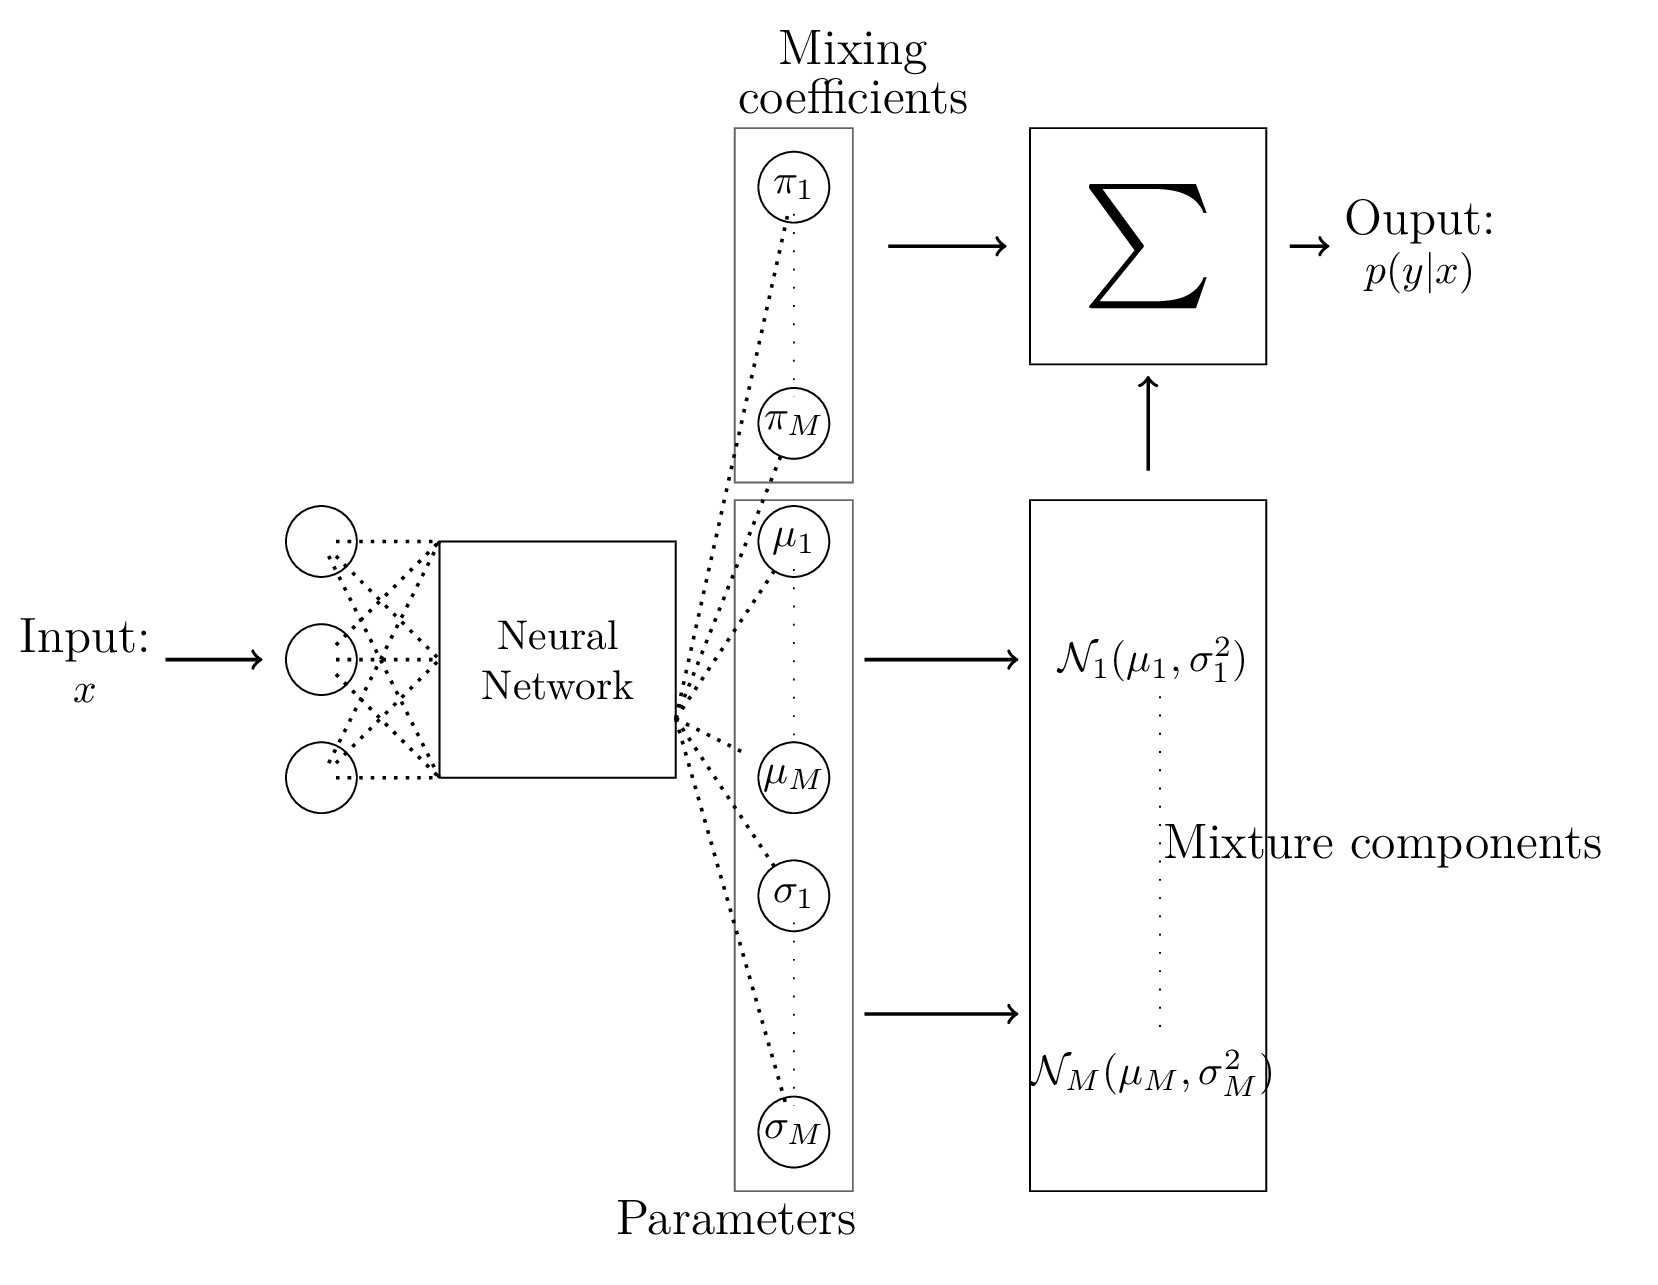
\includegraphics[height=0.8\textwidth, width=0.9\textwidth]{figures/mdn.png}
    \caption[Mixture Density Network Architecture]{Structure of a Mixture Density Network. The Input \(x\) first gets passed through a neural network. The outputs of that are treated as parameters for a mixture model. The mixture model is a weighted linear sum of different distributions -- normal distributions in our case. To note is that the mixing coefficients (the weights for the sum) are also generated from the network.}\label{fig:mdn}
  \end{figure}
\end{center}

With MDNs we again use the nice property of neural networks as universal function estimators. Before we proceed further, however, we must place some restrictions on the outputs of the network. Let \(z_m^{\alpha}\), \(z_m^{\mu}\) and \(z_m^{\sigma}\) be the outputs of some neural network \(f(x;\omega)\) with some parameter set \(\omega\) where \(z_m^{\alpha}\) affect the mixing coefficients \(\alpha_m\) and \(z_m^{\mu}\) and \(z_m^{\sigma}\) affect the means and variances of the mixture components respectively.

Now we give the exact relationships between the outputs and the mixture's parameters. The mixing coefficients of the mixture obviously must sum up to one as they are to be treated as probabilities:
\begin{equation}
  \sum_{m=1}^M\alpha_m(x)=1
\end{equation}
We can achieve that by placing a \emph{softmax} function on the respective outputs \(z_m^{\alpha} \) of the network 
\begin{equation}
  \alpha_m = \frac{e^{z_m^{\alpha}}}{\sum_{j=1}^M e^{z_j^{\alpha}}}
\end{equation}
where \(z_i^{\alpha}\) are the outputs of the networks ``responsible'' for the mixing coefficients \(\alpha_i\). Transforming the outputs of a network into a probabilities in this manner was introduced in~\cite{bridle1990}.

The variances of the Gaussian distributions represent \emph{scales} and for that they must be positive. We ensure this through the use of an exponential function
\begin{equation}
  \sigma_m = e^{z_m^{\sigma}}
\end{equation}
This also avoids the problem when some of the variances goes to zero. The means \(\mu_m(x)\) are to be seen as \emph{location} parameters and in order not to introduce bias in the system we model them directly with the network's corresponding outputs
\begin{equation}
  \mu_m = z_m^{\mu} 
\end{equation}
With those definitions we can summarize -- for a network with \(M\) mixtures the output would be \(\{\mu_m, \sigma_m^2, \pi_m \}, m\in\{1,\ldots ,M\}\). With the outputs we can define a conditional probability distribution for the data
\begin{equation}
  p(Y|X) = \sum_{m=1}^M \pi_m(X)\mathcal{N}(y|\mu_m(X), \sigma_m^2(X))
\end{equation}
Now we just have to give a loss function to be minimized. Starting from probability perspective, we want to maximize the likelihood of the the observed data \(\{(x_n, y_n)\}_1^N\), This is given by a product over the likelihoods of each data point:
\begin{equation}
  \mathcal{L} = \prod_{n=1}^N p(x_n, y_n) = \prod_{n=1}^N p(x_n)p(y_n | x_n)
\end{equation}
The term \(p(x_n)\) does not depend on the networks weights and can be spared. As for the \(p(y_n | x_n)\) -- this is where the mixture model comes into play. The quantity to be maximized thus becomes
\begin{equation}
  \tilde{\mathcal{L}} =  \prod_{n=1}^N \sum_{m=1}^M \alpha_m(x_n)\mathcal{N}(y_n; \mu_m(x_n), \sigma_m^2(x_n))
\end{equation}
Maximizing \(\tilde{\mathcal{L}}\) is equivalent to minimizing
\begin{equation}
  \label{eq:log-like-sum-1}
  E = \sum_{n=1}^NE^n
\end{equation}
where \(E^n\) is the contribution of the \(n^{th}\) data point and
\begin{equation}
  \label{eq:log-like-sum-2}
  E^n = -\log(\sum_{m=1}^M \alpha_m(x_n)\mathcal{N}(y_n; \mu_m(x_n), \sigma_m^2(x_n)))
\end{equation}
This function \(E\) can be minimized with standard backpropagation technique (\cite{bertels2001}) as its derivatives are fully tractable. Exact expressions for the derivatives of \(E\) are derived and given in \cite{bishop1994} but we don't consider them here. Details on the implementation of the MDNs are given in \refsec{sec:impl-model}
\clearpage
\section{Model evaluation methods}\label{sec:criticism}
\noindent\emph{In this section we give formal explanation to our approach in evaluating the models we build.}
\subsection{Probabilistic Forecast}\label{sec:prob-forecast}
\emph{We first explain the difference between the considered stochastic regression models and classical ones.}
\subsubsection{Prediction spaces}\label{sec:pred-space}
Classical regression models produce a point estimate \(y_i^e\) for each sample data point \(x_i\) with an actual realization \(y_i\). In this thesis, however, we are interested in regression models whose output is probabilistic forecast \(F\) that can be identified with the associated \emph{cumulative distribution function} (\emph{CDF}) as described in \refdef{def:prob-for}. This introduces the notion of prediction spaces proposed in~\cite{gneiting2013}. A prediction space is a probability space tailored to the study of distributional forecasts (\cite{gneiting2014}). Formally speaking we have to consider the realized observation also as a distribution even thou in practice this is a single value. In the most general case, the elements of the prediction space can be seen as tuples \((F, Y)\) where \(F\) is the probabilistic forecast and \(Y\) is the true distribution. \(F\) is a CDF-valued quantity which caries some information about the training data, the models' parameters, certain assumptions that are considered met and other model specific properties. Let \(\mathcal{A}\) denote all of the possible information that is available to make a forecast and let \(\mathcal{L}\) be some conditional distribution. We can say that the forecast \(F\) is ideal relative to the information encoded by \(\mathcal{A}\) if \(F=\mathcal{L}(Y | A)\). This means that the forecast utilizes the information completely. 

In our concrete case, the model -- BNN or MDN -- is the mechanism which generates the forecast. The models are trained on the training set and thus can ``gather'' information about the data. When making a prediction about new data point, the models use the gathered data and produce a probabilistic forecast in form of either CDF or a set of samples drawn from the predicted distribution.
\subsubsection{Dispersion and sharpness}\label{sec:disp-sharp}
\emph{Dispersion} and \emph{sharpness} are properties of predictive forecasts that describe the relationship between the observed value and the prediction. In order to formalize them, however, we need to introduce the notion of probability integral transform. For more information on probability integral transform see~\cite{diebold1998},~\cite{gneiting2007},~\cite{dawid84}.

Again, let \(F\) be the predicted distribution (see \refdef{def:prob-for}) for an observation \(Y\) in the sense of \refdef{def:prob-for}. The \emph{probability random transform} (\emph{PIT}) is the random variable \(Z_F=F(Y)\). Intuitively the PIT is the value of the predictive CDF.\@

With that we can formally define what dispersion and calibration are. In the following definitions \(F\) and \(G\) are two forecasts and their PITs are respectively \(Z_F\) and \(Z_G\). We say that
\begin{itemize}
\item[-] the forecast \(F\) is marginally calibrated, if \(\mathbb{F}(y) = \mathbb{P}(Y \leq y)\, \forall y\in\mathbb{R}\).
\item[-] the forecast \(F\) is probabilistically calibrated, if its PIT \(Z_F\) has standard uniform distribution.
\item[-] the forecast \(F\) is overdispersed, if \(var(Z_F) < \frac{1}{12}\) and underdispersed if \(var(Z_{\text{F}}) > \frac{1}{12} \).
\item[-] the forecast \(F\) is more dispersed, if \(var(Z_F) < var(Z_G)\).
\end{itemize}

As mentioned in \refsec{sec:prob-regression} calibration has to do with both the observation and the forecast. According to~\cite{gneiting2014}, if a forecast is ideal relative to some information set then it is both marginally and probabilistically calibrated.

As explained in~\cite{gneiting2014} the sharpness of a given forecast describes the concentration of the distribution without consideration of the actual observed value. When it comes to forecasts for a real-valued variable, sharpness can be assessed in terms of the associated prediction intervals. The mean widths of these intervals should be as short as possible. 

In next section we'll explain a certain class of scoring rules that can evaluate a predicted forecast against the observed value with respect to the dispersion and sharpness properties i.e.\ they assign ``better'' score to forecast with ``better'' dispersion and sharpness.
\subsection{Proper Scoring rules}\label{sec:proper-scoring-rules}
Proper scoring rules allow us to measure the predictive capability of a given probabilistic forecast. Those rules can consider the sharpness as well as the concentration of the distribution. The generated scores are measurement of differences between a desired and generated distributions and thus we strive to minimize those scores. Proper scoring rules are explained in details in~\cite{gneiting2007}.
% We'll briefly look at the essence of the proper scoring rules.
A scoring rule assigns a numerical score \(S(F, y)\) to each pair \((F, y)\) of probabilistic forecast \(F\) in a form of probability distribution and an observed value \(y \in \mathbb{R}\). In general, a scoring rule is some function \(S:\mathcal{F} \times \mathbb{R} \rightarrow \mathbb{R}\) where \(\mathcal{F}\) is some class of probability distributions. A scoring rules generally evaluates a predicted distribution against an realized observation. Let the desired distribution be \(G\in\mathcal{F}\). Then we write
\begin{equation}
  S(F,G) =\mathbb{E}_G[S(F,Y)]
\end{equation}
for the expected score between \(G\) and the forecast \(F\). 
The rule \(S: \mathcal{F} \times \mathbb{R} \rightarrow \mathbb{R}\) where \(\mathcal{F}\) is proper if the following property holds
\begin{equation}
  S(G,G) \leq S(F,G),\quad \forall G,F \in \mathcal{F}
\end{equation}
This means that a proper scoring rules yields a minimal score for the true distribution of the observation.
% when the forecast and the true distribution are the same.
We consider three proper scoring rules. The following sections discuss these.
\subsubsection{Logarithmic score (LS)}\label{sec:ls}
The most straight forward scoring rule is probably the \emph{logarithmic score}. This scoring rule is well established. One of its first propositions is made in~\cite{good1952}. For a given density function \(f^p(x)\) that belongs to a predicted forecast, the LS is given by
\begin{equation}
  LS(f^p,y) = -\log \, f^p(y)
\end{equation}
where \(y\) is the realized observation. The LS is lower (i.e.\ better), if according to the predicted forecast, the true observation is more probable. The LS would be at its lowest if the observation \(y\) is the maximum of the density \(f^p\). In this case, the actual observation will be the most probable value for the prediction according to the generated forecast. It is clear that sharper distributions will have lower LS given the observations falls into them. More concentrated distributions have higher values for their densities and thus are more certain for given observation.

The LS is the basis for a class of scoring rules called \emph{local scoring rules}. Those are discussed in detail in~\cite{ehm2012}.

A possible disadvantage of the LS is that it requires the density function of the forecast in order to be calculated. If the forecast is not given in density form, the probability density function must be approximated. For simple distributions this may not be a problem but for complicated ones, a considerable amount of samples from the distribution may be required. This can make the LS impractical for some probability models.
\subsubsection{Continuously ranked probability score (CRPS)}\label{sec:crps}
The mentioned disadvantage of the LS is addressed by the so called \emph{continuously ranked probability score} (\emph{CRPS}). The CRPS uses the predictive cumulative distribution function (CDF) of the forecast to give it score. CRPS is denied as
\begin{align}
  \label{eq:crps}
  CRPS(F,y)  &= \int_{-\infty}^{\infty}(F(x) - \mathbbm{1}\{y \leq x \})^2dx \\
             &= \mathbb{E}_F|Y - y| - \frac{1}{2}\mathbb{E}_F|Y - Y'|
\end{align}
where \(Y\) and \(Y'\) are are independent random variables with CDF \(F\) and finite first moment and \(\mathbbm{1}\{y \leq x \}\) is the probability for \(y\) to be less than or equal to \(x \). The second part of the equation is derived and described in~\cite{rafteryg2007} and~\cite{matheson1976}. In plain, words the definition says that the CRPS is a quadratic measure of the difference between the forecast's CDF and the empirical CDF of the observation. In contrast to the LS, the CRPS considers the distribution as a whole and doesn't focus on one specific point. CRPS is well studied and it finds application in a lot of cases (see~\cite{ranjan2011} for weighted variant and~\cite{grimit2007} for usage for circular variables). \reffig{fig:crps} gives visual intuition of the CRPS. From the figure one can clearly see that if the variance of the predicted distribution is big, the CDF will have values different form \(0\) and \(1\) in bigger interval and thus the CRPS will be higher. This shows how the CRPS encourages forecasts to be sharper with their distribution.
\vfill
\begin{center}
  \begin{figure}[H]
    \centering
    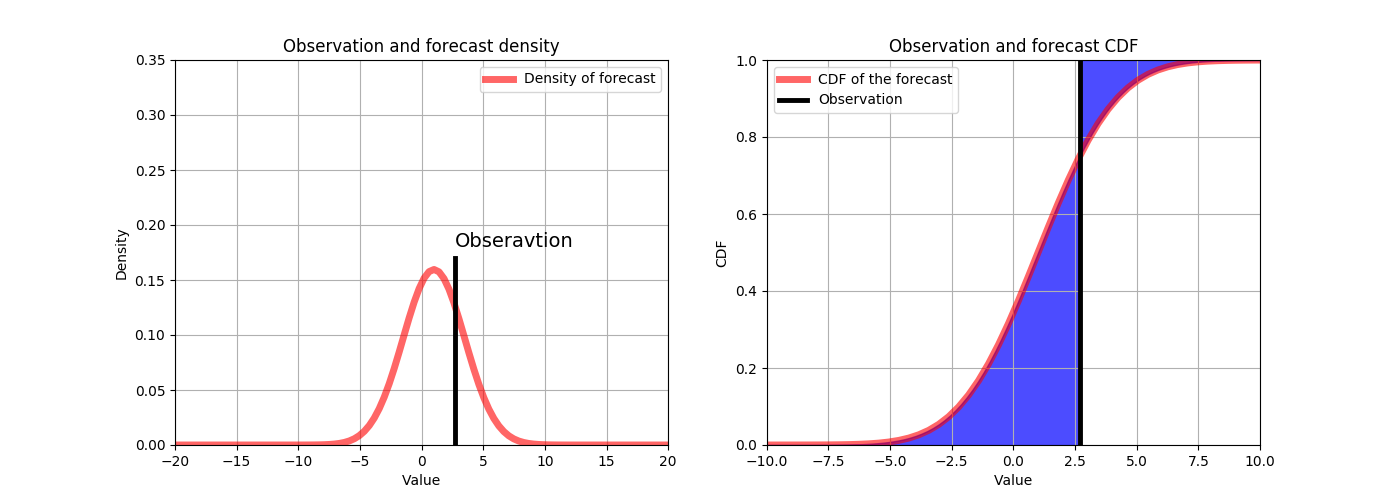
\includegraphics[height=0.41\textwidth, width=1\textwidth]{figures/crps.png}
    \caption[Continuous Rank Probability Score Intuition]{The square of the blue area is the value of the CRPS. Notice how if the predicted CDF were a step function (the case when the prediction is deterministic point estimate), the CRPS will be nothing more than the squared differnece between the observation and the prediction.}\label{fig:crps}
  \end{figure}
\end{center}
A useful property of the CRPS is that it reduces to the \emph{mean absolute error} (\emph{MAE}) if the forecast is deterministic. This allows us to compare probabilistic forecasts with point estimates in consistent manner (\cite{gneiting2014}).
\subsubsection{Dawid–Sebastiani score (DSS)}\label{sec:dss}
For complex distributions even the CRPS can be hard to evaluated as it requires some estimate of the integral in \refeq{eq:crps}. The \emph{Dawid–Sebastiani score} (\emph{DSS}), introduced in~\cite{dawid1999}, relies only on the first two central moments of a given predicted forecast \(F\). DSS is defined as
\begin{equation}
  DSS(F,y) =  \frac{(y-\mu_F)^2}{\sigma_F^2}+2\log(\sigma_F)
\end{equation}
Of the three rules the DSS is most simple to calculate as it requires only two simple metrics of the forecast. The only thing we need is the ability to draw samples from the distribution of the forecast and we can estimate the mean and variance.
\subsubsection{Computation of scoring rules}\label{sec:eval-rules}
In this thesis we deal with sets of data and we need to evaluate the scoring rules on certain number of data points -- on the test or train set. For this we take the average over the scores of all examples in a set. Let \(\{x_n, y_n\}_{n=1}^N\) be our set of interest and some model have generated set of forecasts \(\{F_n\}_{n=1}^N\) where forecast \(F_i\) is based on the features \(x_i\) and tries to predict the observation \(y_i\). The overall score \(\bar{S_N}\) of the scoring rule \(S\) then is
\begin{equation}
  S_N = \frac{1}{N}\sum_{i=1}^N S(F_i, y_i) \,
\end{equation}
This is the final metric on which we compare several probability models.

When it comes to calculating the rules themselves on concrete observations, there are explicit forms for the three rules, if the predicted forecast is a normal distribution. Those are given in \reftab{tab:rules-table} and taken from~\cite{gneiting2014}.

\begin{center}
  \renewcommand{\arraystretch}{1.7}
  \begin{tabular}{|l|l|}
    \hline
    \setlength\extrarowheight{5cm}
    Scoring rule \(S\) & \(S(\mathcal{N}(\mu, \sigma^2), y)\)\\
    \specialrule{.15em}{.05em}{.05em} %\hline
    \setlength\extrarowheight{5cm}
    Logarithmic score & \(\frac{(y-\mu)^2}{2\sigma^2} + \log(\sigma) + \frac{1}{2}\log(2\pi)\)\\
    \hline
    \setlength\extrarowheight{5cm}
    Continuous ranked probability score & \(\sigma(\frac{y-\mu}{\sigma}(2\Phi(\frac{y-\mu}{\sigma}) -1)\)\\
                       & \(\quad\quad + 2\phi(\frac{y-\mu}{\sigma}) - \frac{1}{\pi})\)\\
    \hline
    Dawid–Sebastiani score & \(\frac{(y-\mu)^2}{\sigma^2}+2\log(\sigma)\)\\
    \hline
  \end{tabular}
  \captionof{table}{Closed forms of the scoring rules for normal distribution}\label{tab:rules-table}
\end{center}

All of the examined model in the thesis can generate samples from their predicted forecasts. The DSS can thus be trivially calculated just through the empirical mean and variance of the generated samples. The predicted density function of the MDN is a sum of density functions of the mixture components (see \refsec{sec:mdn}) so it can easily be evaluated with the LS. For the BNN we use density estimation methods described in \cite{silverman1986} and \cite{scott2015} to calculate the LS. Empirical CDFs are trivially computable with sample data. For sample set \(\{x_i\}_i=1^n\) the empirical CDF is
\begin{align}
  &\bar{F_n}(t)=\frac{1}{n}\sum_{i=1}^n1_{x_i\leq t} \\
  &\text{wehre} \\
  &1_{a\leq t} =
    \begin{cases}
      1 &,\text{if}\, a \leq t \\
      0 &,\text{if}\, a > t 
    \end{cases}
\end{align}
With this function we can also calculate the CRPS in straightforward manner following the definition in \refeq{eq:crps}.
% With that we've covered all cases in the evaluation of our models.
\subsection{Feature Importance}\label{sec:feature-importance}
In order to asses the relative importance of the features used by the build models we use a method called \emph{permutation importance}. It is first described in~\cite{breiman2001} and it was applied to random forests. The techniques is also successfully applied in assessing the feature importance of ensemble forecasting\footnote{Ensemble forecasting is a method used in numerical weather prediction. Instead of making a single forecast of the most likely weather, a set (or an ensemble) of forecasts is produced~\cite{ensemble}.} methods for forecasting (\cite{lerch2018}). We closely follow the approach of \cite{lerch2018} by randomly shuffling each feature in the test and training sets and then look at the mean value of a given scoring rule. For each feature we examine the difference in the mean value of the scoring rules between the permuted and regular datasets.

We give formal definition of the described above. We consider a set of data \(\{x_n, y_n\}_{n=1}^N\) with feature vectors \(x_n\in\mathbb{R}^M\) and realized values \(y_n\in\mathbb{R}\). We define a matrix \(X\) with the features of all examples as
\begin{align}
  X &= \begin{bmatrix}
    x_{1} \\
    x_{2} \\
    \vdots \\
    x_{N}
  \end{bmatrix}
\end{align}
In this notation, the \(i^{th}\) row of the matrix are all of the features of the \(i^{th}\) example and the \(i^{th}\) column of the matrix are all of the \(i^{th}\) features of all examples. We further define \(F|x\) as the conditional forecast distribution given a vector of features of a input data point. We assume that \(F|x\) is predicted by some model. In essence we evaluate the importance of the used feature only in the context of the considered model. In this sense we examine which of the features have higher information value for the predictions of the given model.

Now we give formal definition for the permutation of the features. Let \(X_s\) denote the \(s^{th}\) column of the input data \(X\). Then the permuted set \(X^{\text{perm}_{\text{j}}}\) for the \(j^{th}\) feature is given by

\begin{equation}
  X^{\text{perm}_{\text{j}}} = 
  \begin{cases}
    X_{s},        & \text{if}\  j \neq s \\
    \pi(X_{(s)}), & \text{if}\  j = s
  \end{cases}
\end{equation}
where \(p(x)\) is some random permutation of the elements of the vector \(x\). Now we can give definition for the quantity that we call feature importance.
\begin{equation}
  \textit{Importance}(j) = \frac{1}{N}\sum_{n=1}^N (SR(F|X^{perm_j,(n)}, y_n) - SR(F|X^{(n)}, y_n) )
\end{equation}
where X\(^{\text{(n)}}\) is the feature vector of the \(n^{th}\) datapoint (i.e.\ the \(n^{th}\) row of the matrix \(X\)) and SR is some scoring rule -- CRPS, DSS or LS in our case.
\subsection{Rank Histogram}\label{sec:rank-hist}
\emph{Rank histograms} (sometimes called \emph{verification rank histogram}) are a tool for evaluating ensemble forecasts. See~\cite{hamill2001} for details. In our work, however, we adapt them to evaluate forecasts in form of probability distributions. The underlying assumption is that the ensemble member forecasts are distributed so as that the observed value behaves as a member of the ensemble. Let \([y_1^p,\ldots , y_M^p]\) be a \emph{sorted} by value ensemble where each \(y_i^p\in\mathbb{R}\) is a predicted value for the true observation \(y^t\). The rank of \(y^t\) according to the ensemble is an integer \(k\) such that
\begin{equation}
  rank(y^t)=
  \begin{cases}
    0,   & \text{if}\  y^t < y_1^p \\
    k,   & \text{if}\  y_{k}^p \leq y^t < y_{k+1}^p  \\
    k+1, & \text{if}\  y_{k+1}^p <  y^t  \\
  \end{cases}
\end{equation}
In our case the sorted ensemble is just a sorted sequence of drawn samples from the distribution predicted by the given model. We calculated the rank of each observation and then create a histogram with certain number of bins. To be noted is that the number of bins is considerably less than the number of samples. The amount of samples drawn from each model for each observation is in the order of tens of thousand while the number of bins for the rank histogram is no more than twenty.

For a well calibrated forecast, the rank histogram should be uniform. \texttt{U}-shaped histograms indicate underdispersed predictive distributions, whereas hump or inverse-\texttt{U}-shaped histograms correspond to overdispersed predictive distributions. These considerations are described in~\cite{gneiting2014},~\cite{diebold1998} and~\cite{hamill2001}. If the histogram is uniform we can say that the observation behaves as a sample from the forecast. This is essentially the behavior which a good forecast should exhibit. \reffig{fig:rank-hist} illustrates the said about rank histograms.
\begin{center}
  \begin{figure}[H]
    \centering
    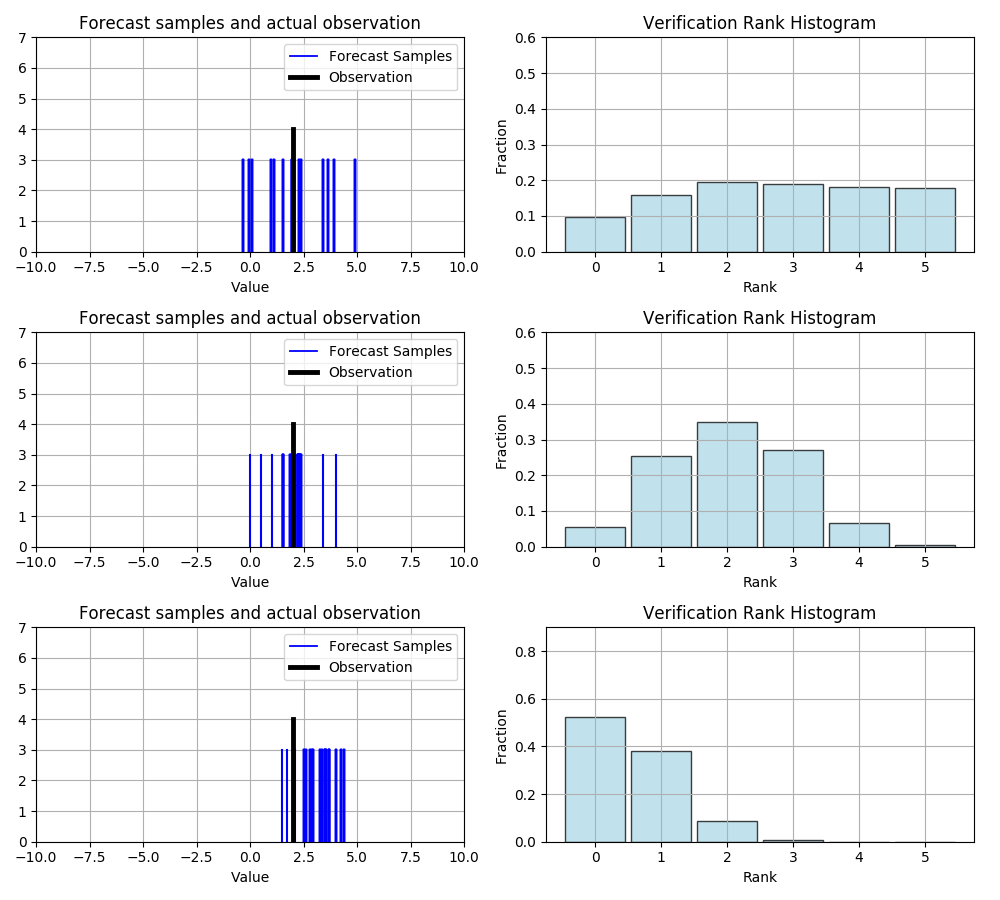
\includegraphics[height=0.75\textwidth, width=0.9\textwidth]{figures/verification_histogram.png}
    \caption[Rank Histogram Example]{Histograms illustrating different types of distributions with respect to the actual observations. To note is that on left we give only one example of samples drawn form the distribution in respect to a given observation. We assume that the sample sets for the other observations are similar and that this will produce the respective histograms on the right. A rank histogram cannot be given for a single observation and a single set of drawn samples.}\label{fig:rank-hist}
  \end{figure}
\end{center}
\subsection{Predictive performance check}\label{sec:pred-check}
\noindent\emph{In this section we explain how can we formally test if one forecasting model is better than another one.}

In order to conclude which one of given models is batter than the other ones, we want something more than just their average score of some rule over a test set. We introduce a statistical test -- the \emph{Diebold–Mariano test} -- which can asses the predictive performance of two forecasting methods in respect to one another and conclude which of them is better at predicting some data. The use of this particular test is suggested in~\cite{gneiting2014} and we follow and explain the approach given there.

Let \(F\) and \(G\) be two competing forecasting methods and let \(F_i \) and \(G_i \) be the forecasts each of the corresponding models produces for the actual observation \(y_i \). We can asses which of the methods has better predictive capabilities with the following approach. First we calculate the average values of some proper scoring rule over the entire test set with \(n\) observations
\begin{equation}
  \bar{S}^F_n=\frac{1}{n}\sum_{i=1}^nS(F_i, y_i) \quad \text{and} \quad \bar{S}^G_n=\frac{1}{n}\sum_{i=1}^nS(G_i, y_i)
\end{equation}
where \(S \) is some proper scoring rule. Then we calculate the metric
\begin{equation}
  t_n=\sqrt{n}\frac{\bar{S}_n^F-\bar{S}_n^G}{\hat{\sigma}_n}
\end{equation}
where
\begin{equation}
  \hat{\sigma}_n^2=\frac{1}{n}\sum_{i=1}^n(S(F_i,y_i)-S(G_i,y_i))^2
\end{equation}
This approach is known as the Diebold–Mariano test and it is first introduced in~\cite{diebold95}. The method is a statistical test of equal forecast performance. The null hypothesis is that the two forecasting methods predict the data equally bad or good. This means that we cannot prefer one of the methods over the other. If the null hypothesis is rejected, we can say which of the two is better than the other. Under the null hypothesis, the quantity \(t_n\) follows the standard normal distribution -- \(\mathcal{N}(0,1)\). This makes it particularly easy to calculate the corresponding \(p\)-value of the test. Given the \(p\)-value is small enough, the method \(F\) is preferred if \(t_n\) is negative, whereas \(G\) is preferred if \(t_n\) is positive (see~\cite{gneiting2014}).

\noindent Detailed information on the Diebold–Mariano test can be found in~\cite{diebold2015}.
\clearpage
\section{Results}\label{sec:res}
\emph{In this section we present the results from the evaluation of the trained models.}
\subsection{Methodology and data}\label{sec:preprop-meth}
\noindent
\emph{We first describe exactly what kind of datasets we use to train the model and what feature considerations we make.}

As described in \refsec{sec:data}, the data comes from different places and further more it is in different formats. Therefore we are responsible for generating the final datasets on which we train the models. This allows us to be flexible in the used data and therefore be able to investigate how the different resolution of the data affects the performance of the models. We describe the generation process in details in \refsec{sec:prep-data}. We have generated three different datasets:
\begin{itemize}
\item Daily averaged data -- For the whole considered period -- the year of 2017 -- we take the average pollution value (PM10 and PM2.5) of each sensor for each day. We treat the vector of those values as a single entry in the dataset. Naturally this means that we have \(365\) entries in this dataset.
\item Twelve hourly averaged data -- Analogous to the daily average but we take the average values over twelve hour periods over the entire year. \(730\) entries in the entire dataset.
\item Hourly averaged data -- We consider the average pollution value of each sensor over each hour in the year. The count of entries in this dataset is \(8760\).
\end{itemize}
We look at the performance of the models over each set in the respective sections. In \reffig{fig:sensor-plots} we show plots of the values coming from a single sensor. On the size of the value vectors for entries in each datasets -- after the data cleaning (described in \refsec{sec:prep-data}) we are left with sixteen sensors from \emph{luftdaten.info} and we also have three LUBW sensors. This adds up to nineteen sensors over all. For each of those we have PM10 and PM2.5 values. This means that for each day, twelve hours or one hour we have thirty eight values. We next describe how we choose subset of those to train models predicting a given another one of them.

As said, we want to investigate how different data affects the performance of the models. For that, we consider several types of orthogonal criteria.
\begin{itemize}
\item \emph{Predicted LUBW sensor} -- As mentioned, there are altogether three LUBW sensors\footnote{We use sensor and station interchangeably}. The names of those are \emph{SBC}, \emph{SNTR} and \emph{SAKP}. We want to see the predictive performance of the models based on which of these stations we are trying to predict. Plots of the data coming from these sensors can be seen in \reffig{fig:lubw-plots}.
\item \emph{Pollution value type} -- The air pollution values that all of the sensors measure are PM2.5 and PM10. See \refsec{sec:data} for more information on the meaning of these values. In our implementation and considerations we call those \emph{P1} and \emph{P2} respectively (see \refsec{sec:prep-data}). While preprocessing the data, we have found out that P1 and P2 are highly correlated. On average their correlation is about \(0.95\). This means that they effectively measure the same thing and will only make the feature space overly complicated, if both are considered as predictors\footnote{We use predictors and features interchangeably}. For this reason we either train on P1 or P2 values while predicting P1 or P2 respectively.
\item \emph{Using the rest of the LUBW senors as predictor} -- We want to see the difference in predictive performance of the models based on including the rest of the LUBW stations as predictors. That it, how much better or worse become the models, if we use values of the two other LUBW stations when we predict the values of the third one.
\end{itemize}

The final distinction about the models that we make is based on hyper-parameters of each of them. For the MDNs we can choose mixture components count and the definitions of the hidden layers. For the BNNs those hyper-parameters are again the definitions of the hidden layers as well as the drawn samples from the model while calculation the stochastic gradient descent. We consider two MDN-models -- one with one hidden layer with \(512\) neurons and three mixture components and one with one hidden layer but with \(1024\) neurons in it and again three mixture components. Both of the models were trained for maximum of six million and three thousand iterations so we give those models the names \texttt{mdn\_l[512]\_i6300000\_mc3}\footnote{The \texttt{l} signifies the layers, the \texttt{i} the iterations and \texttt{mc} the mixture components} and \texttt{mdn\_l[1024]\_i6300000\_mc3} respectively. When it comes to the BNNs, we only trained one model with one hidden layer and \(512\) neurons in it, where the drawn samples for the gradient calculation were \(800\). The BNNs were trained for maximum of \(3200\) iterations. The id of the BNNs is therefore \texttt{bnn\_l[512]\_i3200\_s800}.

Each of these distinctions in the construction of the models can be made independently of the other ones. We consider all possible combinations and we compare the results in \refsec{sec:eval-model}. By the training of the models, we used 75\% of the available data for the and the rest was used for the evaluation. All of the considered results are over the test set. To note is that the test-train split is not random. With the built models we want to predict future values of the sensors. Therefore we always split the data while preserving the order of the values -- from the start of the year till the end. In this sense, we always take the ``first'' 75\% of the values in the corresponding dataset and we use them as train-set and we try to predict the values from the ``future'' of the year.

We like to note that the training of the BNN models took significantly longer that than the training of the MDNs. All of the models were trained on a cluster of computers and overall one hundred and forty CPUs were used. The training of all of the MDNs took no longer than four days while the average paste of the BNNs was one trained model per day. 
\begin{figure}[H]
  \centering
  \begin{subfigure}[t]{0.32\textwidth}
    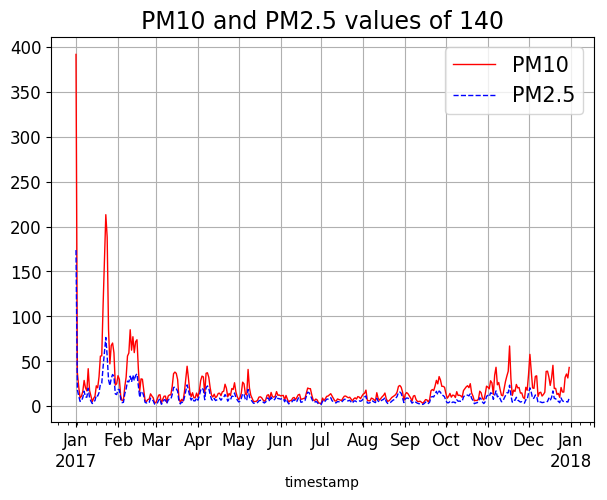
\includegraphics[width=\textwidth,height=6cm]{figures/plots_1d/140_plot}%
    \caption{Senor-ID: 140, daily average}
  \end{subfigure}
  %%%%%%%%%%%%%%%%%%%%%%%%%%%%%%%%%%%%%%%%%%%%%%%%%%% 
  \begin{subfigure}[t]{0.32\textwidth}
    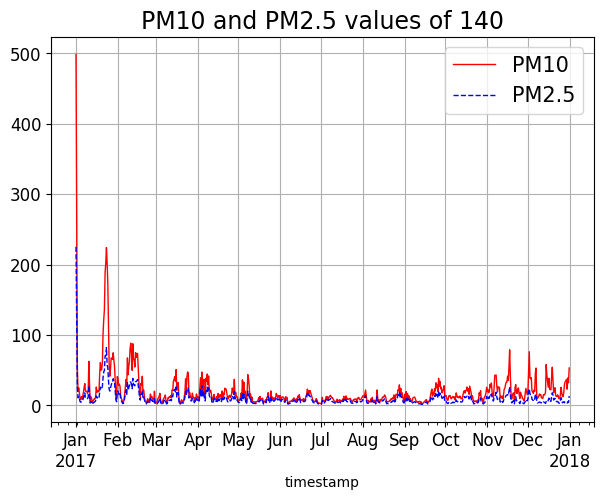
\includegraphics[width=\textwidth,height=6cm]{figures/plots_12h/140_plot}%
    \caption{Senor-ID: 140, twelve hour average}
  \end{subfigure}
  %%%%%%%%%%%%%%%%%%%%%%%%%%%%%%%%%%%%%%%%%%%%%%%%%%% 
  \begin{subfigure}[t]{0.32\textwidth}
    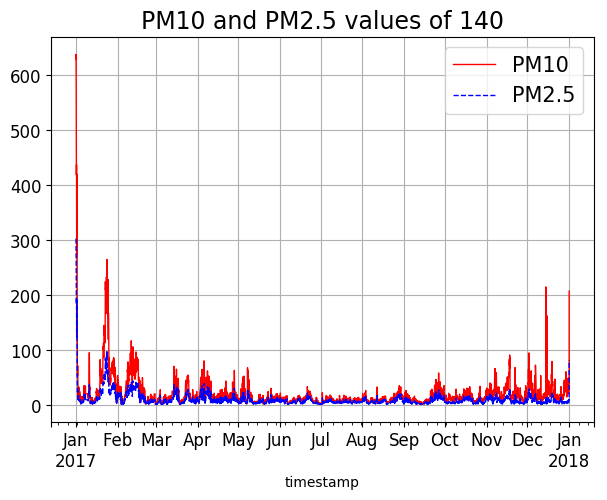
\includegraphics[width=\textwidth,height=6cm]{figures/plots_1h/140_plot}%
    \caption{Senor-ID: 140, hourly average}
  \end{subfigure}

  \begin{subfigure}[t]{0.32\textwidth}
    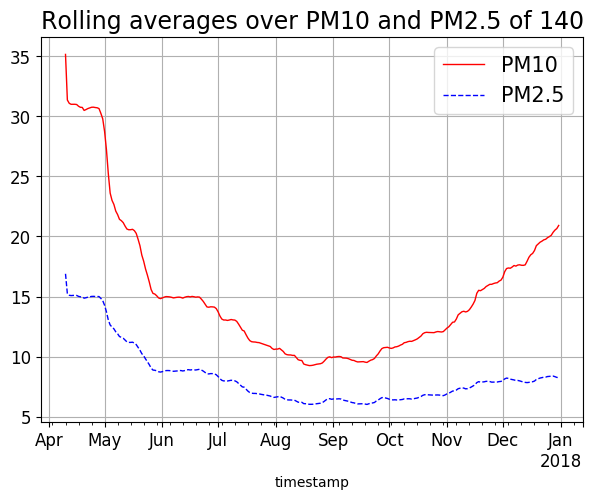
\includegraphics[width=\textwidth,height=6cm]{figures/plots_1d/140_rolling_plot_}%
    \caption{Senor-ID: 140, daily average, moving average}
  \end{subfigure}
  %%%%%%%%%%%%%%%%%%%%%%%%%%%%%%%%%%%%%%%%%%%%%%%%%%% 
  \begin{subfigure}[t]{0.32\textwidth}
    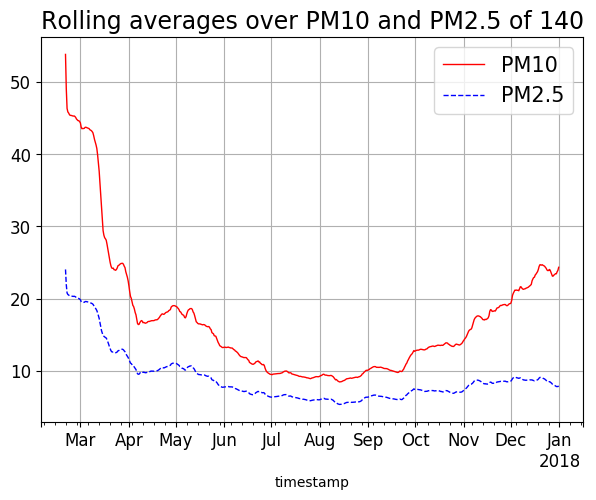
\includegraphics[width=\textwidth,height=6cm]{figures/plots_12h/140_rolling_plot_}%
    \caption{Senor-ID: 140, twelve hour average, moving average}
  \end{subfigure}
  %%%%%%%%%%%%%%%%%%%%%%%%%%%%%%%%%%%%%%%%%%%%%%%%%%% 
  \begin{subfigure}[t]{0.32\textwidth}
    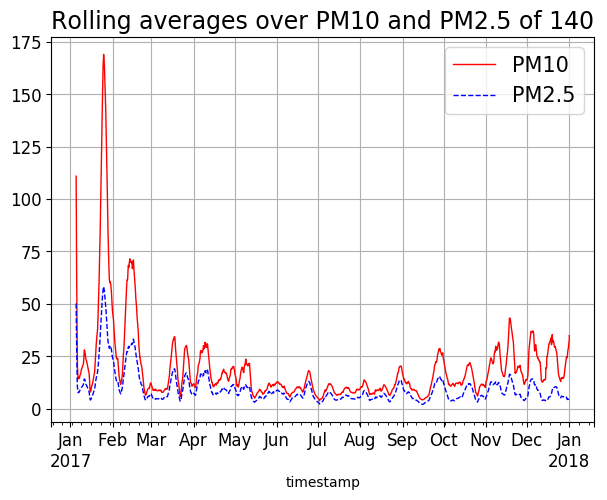
\includegraphics[width=\textwidth,height=6cm]{figures/plots_1h/140_rolling_plot_}%
    \subcaption{Senor-ID: 140, hourly average, moving average}
  \end{subfigure}      
  \caption[Sensor Data Plots]{Different views of the data from a single sensor. The P1 value is displayed in red and P2 in blue. The plots on the top row show the actual values over the entire year depending on the averaging period -- daily averaged in (a), twelve hour average in (b) and hour average in (c). (d), (e) and (f) show a moving average of 100 values of the respective plot above.}\label{fig:sensor-plots}
\end{figure}

\begin{figure}[H]
  \centering
  \begin{subfigure}[t]{0.32\textwidth}
    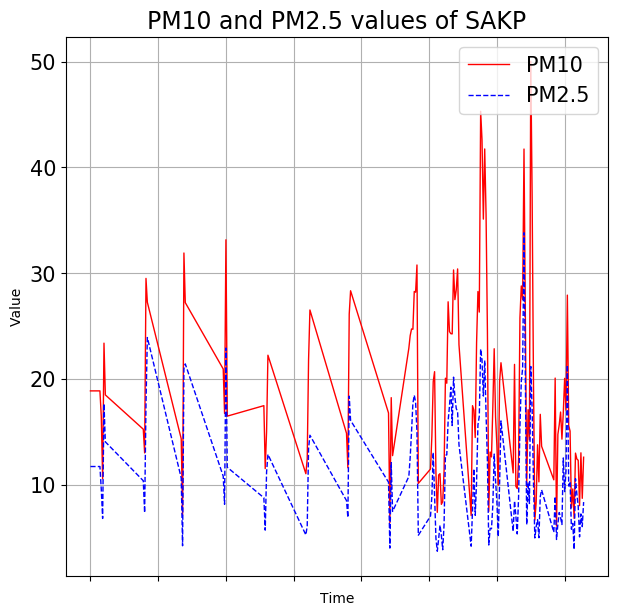
\includegraphics[width=\textwidth,height=6cm]{figures/plots_1d/SAKP_plot_P1_P2}%
    \caption{Sensor-ID: SAKP}
  \end{subfigure}
  %%%%%%%%%%%%%%%%%%%%%%%%%%%%%%%%%%%%%%%%%%%%%%%%%%% 
  \begin{subfigure}[t]{0.32\textwidth}
    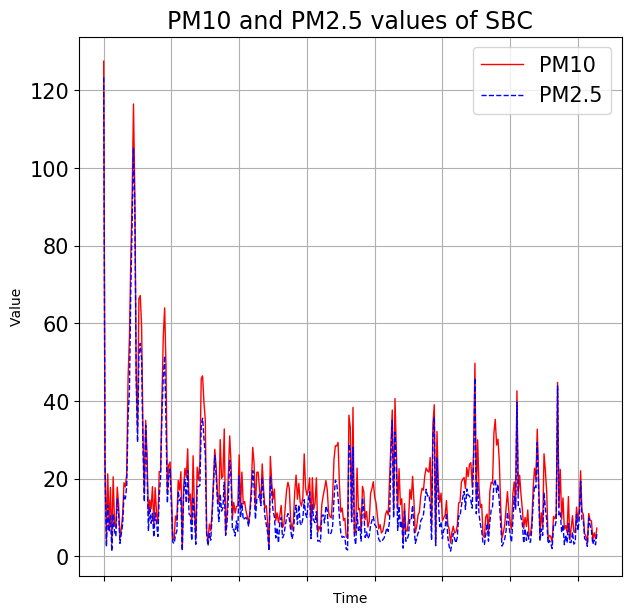
\includegraphics[width=\textwidth,height=6cm]{figures/plots_1d/SBC_plot_P1_P2}%
    \caption{Sensor-ID: SBC}
  \end{subfigure}
  %%%%%%%%%%%%%%%%%%%%%%%%%%%%%%%%%%%%%%%%%%%%%%%%%%% 
  \begin{subfigure}[t]{0.32\textwidth}
    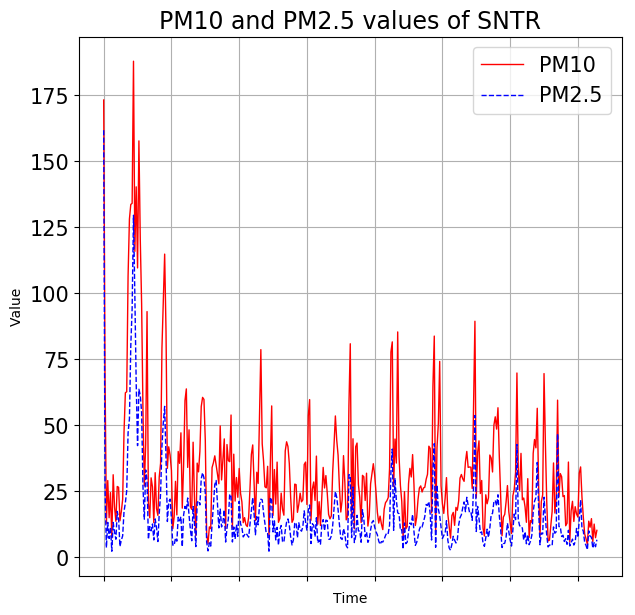
\includegraphics[width=\textwidth,height=6cm]{figures/plots_1d/SNTR_plot_P1_P2}%
    \caption{Sensor-ID: SNTR}
  \end{subfigure}

  \begin{subfigure}[t]{0.32\textwidth}
    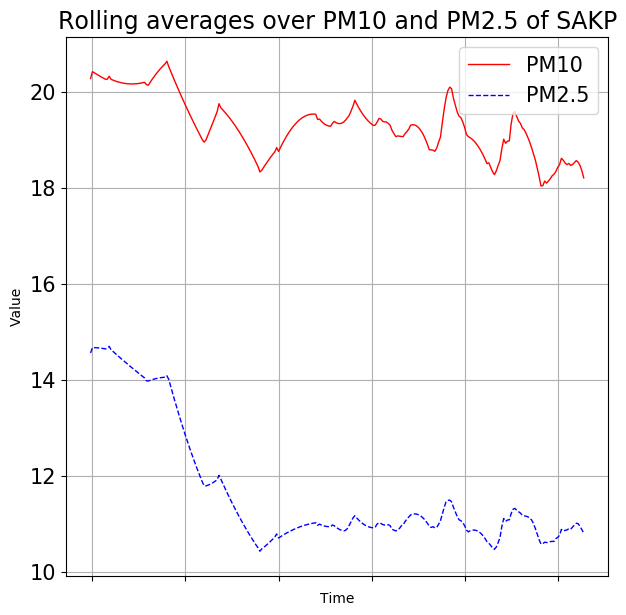
\includegraphics[width=\textwidth,height=6cm]{figures/plots_1d/SAKP_rolling_avg}%
    \caption{Sensor-ID: SAKP, moving average}
  \end{subfigure}
  %%%%%%%%%%%%%%%%%%%%%%%%%%%%%%%%%%%%%%%%%%%%%%%%%%% 
  \begin{subfigure}[t]{0.32\textwidth}
    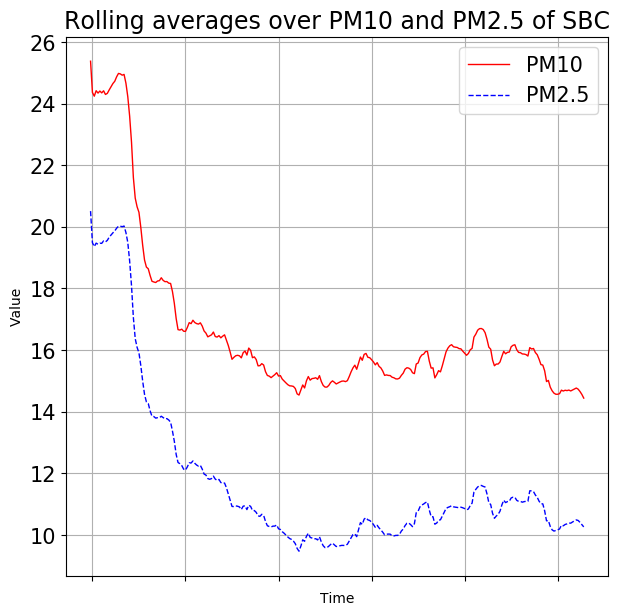
\includegraphics[width=\textwidth,height=6cm]{figures/plots_1d/SBC_rolling_avg}%
    \caption{Sensor-ID: SBC, moving average}
  \end{subfigure}
  %%%%%%%%%%%%%%%%%%%%%%%%%%%%%%%%%%%%%%%%%%%%%%%%%%% 
  \begin{subfigure}[t]{0.32\textwidth}
    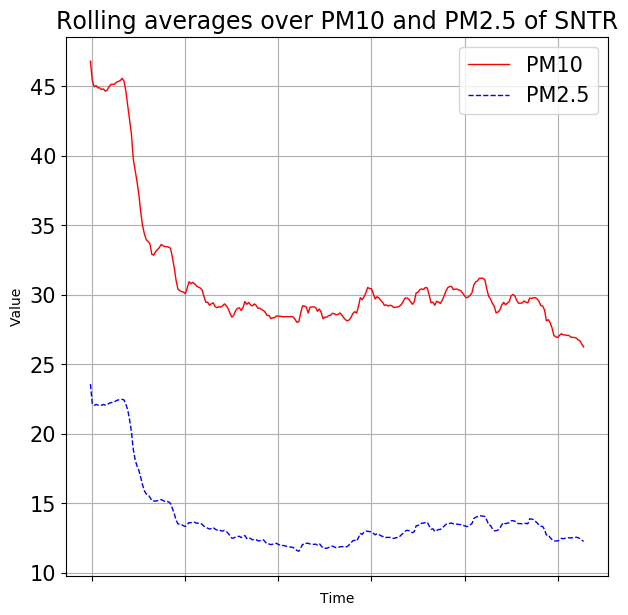
\includegraphics[width=\textwidth,height=6cm]{figures/plots_1d/SNTR_rolling_avg}%
    \subcaption{Sensor-ID: SNTR, moving average}
  \end{subfigure}      
  \caption[LUBW Data Plots]{The plots here show data from the tree LUBW sensors -- SAKP, SBC and SNTR respectively -- but only for the daily averaging period. The top row again shows the values for each day while the bottom is a moving average of 100 values. For explanation on the values of SAKP, see the note at the end of the chapter.}\label{fig:lubw-plots}
\end{figure}

When it comes to evaluation of the models, we evaluate each one differently generated model with the three proper scoring rules described in \refsec{sec:proper-scoring-rules}. We apply the feature importance technique from \refsec{sec:feature-importance} only with respect to the CRPS as in~\cite{lerch2018}. We look at the rank histograms of only some of the models. For details on rank histograms see \refsec{sec:rank-hist}. We also comment on the results of the predictive performance checks.

\emph{Note:} During the data preprocessing process we have found out that one of the LUBW sensors -- SAKP -- has data only for the last three months of the year. We have tried to interpolate the data for the rest of the year. This, however, means that the data from the sensors is almost unusable. We have decided to continue considering the sensor as we would, if this was not the fact. In the evaluation of the modes we hope to see results consistent with the made observation about the sensor. Namely:
\begin{itemize}
\item Predicting the values of SNTR is impossible as the values of the the sensor are generated independently of the values of the other sensors.
\item The importance of this sensors as predictor is very low for the same reason as above
\end{itemize}
We reference back this considerations while discussing the observed results.
\subsection{Evaluation of the models}\label{sec:eval-model}
As described in the previous section, we consider three different datasets based on the averaging period of the values. We look at the results on each of them in separate sections.
\subsubsection{One day period}\label{sec:res-1d}
\begin{center}
  \begin{figure}[htbp] \centering 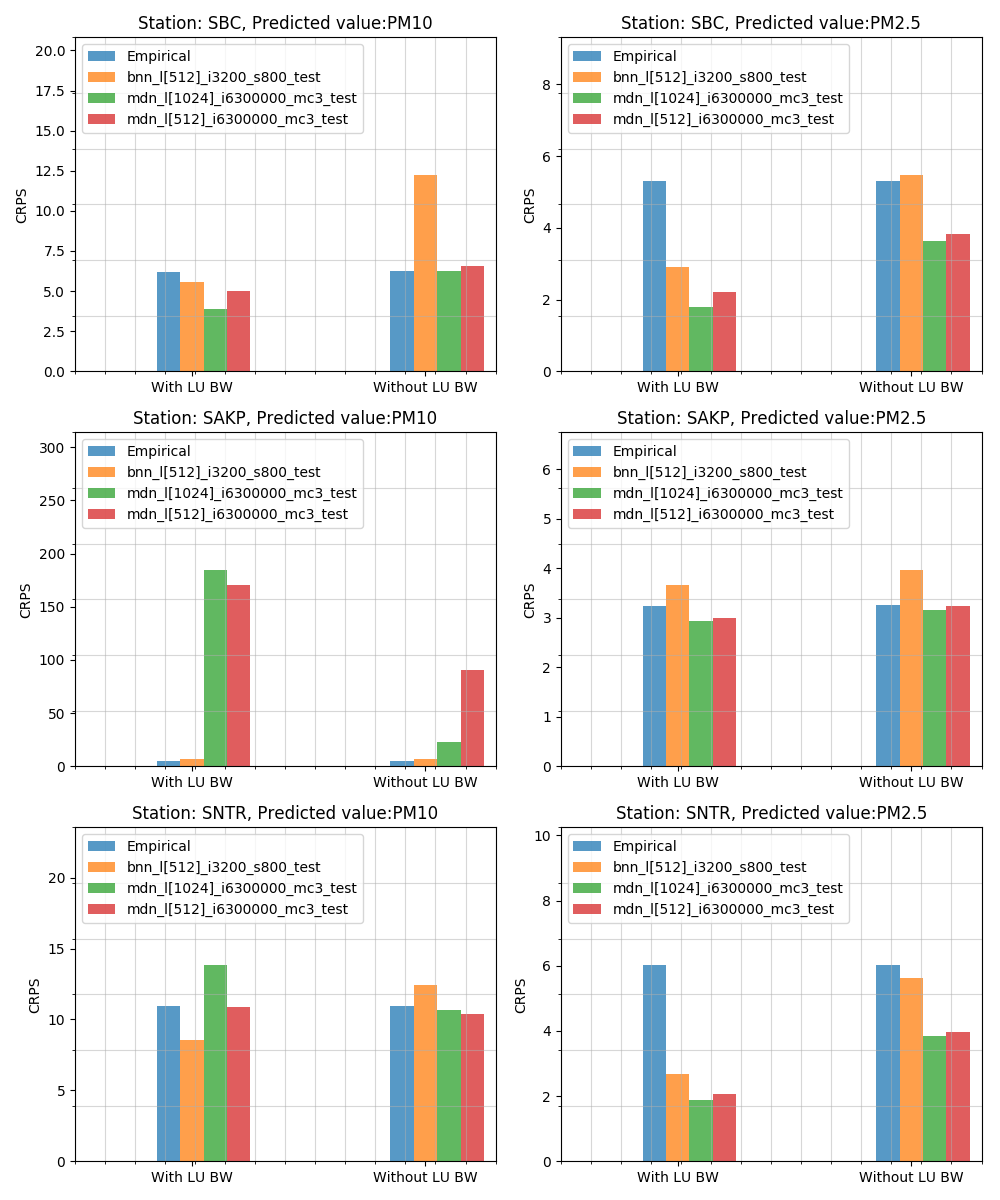
\includegraphics[height=1\textwidth,
    width=1\textwidth]{figures/figs_1d/results_plot_CRPS}
    \caption[CRPS results (daily average)]{CRPS values of the models
      (lower is better).}\label{fig:crps-1d}
  \end{figure}
\end{center}
\vspace{-1.3cm}

\reffig{fig:crps-1d} illustrates the results of the models with respect to the CRPS-rule. The plots in the first column show the results models predicting the PM10 value of the corresponding LUBW-sensor whereas those in the second column predict the PM2.5 value. The distinction between the predicted LUBW-sensors is made rowwise.

From the very first plot (predicting PM10 of station SBC) we see how the use of data from the LUBW-senors has effect on the performance of the models. Under the use of the LUBW-sensors the examined models outperform the set by the Empirical model baseline whereas this is not the case without it. This can also be observed while looking at the second plot (predicting PM2.5 of station SBC) where the performance of the BNN model drops significantly without the use of data from the LUBW-sensors. The change by the MNDs is, however, not that drastic and those models even manage to be better than the empirical model without the use of LUBW-data.

The results of predicting the values of SNTR are consistent with the first observations especially in the case of PM2.5. There we can also see the performance drop even though all of the models remain better than the Empirical one. We can again see that the sensibility to the use of LUBW-data is higher by the BNN model. It is interesting to note that in the case of the PM10 prediction, the performance of some of the MDNs is slightly higher without LUBW-data.

As it comes to predicting the values of SAKP, the results are quite inconsistent. This is to be expected as we explained in the previous section. All of the models cannot reliably predict the PM10 value. It is interesting to see that the scores are ``good'' for the prediction of the PM2.5 value. We assume, however, that because the models were unable to extract any meaningful relationship between the features and the predicted value, the variance of the predicted distributions had become large in order to compensate. By examining the plots of the made by the models predictions, we see that this is indeed the case. See \reffig{fig:mdn-bad}
\begin{center}
  \begin{figure}[H]
    \centering 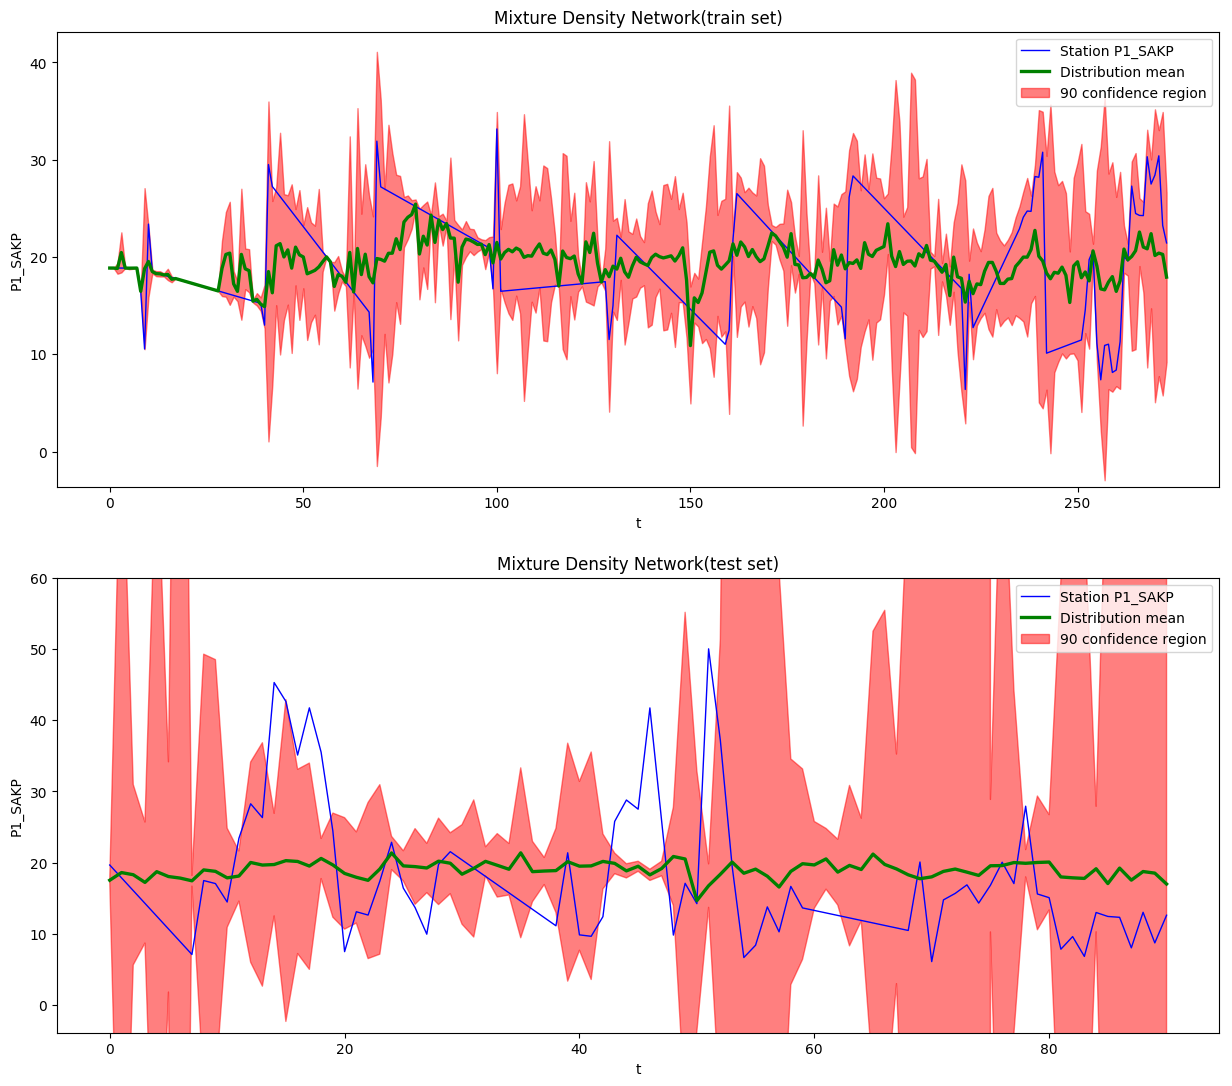
\includegraphics[height=0.55\textwidth,
    width=0.7\textwidth]{figures/mdn-bad}
    \caption[MDN plot on unreliable data ]{Plot of one of the MDN models where the predicted value is from SAKP. The plot on the top shows the results on the train set and the one on the bottom on the test set. We can clearly see that the variance of the predicted distributions is quite high most of the time. The plots of the other MDN models exhibit similar behavior.}\label{fig:mdn-bad}
  \end{figure}
\end{center}

Upon investigating the rank histograms of the models, we have found out that all of them are \texttt{U}-shaped. Rank histograms that are representative of all built models can be found in \refapp{app:g}. Rank histograms like these suggest that the models often fail to include the actual observation their confidence region. The observation falls then outside of the predicted distribution. This can be seen in the plots of the predictions of the models in \refapp{app:f}. The plots there even suggest that the models are prone to overfit the data and have significantly lower variance on the test set than on the train set. For compression, plots with the predictions of the empirical models are to be found in \refapp{app:h}

The results of the predictive performance checks are consistent with the observed CRPS values. Tables with results of the predictive performance checks are to be found in \refapp{app:e}. When predicting values of SBC or SNTR, both MDNs and the BNN reliably outperform the empirical model and the results supporting this are statistically significant with \(p\)-value lower than \(0.05\). According to the checks, the MDN with \(1024\) neurons in its hidden layer is the best model while predicting PM10 of SBC and BNN is the best while predicting PM10 of SNTR.

Plots with the rest of the scoring rules can be found in \refapp{app:c}

The results considered in this section can be found in tabular form with concrete numbers in \refapp{app:d}.
\subsubsection{Twelve hour period}\label{sec:res-12h}
\begin{center}
  \begin{figure}[H] \centering 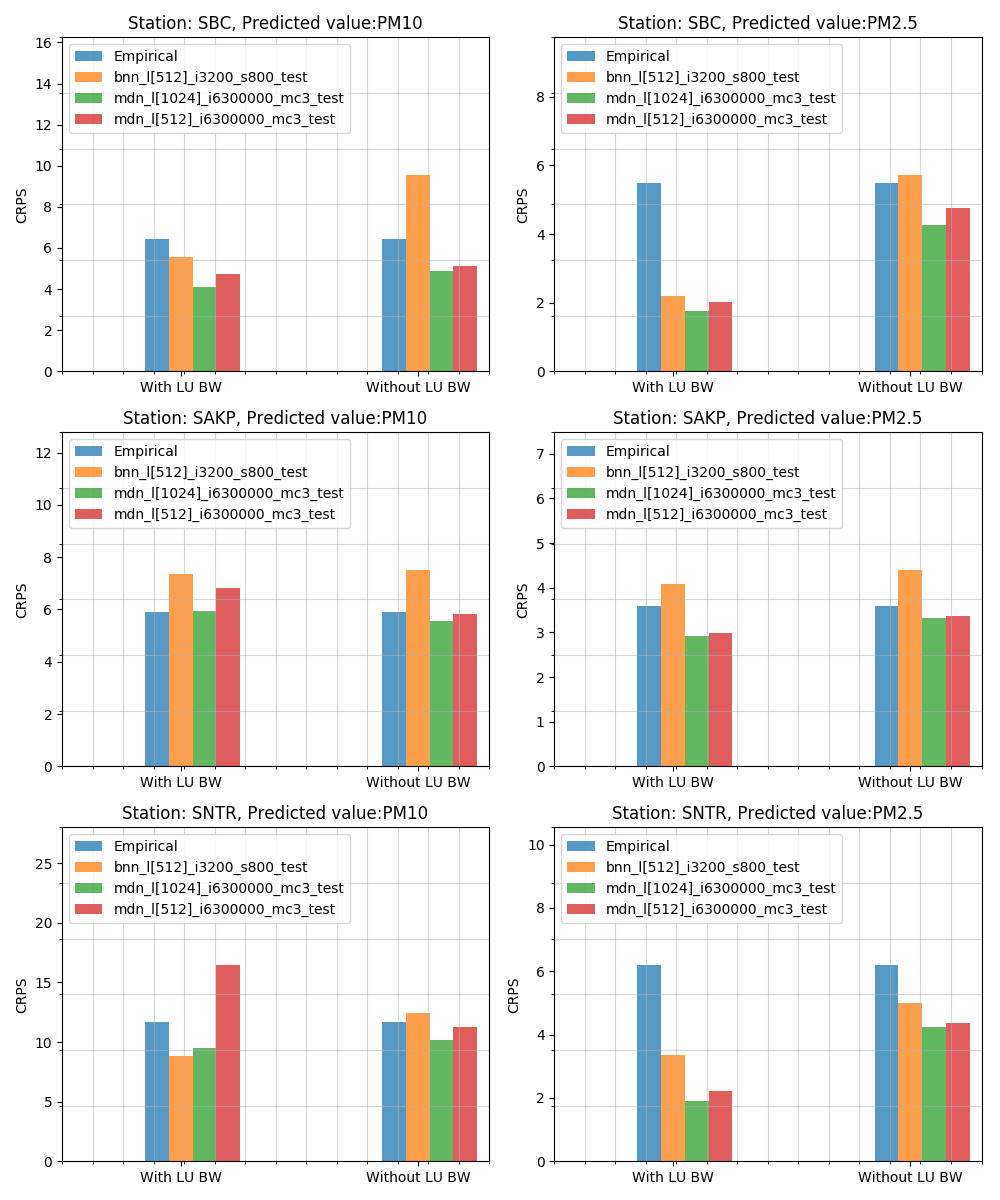
\includegraphics[height=0.9\textwidth,
    width=0.9\textwidth]{figures/figs_12h/results_plot_CRPS}
    \caption[CRPS results (twelve hourly average)]{CRPS values of the models
      (lower is better).}\label{fig:crps-12h}
  \end{figure}
\end{center}

\reffig{fig:crps-12h} is analogous to \reffig{fig:crps-1d} but the shown results are from models trained with twelve hourly averaged data. The observed in \reffig{fig:crps-12h} scores are consistent with the results from the previous section. In the prediction of the air pollution values of SBC we can again see how the BNN is sensitive to the use LUBW-data as features and the performance of the model drops without it in both cases - PM10 and PM2.5. What is interesting is that the both MDN models manage to remain better than the empirical model even without using values from LUBW-sensors. This suggest that the increasing the spatial resolution of the measurements from daily average to twelve hour average does not seem to have notable negative effect on the performance of the MDN models. We can even say that the performance is better as both of the models were worse than the empirical without using LUBW-data when they were trained with daily averaged data.

The tend is also noticeable in the prediction of SNTR values. There almost all of the models remain better than the empirical one regardless in all of the cases. To note is that one of the MDN models (the one given in red) has worse score than the empirical model in the case of predicting PM10 with the use of LUBW-data. We attribute that to poor starting training conditions of the model as its score is clearly not in the general trend of the results.

We again consider the scores for the models predicting SAKP values as unreliable. We see that in this case the scores of the models hardly change. This is consistent with the part of the results in the previous section.

Looking at the predictive performance checks (see \refapp{app:e}) of the models, we can see the same trend as suggested by the CRPS scores. The checks of the models trained with twelve hourly averaged data are statistically significant much more often than the ones trained with daily averaged data. This again leads us to believe that the increase of the time resolution of the averaged data has positive effect on the predictive performance of the models. The MDN with \(1024\) neurons in its hidden layer is the best model in the majority of the cases.

The rank histograms (see \refapp{app:g}) of the models continue to be \texttt{U}-shaped. We can, however, see that in the case of MDNs there is also noticeable concentration of values in the middle of the histogram. This means the models often succeed in generating a distribution encompassing the actual observed value.

The problem with overfitting the data is again suggested by the plot with the predictions of the BNN model in \refapp{app:f}. We can clearly see how the train data is predicted quite well but the one in the test set is merely approximated. At the start of the thesis we assumed that the considered types of models are robust to overfitting but the observed results suggest otherwise.
\subsubsection{One hour period}\label{sec:res-1h}
\begin{figure}[H] \centering 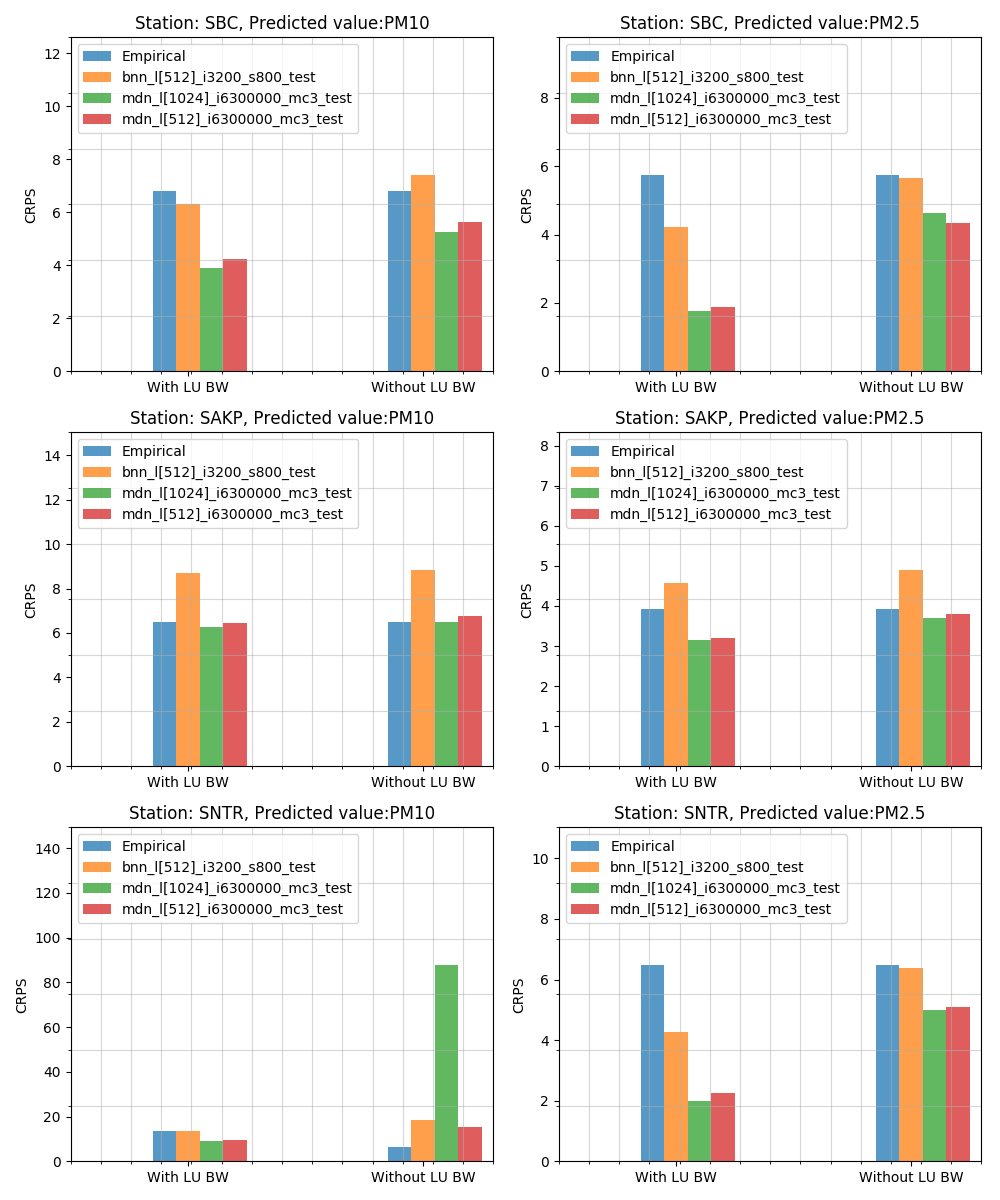
\includegraphics[height=0.9\textwidth,
  width=0.9\textwidth]{figures/figs_1h/results_plot_CRPS}
  \caption[CRPS results (hourly average)]{CRPS values of the models
    (lower is better).}\label{fig:crps-1h}
\end{figure}

\reffig{fig:crps-1h} presents the plots of the scores of the models trained with hourly averaged data. In it almost all of the cases are consistent with the results and trends from the previous sections.2

The scores of the models predicting SAKP again have little to no change and we consider them as unreliable. The sensitivity of the BNN models to the use of LUBW-data remains noticeable. We note however that the BNN models is better than the empirical in the case of predicting PM2.5 of SBC. This was not the case with the twelve hourly averaged data. This again suggests that increasing the time resolution does not make the models worse but rather it has positive effect on their CRPS scores relative to the empirical model.

In the case of predicting PM2.5 of SNTR, the scores of all of the models remain better than the empirical. This is, however, not true for the PM10 value. Even though the PM2.5 and PM10 values are highly correlated (see \refapp{app:a}) the models seems to have difference performance while predicting them. We assume this is due to the fact that PM10 varies in bigger intervals than PM2.5. This can be seen in the STD\footnote{Standard deviation}-plots in \refapp{app:b}.

The predictive performance checks for this averaging period are even more statistically significant than the ones for the twelve hour average. We can attribute this only to the use of data with higher time resolution. The MDN with \(1024\) neurons in its hidden layers is yet again the best model in almost all of the cases while looking at the statistically significant test metrics.

The general look of the rank histograms of the models for this averaging period is again less than ideal. The histograms again show that the models often fail to include the actual observation in the generated distribution. The rank histograms of the MDNs are, however, slightly better than the ones of the models from the previous sections.

As mentioned in \refsec{sec:res-1d}, plots with the rest of the scoring rules for each averaging period can be found in \refapp{app:c}. All of the considered scores can be found in tabular form with concrete numbers in \refapp{app:d}.
\subsection{Feature importance}\label{sec:model-feature-imp}
As seen in the previous section, only models trained a certain way achieve acceptable results. For this reason, we only looked at the feature importance results only of selected models. We again make the differentiation based on averaging period and we look at the results from each in three separate sections. We consider the feature importance data only with respect to the CRPS and for models that predict the PM2.5 values of SBC and SNTR.
\vfill
\subsubsection{One day period}
\begin{figure}[H]
  \centering
  \begin{subfigure}[t]{0.49\textwidth}
    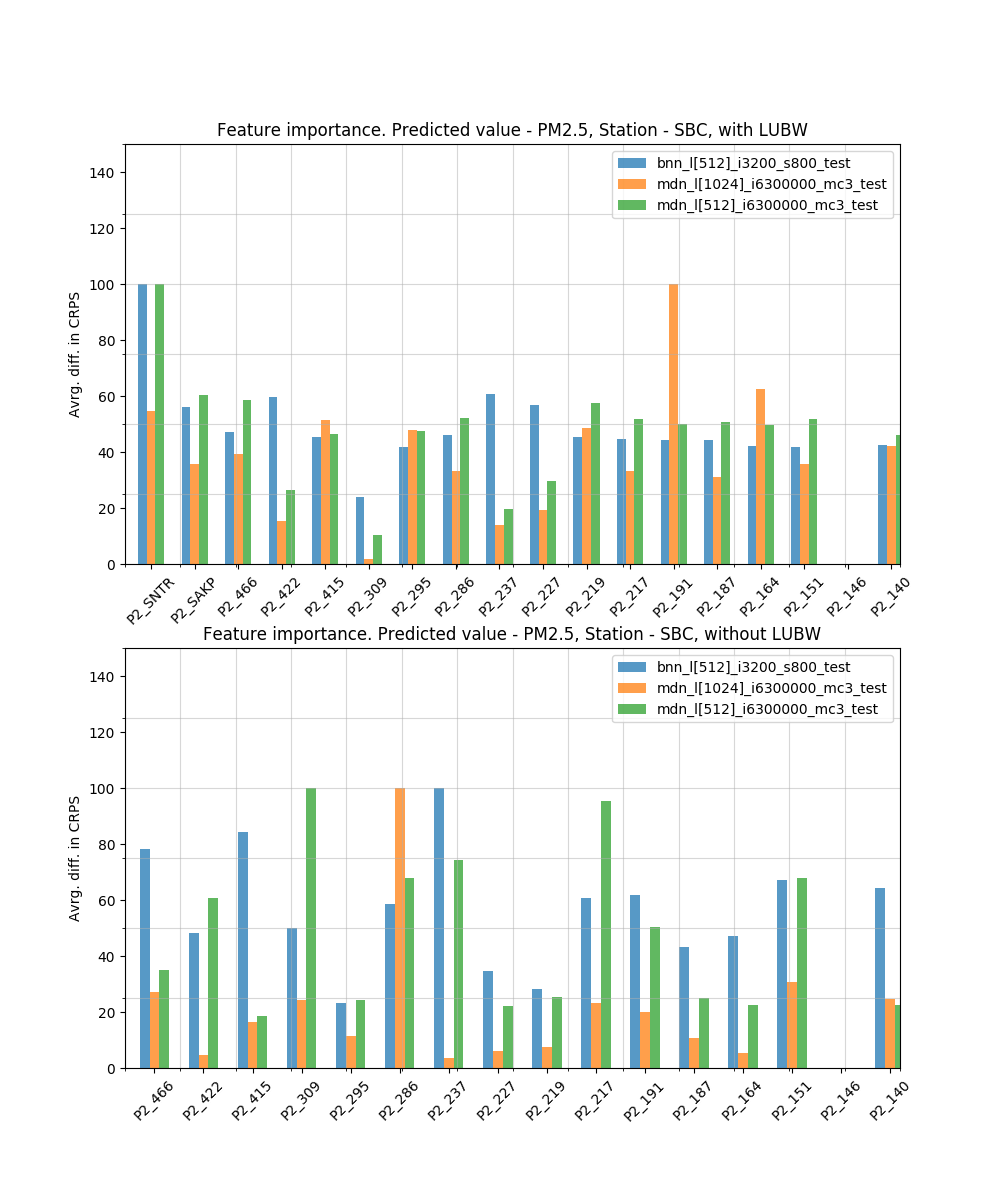
\includegraphics[width=\textwidth,height=1.2\textwidth]{figures/figs_1d/feature_importance_CRPS_SBC_P2}%
    \caption{Models predicting PM2.5 of the SBC LUBW-sensor.}
  \end{subfigure}
  %%%%%%%%%%%%%%%%%%%%%%%%%%%%%%%%%%%%%%%%%%%%%%%%%%% 
  \begin{subfigure}[t]{0.49\textwidth}
    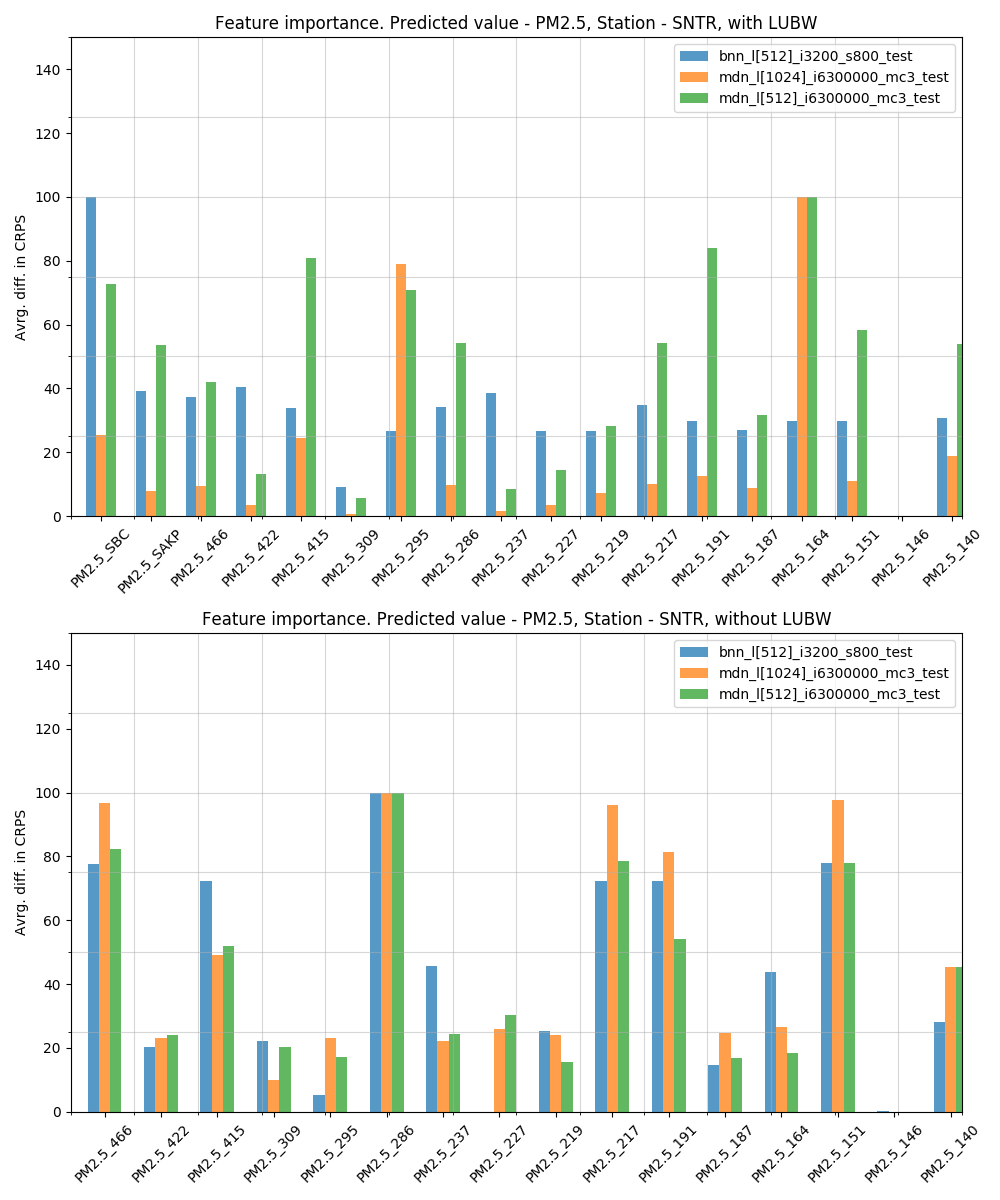
\includegraphics[width=\textwidth,height=1.2\textwidth]{figures/figs_1d/feature_importance_CRPS_SNTR_P2}%
    \caption{Models predicting PM2.5 of the SNTR LUBW-sensor.}
  \end{subfigure}
  \caption[Feature importance (daily average)]{The plots on the top show the feature importance results from models that use LUBW-data as features while those on the bottom are from models that do not.}\label{fig:feat-imp-1d}
\end{figure}
\reffig{fig:feat-imp-1d} illustrates the considered feature importance results. Looking at the plots we can make several notes about the importance of the different sensors.

A key observation to be made is that the sensor with ID \texttt{146} is consistently regarded as irrelevant. For each of the models and in every context this sensors seems to carry no information that can be used for the prediction of the given observations. Another sensors that has little importance in the models that use LUBW-data as feature is \texttt{309}.

If LUBW-data is used for the predictions, in both cases of predicting SBC and SNTR, the corresponding other LUBW-sensor\footnote{SNTR is case of predicting SBC and SBC in case of predicting SNTR} has maximum importance over the other sensors. This is to be expected as we consider the LUBW sensors as ground truth. It is interesting to note that the importance of the SAKP sensors is non-trivial and it is not much lower than the importance of the other sensors. We assume this is due to some random correlation between the interpolated data of SAKP and the predicted value. In this sense to think that this high importance of the SAKP sensor is accidental and does note represent reality.

If we focus on models not using LUBW-data we see how the sensor \texttt{286} stands out and has consistently high importance for two of the models. This appears to be true for both case of predicting SBC and SNTR. If the importance of this sensors is also high for the other two averaging period we would be able to conclude that it carries some relevant for the prediction information.

Another interesting point is how the BNN and one of the MDNs (the one shown in green) consistently have similar sensors with high or low importance. This can be seen as the green and the blue bars often go up and down together. This shows how two different models extract information from almost the same sensors in order to make their predictions. The MDN shown in orange exhibits slightly more irregular behavior but it also follows the general trend of which sensors are important and which are not. This is, however, not the case while predicting PM2.5 of SBC without the use of LUBW-data. There the MDN uses the sensor with id \texttt{286} almost exclusively. If we look at the performance of the MDN in \refsec{sec:res-1d}, we see that in the corresponding case, it is better than the empirical model. This means that this MDN can be better than the baseline even when the majority of the information for the predictions comes from a single non-LUBW sensor.
\subsubsection{Twelve hour period}
\begin{figure}[H]
  \centering
  \begin{subfigure}[t]{0.49\textwidth}
    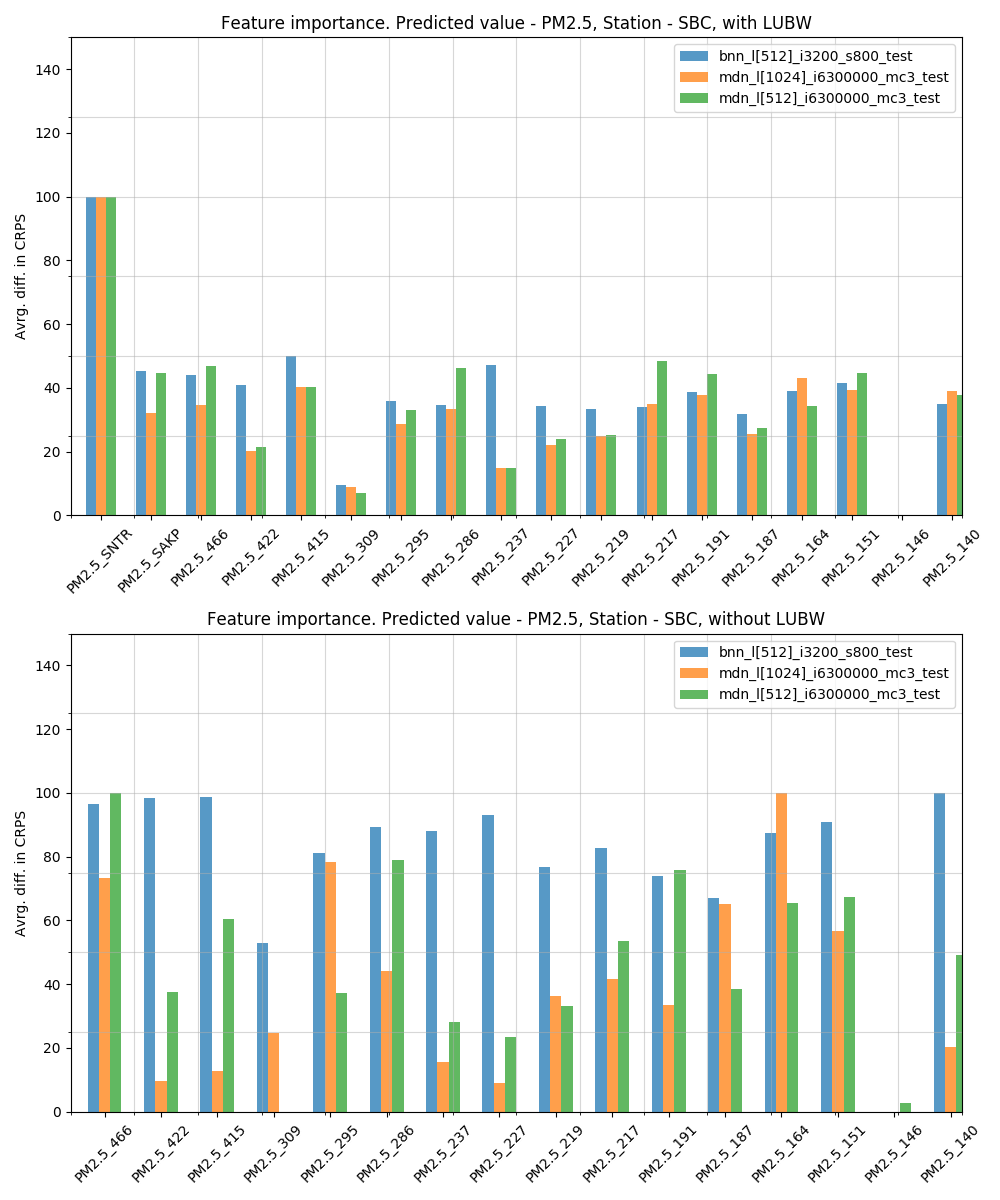
\includegraphics[width=\textwidth,height=1.2\textwidth]{figures/figs_12h/feature_importance_CRPS_SBC_P2}%
    \caption{Models predicting PM2.5 of the SBC LUBW-sensor.}
  \end{subfigure}
  %%%%%%%%%%%%%%%%%%%%%%%%%%%%%%%%%%%%%%%%%%%%%%%%%%%
  \begin{subfigure}[t]{0.49\textwidth}
    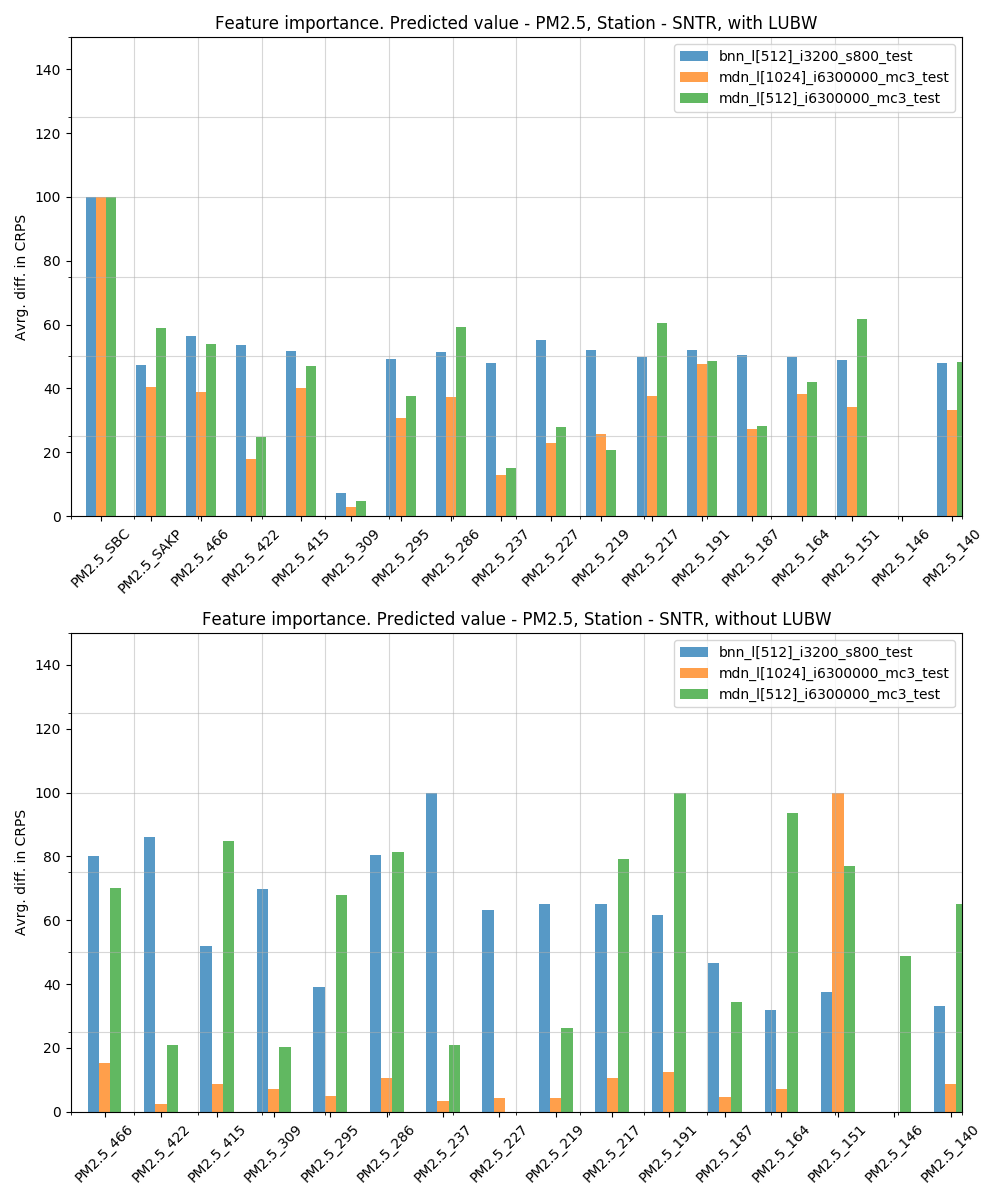
\includegraphics[width=\textwidth,height=1.2\textwidth]{figures/figs_12h/feature_importance_CRPS_SNTR_P2}%
    \caption{Models predicting PM2.5 of the SNTR LUBW-sensor.}
  \end{subfigure}
  \caption[Feature importance (twelve hourly average)]{The plots on the top show the feature importance results from models that use LUBW-data as features while those on the bottom are from models that do not.}\label{fig:feat-imp-12h}
\end{figure}
\reffig{fig:feat-imp-12h} presents plots with feature importance data from models trained with hourly averaged data. We can make almost the same observations s in the previous section but there are some differences.

We notice again how the \texttt{146} sensor has very little importance for almost all of the models except one in the case of predicting PM2.5 of SNTR without using LUBW-data as feature. The importance of the sensor with ID \texttt{309} also consistent with the results from the previous section.

If we look only at the feature importance plots of the models that use LUBW-data as feature, we see how the sensors tend to have similar importance for every model. This suggests that three different models extract similar connections between the predicted value and the predictors. In the previous section this was obvious only for two of the models. We assume that the increased time resolution of the averaged data allows the models to extract deeper relationships between the value to be predicted and the features.

We no focus on the models on the bottom plots. Here we again observe how the sensor \texttt{286} has high importance for two of the models -- the ones shown in blue and green. This was also the case in the previous section.

The MDN shown in orange has similar behavior where it almost uses a single sensor for its predictions. This time, however, this happens in the case of preciting PM2.5 of SNTR without the use LUBW-data. There we can see how the sensor with id \texttt{151} has very high importance while the other sensors have very low one. Based on this and on the observation from the previous section, we assume that this MDN model is prone to extract information from a single feature and use it for the predictions.
\subsubsection{One hour period}
\begin{figure}[H]
  \centering
  \begin{subfigure}[t]{0.49\textwidth}
    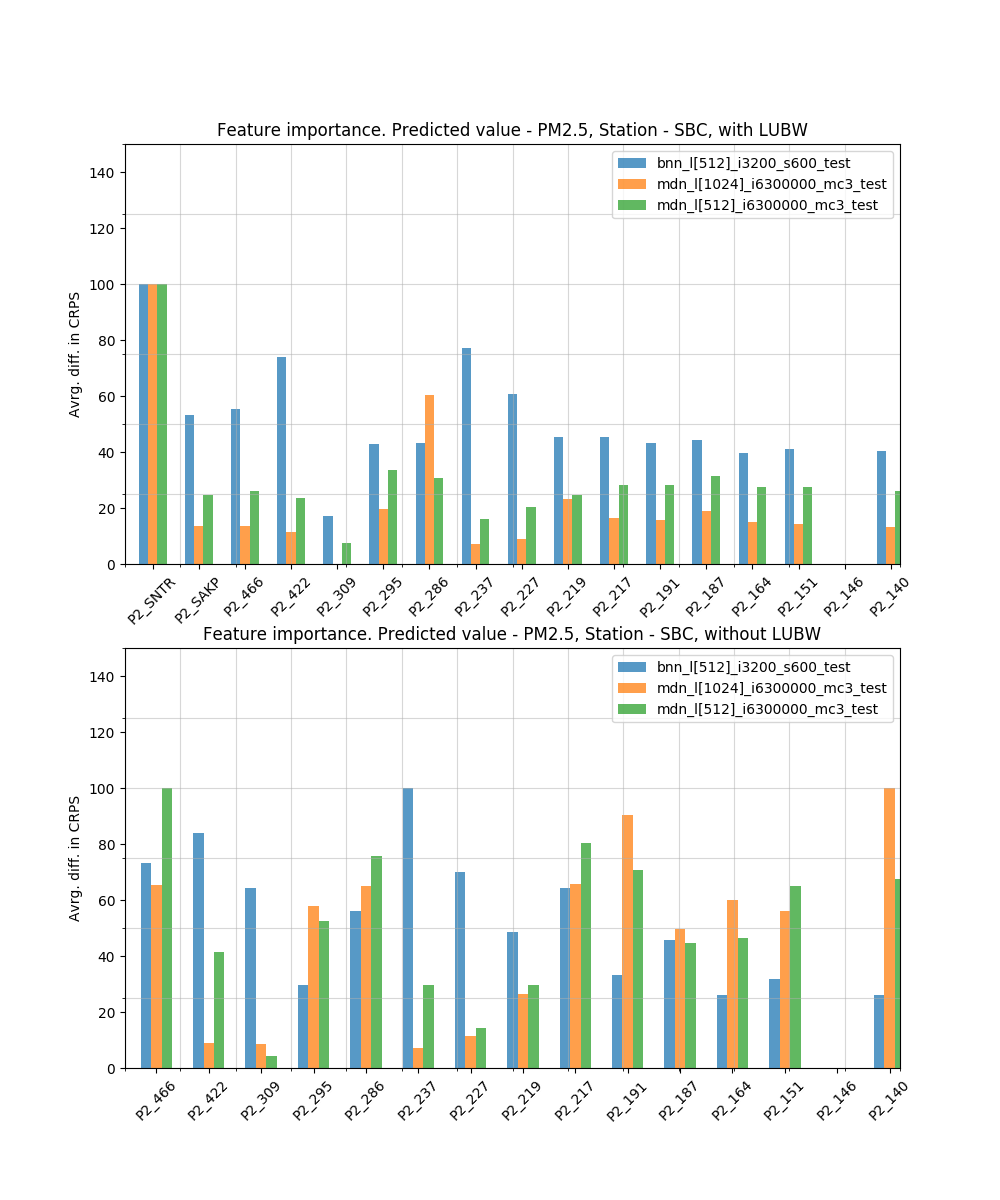
\includegraphics[width=\textwidth,height=1.2\textwidth]{figures/figs_1h/feature_importance_CRPS_SBC_P2}%
    \caption{Models predicting PM2.5 of the SBC LUBW-sensor.}
  \end{subfigure}
  %%%%%%%%%%%%%%%%%%%%%%%%%%%%%%%%%%%%%%%%%%%%%%%%%%% 
  \begin{subfigure}[t]{0.49\textwidth}
    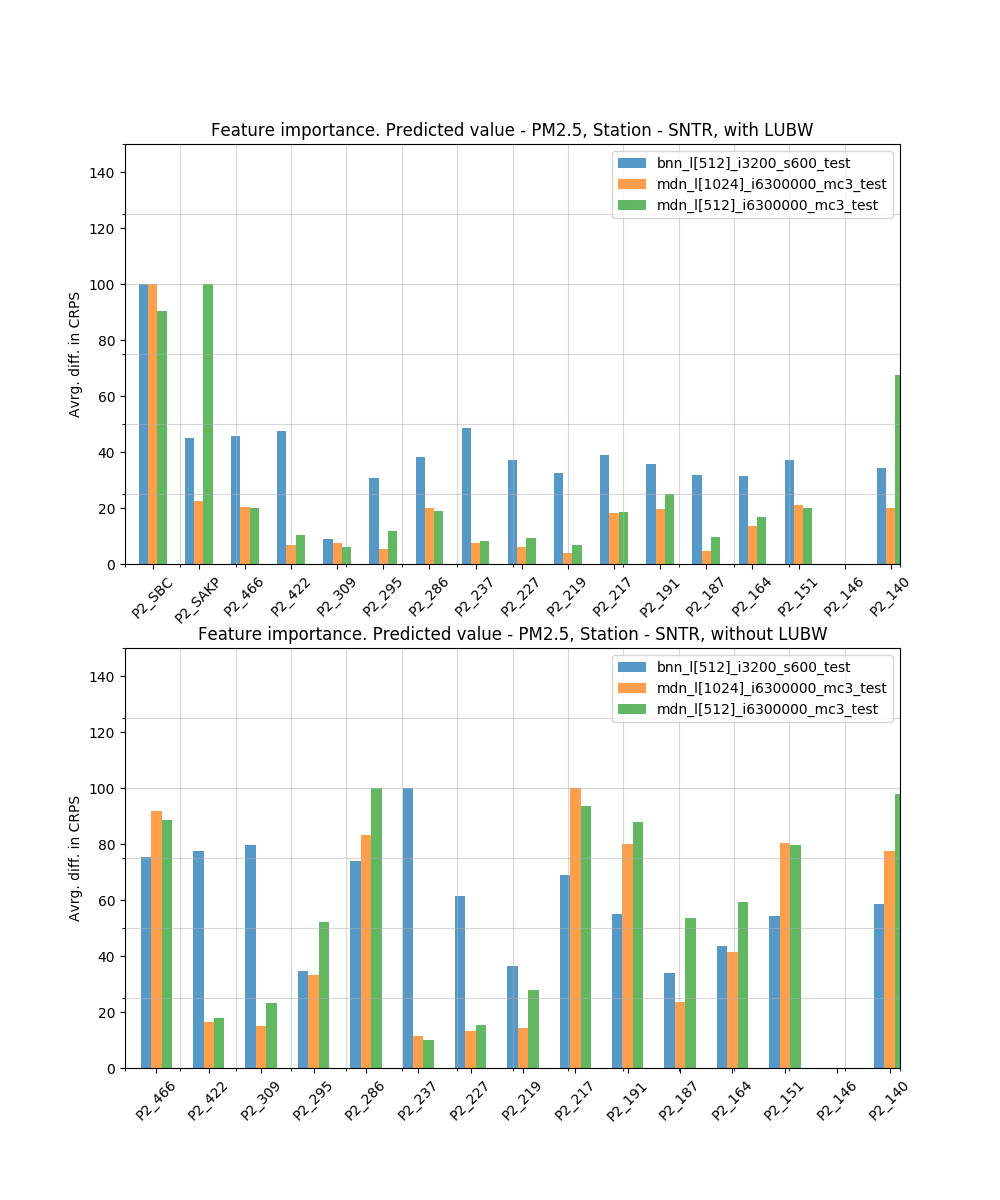
\includegraphics[width=\textwidth,height=1.2\textwidth]{figures/figs_1h/feature_importance_CRPS_SNTR_P2}%
    \caption{Models predicting PM2.5 of the SNTR LUBW-sensor.}
  \end{subfigure}
  \caption[Feature importance (hourly average)]{The plots on the top show the feature importance results from models that use LUBW-data as features while those on the bottom are from models that do not.}\label{fig:feat-imp-1h}
\end{figure}
Lastly we look at the feature importance results from the models trained on hourly averaged data. Plots of these results are given in \reffig{fig:feat-imp-1h}. The observations that we can made here are essentially the same as the one in the previous sections.

The SBC and SNTR sensors have again high importance. As seen in the previous results, the senor \texttt{146} caries no information for all of the models in all of the contexts and the sensor \texttt{309} has a relatively low importance when used together with LUBW-data as features.

A surprising result to see is that for the MDN shown in green SAKP has highest importance over all features. This is again probably due to a accentual correlation between the interpolated data of SAKP and the predicted value.

In the case of this  averaging period, the sensor \texttt{286} has high importance with respect to all of the models. In the previous sections this was true only with respect to the one of the MDNs and the BNN. With the averaging of maximal time resolution, however, it appears that every model can extract some meaningful information from this sensor.

We have clearly seen how across all averaging periods the feature importance results are consistent with one another. Based on this we can conclude that we have successfully identified couple of weak sensors in the network -- those with ides \texttt{146} and \texttt{309} -- as well as sensors that appear to have higher value than the others -- obviously SNTR and SBC but also probably \texttt{151} and \texttt{286} given the fact that one of the MDNs can produce reliable predictions almost purely based on one of the sensors. We have also followed the importance of the sensor with id \texttt{286} and seen that it consistently has high importance. 
\vfill
\clearpage
\section{Implementation}\label{sec:impl}
In order to enforce separation between the code and all of the data that the code acts upon, we place all of the generated data in the \texttt{env} directory of the project. This directory is added to the \texttt{.gitignore} file and the implantation in no way relies on its contents. The contents of the folder are fully generated by the implemented scripts. In the next sections we explain exactly what the generated content is and how it is generated.
\subsection{Used libraries}\label{sec:libs}
In order to make the data preprocessing, the implementation of the models and their evaluation easier, we use several standard machine learning libraries. For efficient array manipulation we use the popular \emph{python}\footnote{Programming language.} library \emph{numpy}, described in~\cite{numpy}. The higher level data processing is done through \emph{pandas}~\cite{pandas} and for the plotting of the results we employ the use of \emph{matplotlib}~\cite{matplotlib}. When it comes to the actual machine learning we use a lot of helper methods from \emph{scipy}~\cite{scipy} and \emph{scikit-learn}~\cite{scikit-learn}. The core library for the implementation of the models is \emph{Tensorflow}~\cite{tf}. For the easier handling of the implementation of MDNs and BNNs we use respectively two other libraries built on top of Tensorflow -- GPFlow~\cite{gpflow} and Edward~\cite{edward}. 
\subsection{Preparing the data}\label{sec:prep-data}
In \refsec{sec:data} we mentioned that the used public data is less than ideal. We have also outlined some of the problems that we found in the data. Now we explain how we deal with these problems. We have written several python scripts dealing with the preprocessing of the data. 

The raw data files are located under~\cite{luftdaten}. They are organized in folders by day. The folder for a given day contains different files from different sensor types. We are only interested in the air pollution data form the \emph{sds011} sensors. Each data file for this type of sensor is a text file with \emph{comma separated values} (\emph{CSV}) where each row has measurements for the PM2.5 and PM10 value (see \refsec{sec:data}), the location of the sensor, the time of day when the measurement was taken as well as the sensor-id. Our final goal in the data preprocessing in to generate a \emph{DataFrame}\footnote{A \emph{padnas}-object for easy data storage} where each column is labeled with sensor-id and either P1 (for PM2.5) or P2 (for PM10) and each row contains measurements of the corresponding values averaged over some periods of time. The periods of time in which we integrate\footnote{We use integrate and average interchangeably.} must be synchronized between all sensors. At the end we generate three different DataFrames from the data -- with averaging over whole days, over twelve hour periods and over one hour periods.

We try to automate everything from downloading the data, extracting the relevant pieces of it, sanitizing it and finally generating a single DataFrame object. As the data preprocessing is not the focus of this thesis, we do not explain each script in absolute detail but rather what happens in it.

All of the scripts we explain in this section require a configuration file. This file is \texttt{config.json}. In it we define certain properties for the scripts so that we can easily change them if necessary. In each of the data preprocessing scripts there is a \texttt{\_read\_config} method that loads the relevant for the script properties from the configuration file. In the next paragraphs we use property and field interchangeably. We also sometimes obey to say that the properties are in the configuration file and we imply it implicitly.
\subsubsection{Download module}\label{sec:down-module}
The amount of files under~\cite{luftdaten} is too high for manual downloading. Therefore the first step of the process was to write a script that downloads the relevant files. This is the functionality provided by the \texttt{download\_module.py} file. In the configuration file there is a section with properties specifically for this script. Through those we can specify:
\begin{itemize}
\item \texttt{base\_url} -- the base link where the files are located. In our case \url{https://archive.luftdaten.info/}
\item \texttt{start\_date}, \texttt{end\_date} -- those specify the considered period of time. Only data files from this period will be downloaded. We've download files for the whole year of 2017.
\item \texttt{sensor\_type} -- this fields specifies the type of information we want to download. We are dealing with air pollution and the considered sensor type is sds011. See \refsec{sec:data} for more details.
\item \texttt{files\_list\_file} -- optional field specifying a file where the links and the filenames of all downloaded files can be saved.
\item \texttt{list\_files} -- a boolean value showing weather or not the script should save the links of the downloaded files as a list in the file given in \texttt{files\_list\_file}
\end{itemize}
The script downloads the desired files in the directory specified by the \texttt{raw\_down\_dir} property of the configuration file. Internally the script uses python bindings for \emph{wget} (see~\cite{wget}) in order to preform the actual downloading from the Internet. Another library that comes into use is \emph{BeautifulSoup} (see~\cite{bs}). With it we parse the \emph{HTML} of the web pages and extract the relevant the URLs.
\subsubsection{Preprocess module}\label{sec:preproc-module}
Central part of the preprocessing pipeline is the script in the \texttt{preprocess\_module.py} file. It aims to select only the data files from the ``good'' sensors, from those then further filter the data and then for each sensor that is reliable enough, to create a DataFrame in form of a CSV-file. The final CSV-files will be stored in the directory specified by the \texttt{data\_files\_dir} property in the configuration file. The \texttt{preprocess\_module} script first generates a file with the ids of the sensors that are actually worth processing. In this first phase we perform two checks while iterating over all of the downloaded files:
\begin{enumerate}
\item For how many days a given sensor provides measurements. If a certain threshold is passed -- specified by the \texttt{min\_sensor\_cnt} property in the configuration file -- the examined sensor is considered \emph{saturated}.
\item Is a given sensor ``near'' to Stuttgart. In the configuration file we specify a center through the property \texttt{center} and a radius through the property \texttt{radius}. We consider only the sensors falling within the defined circle.
\end{enumerate}
If a given sensors passes both of those checks, its name is added to the file specified by the \texttt{good\_sensors\_list\_file} property. Furthermore, every data file of these ``good'' sensors is added to a file specified by the \texttt{good\_sensors\_data\_files\_list} property so that we can later consider only those.

The next step is to process the individual raw files and store their information in a proper form in CSV-files. For each of the raw files listed in the file specified by \texttt{good\_sensors\_data\_files\_list} we perform the following steps:
\begin{itemize}
\item We load the raw data file in memory in the form of a pandas DataFrame.
\item We transform the time column in more convenient format and then perform a check to see whether there are any duplicates in the DataFrame with respect to the time of the measurement. If there are, we collapse them to a single entry using the strategy specified by \texttt{duplicates\_resolution} in the configuration. This can be \emph{MEAN}, \emph{MEDIAN}, \emph{MAX} or \emph{MIN}. 
\item We then perform the integration over the desired time period specified by \texttt{day\_integration\_period} in the configuration. To note is that we are still working on per file basis and the processed DataFrames contain a day worth of measurements.
\item We rename the columns of the DataFrame to reflect the id of the corresponding sensor. The columns with the PM2.5 and PM10 measurements are named \texttt{P1\_<id>} or \texttt{P2\_<id>} respectively, where \texttt{<id>} it the id of the sensor to which the data file belongs.
\item We make one final check in this script. After the values in the DataFrames have been integrated over specific time intervals, there are still can be missing values. If the count of these missing values is higher than \texttt{missing\_data\_cnt\_threshold} in the configuration, the name of the sensor is added to a list in the file specified by \texttt{bad\_missing\_data\_sensors} property. If the missing values are below the mentioned threshold, then they are interpolated with the strategy specified by the \texttt{missing\_data\_resolution} property. This can either be \emph{MEAN} and the missing values will be filled with the average of the rest of the values or \emph{linear} and the missing values will be linearly interpolated based on the rest of the data.
\item After all of that we append the data of the resulting DataFrame to a CSV-file with name \texttt{end\_data\_frame\_<id>} in the directory specified by the \texttt{data\_files\_dir} property.
\end{itemize}
We do this for every relevant raw data file and at the end we have a CSV-file for each sensor with accumulated data from the DataFrames. These CSV-files now contain a year worth of measurements. The final step is to go over these files one more time and sort the data by time.
\subsubsection{Description module}\label{sec:desc-module}
The goal of this script is to provide some information about the generated data in from of plots and several DataFrames with statistics as well as to perform one final sanitation on the data. The script is implemented in the file \texttt{description\_module.py}. It iterates over the generated from the previous step DataFrames and counts the missing values. Its important to note that in this step the missing values are in the context of the whole year we are considering. Depending on the integration intervals there must be exactly certain amount of values in each DataFrame. For integration over a day the exact count is \(356 \), for integration over \(12 \) hours -- \(730 \), for integration over each hour in the year -- \(8760 \) (\(365\) days with \(24\) hours per day). If the number of the missing values in the corresponding context are grater than the value of the \texttt{missing\_entries\_threshold} property then the name of the sensor is added to a list in the file specified by \texttt{reindexed\_frames\_file}. If, however, the amount of missing values is under this threshold, the missing values are filled with the average value of the rest of the data. This is done for both the \texttt{P1} and the \texttt{P2} column. As this is also a data description script, we generate a DataFrame with different statistics about the P1 and P2 values for each sensor. We wanted to know exactly how this last preprocessing step on the data changes it. The DataFrames with the statistics are therefore generated two times -- once before the filling of the missing values and one time after the fact. We can then compare exactly what has changed about the data. Compression plots can be found in \refapp{app:b}. At the end the scripts also generates plots of the P1 and P2 values of each sensor. Two kinds of plots are generated. One with the pure values as they appear in the final DataFrame. The other plot shows a moving average of 100 consecutive values. All of those description files are saved in the directory specified by the \texttt{description\_files\_dir} property in the configuration.
\subsubsection{Preprocess LU BW}\label{sec:preproc-lu-bw-module}
Although the data provided from LU-BW is in much better form than the publicly available data, it also needs certain preprocessing. The LU-BW data comes in a form of several spreadsheets in a \emph{xlsx}-file. The script in \texttt{process\_lu\_bw.py} takes this file as an input and generates three DataFrames for each LU-BW station. The measurements in the spreadsheets are on half an hour basis so an integration in the desired intervals is required. The script performs this integration and fills all of the missing values with the mean of the rest of the data. Similar to the previous section, a description file with statistics about the data before and after the missing values filling is generated as well as plots with the integrated values and a moving average of them. The DataFrames are saved in CSV-files in a separate folder in the folder with the rest of the data files. The plots and the description file are saved in the directory with the description files.
\subsubsection{Loader module}\label{sec:load-module}
The final step is to put the individual DataFrames of the sensors in one big DataFrame that can be conveniently used for the training of the models. This is what the script in \texttt{loader\_module.py} performs. It gathers all the DataFrames defined by the CSV-files in the folder given by \texttt{folder} property and appends their columns to the columns to the final big DataFrame. The LU-BW DataFrames are also appended. The final DataFrame is saved in the \texttt{env} directory with name specified by the \texttt{final\_df\_name} property. In the section for this script of the configuration file there is a property with name \texttt{ignored\_sensors\_files}. This is meant to be a list of files, each containing a list of sensor ids. The sensors given in these files will be ignored and won't be loaded in the final DataFrame.
\subsection{Models implementations}\label{sec:impl-model}
\noindent\emph{In the first three sections we explain the classes we've implemented for the two considered models. In the next two sections we describe the scripts that we use for training and evaluating the models.}
The major libraries we use are build on top of Tensorflow. In our explanations we assume basic knowledge of the working principles and structures behind Tensorflow. A good introduction can be found in~\cite{tfnintro}.
\subsubsection{Mixture density networks}\label{sec:impl-mdn}
For the implementation of the MDNs we follow the guidance of~\cite{mdntut}. We use the \emph{GPFlow} library that internally uses Tensorflow. The library simplifies the creation of Gaussian process models. Although we don't unitize it fully, the features it provides make it easy to define a MDN.

The code implementing the MDN is in the \texttt{mdn\_model.py} file. In it we define a class -- \texttt{Mdn} -- representing a mixture density network. As previously stated, we follow the approach of~\cite{mdntut}. Our \texttt{Mdn} class inherits from the \texttt{Model} class in the \texttt{gpflow.models.model} package. This base class makes it possible to integrate our newly defined model in the GPFlow library. In order to explain the structure and the functionality of our class we take a bottom-up approach. We first describe the individual small parts and then how they come to work together.

In the constructor of the class we define the basic attributes of the models that we'll need in the other functions. We first go over the arguments of the constructor. The constructor takes:
\begin{itemize}
\item An arbitrary name for the new model in form of a string in the argument \texttt{model\_id}
\item The training data for the model \texttt{X} are the input feature vectors (as explained in \refsec{sec:feature-importance}) and \texttt{Y} is the output.
\item The definitions of the inner layers of the network. This is nothing more than an array of numbers specifying how many neurons there are in each of the hidden layers. The number of hidden layers is given by the length of this array. In the constructor this is the \texttt{inner\_dims} argument.
\item Activation function that will be used as non-linearity in the neural network (see \refsec{sec:nn}), by default this is the \(\tanh\) function. This is given through the argument \texttt{activation}.
\item The number of mixture components that the MDN will model. This is a simple integer value in the \texttt{num\_mixtures} argument with default value of \(5\).
\item Optional file name of a file from which the class is supposed to load the model.
\end{itemize}
In the constructor itself we save the provided information in class attributes.

After defining everything we either load the model from a file or construct it with the \texttt{\_create\_network} method. The loading of a model from file is discussed in a later paragraph.

The \texttt{\_create\_network} defines the weight matrices and the bias vectors of the neural network for the MDN. The appropriate dimensions are known thanks to the \texttt{dims} array. The weight matrices are assigned random values and we impose restriction on the bias vectors to be positive in order introduce some regularization in the network. This is suggested by~\cite{mdntut}. The use of similar technique can be found in~\cite{chorowski2015}. All of the network's parameters are in the form of \texttt{Param} objects of GPFlow. These encapsulate raw vector variables from Tensorflow that later can be used as model parameters and are managed by GPFlow. The generated parameters are put into class attributes for later use.

we can now describe the \texttt{\_eval\_network} method. In it we iterate over the weight matrices and biases and construct a Tensorflow graph defining the cascade of matrix multiplication, bias addition and non-linear function application as described in \refsec{sec:nn}. The method takes one argument. This is the input to the network. At the end of the matrix multiplications, we split the intermediate output in three parts -- mixing coefficients, means and variances. We then place the described in \refsec{sec:mdn} restrictions on them. The end result of the method is a Tensorflow operation that when evaluated with some input, produces the output of the whole MDN as described in \refsec{sec:mdn}. To note is that the \texttt{\_eval\_network} is decorated with the \texttt{@params\_as\_tensors} decorator which transforms the arguments of the method in tensors automatically on invocation of the method.

The \texttt{\_eval\_network} method is used by \texttt{eval\_network} to actually provide output of the MDN to the user of the class. \texttt{eval\_network} is defined with \texttt{@autoflow} decorator which automatically evaluates the returned Tensorflow operations.

The most important method to be implemented so that GPFlow can train the model is \texttt{\_build\_likelihood}. It essentially defines the loss function to be optimized. In the method we first evaluate the network with the given input in order to generate the mixing coefficients, means and variances. Next we use these in order to build the sum over the log-likelihoods for each example as described in \refsec{sec:mdn} and given in \refeq{eq:log-like-sum-1} and \refeq{eq:log-like-sum-2}. This is all what we need to do as the automatic differentiation engine of Tensorflow can perform the gradient calculation for any arbitrary operation defined in the operation graph. 

The \texttt{fit} method is the place where we do the actual training of the model. We use the \texttt{ScipyOptimizer} class provided by GPFlow as a wrapper of a \emph{scipy} method for optimizing mathematical functions. This \emph{scipy} method uses the LM-BFGS algorithm (see \refsec{sec:nn}). The \texttt{fit} method takes the maximum number of iterations and a optional callback function. We perform the training in three steps. First we optimize the function while we allow changes only in the weight matrices, then we optimize only by changing the bias vectors and finally we optimize with changes in both of the parameter groups. This is again suggested by~\cite{mdntut}. After each step we invoke the callback if provided, so that the outside user can monitor the changes in network's performance after each step.

We also implement a \texttt{save} method that can make a trained model persistent by saving in storage memory. The method uses a \texttt{Saver} object provided by GPFlow that can serialize parameters and parameter lists. In order to fully reconstruct the model later we only need the weight matrices and bias vectors. For this reason these are the only objects that we serialize and save.

The later loading of a given model is done through the \texttt{load} method. Its purpose is to load the weight matrices and bias vectors from a given file through the deserialization provided by the same \texttt{Saver} object used for saving. The \texttt{load} method essentially does the same thing as the \texttt{\_create\_network} method but it loads the weight matrices and bias vectors from a file. The \texttt{load} method is in fact invoked instead of \texttt{\_create\_network} by the constructor, if a file name is provided.
\subsubsection{Bayesian neural networks}\label{sec:impl-bnn}
With the implementation of BNNs we again do not reinvent the wheel and use the \emph{Edward} library. Edward is another library built on top of Tensorflow and it provides a lot of functionality that makes Bayesian learning easier to implement. We follow the official guide to BNNs in~\cite{bnntut} from the authors of Edward. The class implementing BNNs is \texttt{Bnn} and it is located in the \texttt{bnn\_model.py} file. We now look at the individual functions of the class in order to explain it.

The construction is trivial as the only thing it does is save the given name of the model in an class attribute.

First we will look at the methods \texttt{generate\_prior\_vars} and \texttt{generate\_latent\_vars}. These methods are very similar. For given input and output dimensions for the whole network and layer definitions (analogous to \refsec{sec:impl-mdn}) they both define weight matrices and bias vectors as Normal distributions (i.e.\ we can later sample wight matrices and bias vectors from the defined objects) with the appropriate dimensions. The difference between the methods is the context in which they define the distributions. \texttt{generate\_prior\_vars} defines the prior distributions over the wights and biases. These are all standard normal distributions and correspond to the \(p\) distributions in \refsec{sec:var-inference}. \texttt{generate\_latent\_vars} defines distributions with trainable Tensorflow variables that later can be optimized. These distributions build the variational distribution that we will perform inference on and will try to approach the posterior. For details on variational inference see \refsec{sec:var-inference}. The individual variational variables are assigned random values at the start.

The \texttt{\_neural\_network} method serves almost the same function as the \texttt{\_eval\_network} from the \texttt{Mdn} class. For a given input and lists of weight matrices and bias vectors it creates a Tensorflow operation that evaluates to the output of the network defined by the weights and biases and with an input the given input. The non-linearity function that we use is \(\tanh\). 

With all these methods explained we can now look at the central part of the \texttt{Bnn} class. The \texttt{build} method is what builds the whole Tensorflow graph for the structure of the BNN and the operations we will need for the inference. First off, with the usage of \texttt{generate\_prior\_vars} and \texttt{generate\_latent\_vars}, we generate the prior and latent distributions that we will need for the network. Then we define a tensor placeholder for the input data, operation that defines a normal distribution centered at the network's output and a small variance (see \refsec{sec:bayesian-inference}) and a placeholder for the actual observed output data. To note is that here we use the prior distributions while we define the network operation. The next step is to define the operation necessary for the evaluation of the BNN with new data. For that we define two placeholders -- one for the input with which we want to evaluate the trained network and one for the number of samples we want to draw from the posterior distribution (i.e.\ how many network functions we will generate and evaluate, see \refsec{sec:nn-in-bayesian}). After that we define an operation that evaluates to stacked evaluations of networks defined with draws from the latent variables defining the variational distribution. To note is that we evaluate each network on the whole input. The final shape of the output of this operation will be \(N \times s\) where \(N\) is the count of provided examples to evaluate and \(s\) is the number of samples we are supposed to draw from the BNN. The final step in the \texttt{build} method is to initialize all the variables in the Tensorflow graph with execution of initialization operation and define a \texttt{Saver} object so that later we can later save the trained model to storage memory.

The training of the model happens in the \texttt{fit} method. In it the Bayesian inference functionality of Edward comes into play. We first define a dictionary representing a mapping between prior variable and its variational counterpart. This is the format required by Edward. We then define the type of the inference we will use for the training of the model. In our case -- Kullback-Leibler divergence (see \refsec{sec:var-inference}). Edward provides convenient interface for the definition through the class \texttt{ed.KLqp}. Once the inference is defined and initialized, we start looping over the data and we feed certain amount of examples to the \texttt{update} method of the defined inference object. Every one thousand iterations over the whole data we invoke a callback, if such is provided on calling the \texttt{fit} method. This way the outside user can monitor the models during the inference process.

With the \texttt{evaluate} methods we can evaluate data with a trained model. The method accepts the input data and number of samples to be drawn for each data point, feeds them to the right placeholders in the Tensorflow graph and evaluates the Tensorflow operation mentioned in one of the previous paragraphs.

The \texttt{save} and \texttt{load} methods of the class are similar to the ones in the \texttt{Mdn} class. One key difference is that here we use the \texttt{Saver} object from Tensorflow and not from GPFlow. This means that by serialization we are saving the whole Tensorflow graph and the values of all variables in it. By the loading of the model later, we only need to load the graph and not build anything at all (i.e.\ not call the \texttt{build} method).
\subsubsection{Empirical model}\label{sec:emp-impl}
The implementation of the empirical model is the simplest one. The class implemented in \texttt{empirical\_model.py} is a simple wrapper of the Edward class \texttt{edward.models.Empirical}. This is a helper class in Edward representing a random variable that can be constructed with a given set of samples. One can then sample new examples from the defined random variable. The implemented by us class -- \texttt{Emp} -- does exactly this. In the \texttt{build} method we first construct the random variable and through the use of the \texttt{evaluate} method we can later draw certain amount of samples from it.
\subsection{Model training}\label{sec:models-train}
\emph{We now explain the scripts that bring together the generated data and the defined models.}
The code constructing and training the models is in \texttt{model\_evaluation.py}. The script takes various arguments that configure the type of data that gets used for training, the structure of the models themselves, which model gets trained and where are the results should stored. After training each models gets evaluated. The evaluation is explained in \refsec{sec:models-eval}. In this section we explain how the exactly we set up the configuration of the training. We first go over the command line arguments of the script. These are:
\begin{itemize}
\item \texttt{-{}-model} -- the type of the model the script will train. The value of the argument can be \emph{bnn} for BNN, \emph{mdn} for MDNs or \emph{both} for training first BNN and then MDN.\@
\item \texttt{-{}-config} -- configuration file for the both models. We explain the settings in it in a later paragraph.\@
\item \texttt{-{}-station} -- the LUBW station whose values the trained model will try to predict. The value of the argument can be \emph{SAKP}, \emph{SBC} or \emph{SNTR}.\@
\item \texttt{-{}-predictor} -- the air pollution value(s) that should be used as predictor. Can be \emph{P1}, \emph{P2} or \emph{P1P2}. The last one specifies the using of P1 as well as of P2 as predictors.\@
\item \texttt{-{}-period} -- the averaging period used to generate the dataset. Can be \emph{1D} (daily average), \emph{12H} (twelve hour average) or \emph{1H} (1 hour average).\@
\item \texttt{-{}-outvalue} -- predicted air pollution value of the model. Can be either \emph{P1} or \emph{P2}.\@
\item \texttt{-{}-take\_lubw} -- a boolean flag whether or the other two LUBW sensors should be used as predictors.\@
\item \texttt{-{}-dest} -- a folder where the results of the training and from the models' evaluation should be stored.\@
\item \texttt{-{}-base-dir} -- a folder where the final DataFrames from the three datasets are stored.\@
\item \texttt{-{}-load-mdn} -- this argument is an optional directory with a stored MDN-model (see \refsec{sec:impl-mdn}). If set, the MDN model will be loaded from there and a new one won't be trained.\@
\item \texttt{-{}-load-bnn} -- this argument is an optional directory with a stored BNN-model (see \refsec{sec:impl-bnn}). If set, the BNN model will be loaded from there and a new one won't be trained.\@
\end{itemize}
When the script gets called, it extracts the specified by the arguments data and creates a test-train split on it. A description string with all of the settings is created and logged in a log-file. With this we know exactly how the models were trained. The configuration of the models is passed to the script through a \emph{JSON}-file. This configuration is also logged in the log-file. For the BNNs the configuration file contains the definitions of hidden layers and the number of neurons in them, the number of samples drawn when calculating the gradient during optimization as well as the iterations over the entire training set to be performed during the training. The configurations for the MDNs are layer definitions, number of mixture components and maximum iteration count over the data during training. The script creates the specified by the configuration models and trains them. After that, the models are passed for evaluation. In the next section we explain how the evaluation is performed.
\subsection{Models evaluation}\label{sec:models-eval}
In the file \texttt{model\_evaluation.py} we define a \texttt{Evaluator} class that cat evaluate already trained models. The methods that are getting called form outside are \texttt{evaluate\_mdn}, \texttt{evaluate\_bnn} and \texttt{evaluate\_empirical} for generating evaluation information about respectively MDNs, BNNs and empirical models. There are separate methods because the different objects representing different model type generate data in slightly different formats. The methods, however, perform essentially the same actions. First two plots are generated. The plots show the result of applying the model on the train and the test sets and comparing the generated values to the actual observed values. These are the plots like in \reffig{fig:sensor-plots} and \refapp{app:f}. After this the rank histograms over the train and the test sets are generated. Rank histograms are explained in \refsec{sec:rank-hist} and given in \refapp{app:g}. The three proper scoring rules described in \refsec{sec:proper-scoring-rules} are calculated on the train and test sets and the results are logged in \emph{CSV}-files. To note is that the results are saved as average value over the whole set as well as the individual scores of the individual observations. We later use the latter one to compare the predictive performance of the models based on average score value and the latter one to perform predictive performance checks between different models. Feature importance data based on the evaluated model is also generated in the respective method. This is done again for the test and the train sets. Each column of the considered set is first shuffled and then the scoring rules are calculated again. The difference in scores between the corresponding observations is calculated, summed and averaged exactly as explained in \refsec{sec:feature-importance}. At the end, for each rule and for each shuffled feature we save the average difference in scoring rules in a \emph{CSV}-file.
\subsection{Auxiliary scripts}\label{sec:aux-scripts}
\noindent\emph{In this section we mention several script used for automating some of the trivial tasks.} 
\subsubsection{Run Generation pipeline}\label{sec:gen-pipe}
\noindent\emph{File: }\texttt{run\_generation\_pipeline.sh}

The script performs the whole DataFrame generation with the current \texttt{config.json} from start to finish. The following steps are automatically executed:
\begin{enumerate}
\item Extracts the integration period \texttt{P} for the data from the \texttt{config.json} file.\@
\item Creates a log file with name \texttt{LOG\_<P>.txt} that will contain the whole output to the standard output of the scripts in the next steps.\@
\item Runs \texttt{preprocess\_module.py} with the right flags to generate cache files containing the senors that must be preprocessed.\@
\item Runs \texttt{preprocess\_module.py} with the right flags to perform the actual preprocessing of the raw files.\@
\item Runs \texttt{preprocess\_lu\_bw.py} to preprocess the LU-BW data.\@
\item Runs \texttt{description\_module.py} to perform the final checks on the data and generate plots and statistics about it.\@
\item Counts the lines in each of the generated CSV-files for the data form \emph{luftdaten.info}. All of these counts must be the same if everything is ok.\@
\item Counts the lines in each of the generated CSV-files for the data form LU-BW. All of these counts must be the same if everything is ok.\@
\item Runs \texttt{loader\_module.py} to generate the final big DataFrame with all of the data.\@
\item Copies the final DataFrame in the \texttt{data\_frames} folder of the \texttt{env} directory.\@
\item Archives all of the generated files during the whole process including the log file, the \texttt{config.json} file, all of the generated data files and all of the generated description files.\@
\end{enumerate}
The result of running this script is a self-contained archive containing the generated data as well as description of how it was generated. This archive can later be inspected in order to validate the correctness of the data. One can also examine the log file and the configuration file and know exactly what has happened in the generation process.

Some of the steps are placed in separate bash scripts of their own. These scripts are with self expiatory names and we do not go over them in details. The scripts are: \texttt{preprocess\_new\_cache.sh} (step 3.), \texttt{preprocess\_with\_cached.sh} (step 4.), \texttt{save\_final\_dfs.sh} (step 10.), \texttt{archive\_data\_files.sh} (step 11.).
\subsubsection{Clean \texttt{env}}\label{sec:script-clean}
\noindent\emph{File: }\texttt{clean.sh}

The scripts deletes all files generated during the generation process except the final data frame and the created archive. This prepares the \texttt{env} directory for a future execution of the preprocessing pipeline.
\subsubsection{Training MDN and Training BNN}\label{sec:script-train}
\noindent\emph{Files: }\texttt{training\_mdn.sh} and \texttt{training\_bnn.sh}

The two scripts execute \texttt{model\_training.py} for each model with all considered combinations of data types as described in \refsec{sec:preprop-meth}. If these two scripts are executed fully, all of the results discussed in this thesis will be generated.
\subsubsection{Generating Result Plots}\label{sec:script-gen-res}
\noindent\emph{File: }\texttt{gen\_results.py}

The script generates all of the plots with the results of the evaluation of the models as well as the feature importance plots. Furthermore, the \LaTeX{}-tables with numeric results as well as the tables with the predictive performance checks are generated by the script. The tables are written in simple text files. The scripts examines the directories generated by \texttt{training\_mdn.sh} and \texttt{training\_bnn.sh}, pull the relevant data from the right files and plots the gathered information in convenient plots. The results of this script can be seen in \refapp{app:c}, \refapp{app:d} and \refapp{app:e} as well as in \refsec{sec:eval-model}

A separate bash script -- \texttt{results.sh} -- executes \texttt{gen\_results.py} three times -- once with result data from each averaging period. The shell scripts accepts a single command line argument. The value of the argument should be a directory containing all of the directories generated by \texttt{training\_mdn.sh} and \texttt{training\_bnn.sh}.
\subsubsection{Data Metrics Changes}\label{sec:script-data-change}
\noindent\emph{File: }\texttt{data\_change\_plots.py}

This is a simple python script that generates plots illustrating the change in the statistical metrics of the data before and after the last preprocessing step (see \refsec{sec:desc-module}). The scripts loads the generated in the preprocessing process DataFrames describing the change in the data and plots the results. The script also examines the generated \texttt{env} directory and plots the correlation between the PM10 and PM2.5 values of each sensor. The resulting plots can be seen in \refapp{app:a} and \refapp{app:b}.

The script get called three times -- once for data for each averaging period -- form a separated bash script -- \texttt{gen\_data\_desc\_plots.sh}. This script accepts a single command line argument that should be a directory containing the folders \texttt{data\_files\_1D}, \texttt{data\_files\_12H} and \texttt{data\_files\_1H}. These folders are nothing more than the decompressed archives generated by the \texttt{run\_generation\_pipeline.sh} script.
\clearpage
\section{Conclusion}\label{sec:conclusion}
\subsection{Summary}
In this thesis, we have looked at a concrete use of two probability forecast models -- Mixture density networks and Bayesian neural networks. We have considered a heterogeneous network of air pollution sensors in the vicinity of Stuttgart. Through the use of considered models we have tried to predict the air pollution values of a height quality sensors while using data from the rest of the network as a predictor. We aimed to see how reliably such predictions can be made, given the fact that the majority of the sensors in the network are low quality ones. We have also tried to find out which of the sensors from the network have a higher information value for the prediction. This was done through the use of feature importance technique.

In \refsec{sec:motivation} we have motivated the use of probability forecast models and in \refsec{sec:prob-regression} explained their basic principles by differentiating them from classical regression models. In \refsec{sec:data} we have gone over the nature of the used air pollution data and how exactly it was generated by the considered sensor network. The machine learning models were introduced in \refsec{sec:models} with a brief overview for each of them.

In \refsec{sec:prob-modeling} we have given detailed look at the theoretical inner workings of the BNNs and MDNs. We have first explained the idea behind Bayesian reasoning and how it can be used to preform regression. We have used the BNNs as example of a Bayesian regression model and we have explained them in detail in \refsec{sec:bnn}. Because BNNs are a type of neural networks we have also given a brief overview of NNs in \refsec{sec:nn}. The training of BNNs was done through a variational inference technique explained in \refsec{sec:var-inference}. The theory behind MDNs is separately looked at in \refsec{sec:mdn}.

As motioned in a previous paragraph, for the evaluation of the models we have used methods specifically designed to evaluate a probabilistic forecast against an observed value. All of the theory of these methods is explained in \refsec{sec:criticism}. A central part of the evaluation was the use of proper scoring rules as explained in \refsec{sec:proper-scoring-rules}. The theory behind the used feature importance technique is described in \refsec{sec:feature-importance}. For the evaluation of the predictive performance of the probabilistic forecasts generated by the models we have also considered rank histograms which are explained in \refsec{sec:rank-hist}. Direct comparison between two models with respect to their predictive performance was done through the Diebold-Mariano test described in \refsec{sec:pred-check}.

In \refsec{sec:res} we first gave a overview of our approach in the preprocessing of the data and how exactly the models were trained. Then, in \refsec{sec:eval-model} and \refsec{sec:eval-model}, we have looked at the results from the different evaluation methods for each differently trained model.

All of the concrete implementations of the models, the data preprocessing scripts and the training and evaluation scripts were gone over in \refsec{sec:impl}, where we also mentioned the used libraries.
\subsection{Discussion}
We have seen that a prediction of air pollution measurements of a high quality sensor under the use of data from cheap sensors is in fact possible. The goal of our work was not to build the best possible model for the job but rather investigate whether the task of predicting high quality sensors with low quality ones is feasible with the considered models -- BNNs and MDNs. As seen by the results, we have clearly proven that a reliable predictions can be made even without the use of data from high quality sensors. In our investigation of the problem, we were able to make several important observations about the given task. Based on the results we have seen that the increase in the time resolution of the measurements (i.e.\ making the averaging period of the data smaller) has no apparent disadvantage. Our assumption is that the models are able to extract more information about the data when it is fine grained. In the evaluating process we also noticed how the MDNs perform better than the BNNs. Even though the both types of models were able to be better than the empirical model in most of the cases, the MDN were managing to keep their advantage over the empirical model even without the use of LUBW data. The BNNs, on the other side, were sensitive to this change in the data. We see this as a key difference between the two types of models.

The other point of this thesis was to pinpoint the weak spots of the sensor network. In the feature importance results we have seen several sensors that were shown to have low information value for the majority of the built models. It is important to note, however, that the feature importance technique cannot make objective statements about the quality of the data coming from a certain sensor. The information value of the considered sensor is always in the context of some built model. We merely observer how the different models give higher information value to different sensors. In this sense, everything is dependent on the models. The identified ``weak spots'' of the network may not necessarily be bad sensors. They are just not preferred by the models. This implies that some of the features in the data can be dropped and a reliable prediction still can be expected. A more thorough investigation on the differences between the feature importance values of the different sensors can be a topic for further research.

With that being said, our work can used as a basis for further research into the topic of predicting air pollution data with probabilistic regression models. A particular point of interest can be the investigation of models that use only non-LUBW data in order to predict the values of a single or even multiple LUBW-stations. If a reliable model of this type could be built, one would be theoretically able to calibrate a model over a network of low quality sensors with one high quality sensor and then remove the good sensor from the network without losing the measurements of it. The theory here is that the model would have learned to exactly predict the values of the high quality sensor only with the use of data from the other sensors from the network. The high quality sensor can then be used to calibrate another network of sensors. The idea of using different types of models is also worth investigating. In our work we have only looked at BNNs and MDNs and we have seen that the desired predictions were possible. We expect that more sophisticated machine learning models, such as deep convolutions neural networks, can extract even more information from the data coming from the sensors used as predictors. We base this assumption on the fact that the considered models were relatively simple ones but even they were able to show promising results. Another point for further research can be the hyperparameter tuning of the models. To note is that this was not a goal of our work. Therefore, one can theoretically achieve much better results, if an effort to generate good models is made. For example, grid search over the hyperparameter space and splitting the data in three sets -- training, validation and test set -- where the test set is used to evaluate the final tuned model only once and be compared with other models, while the validation set is used to tune the hyperparameters of the model. We specifically did not want to play around with the hyper parameters of the models as this would introduce bias into the system and would have causes a ground truth leakage. This was partially because of the scarcity of the data. Thus, training models with more data can also be seen as a possible future prospect. When it comes to the time resolution of the data, an interesting question to be answered is whether it is possible to train a model with hourly averaged data but use is to predict values averaged in even smaller intervals. If this is the case, it would be possible to truly increase the time resolution of the measured data as the LUBW sensors provide data only on half an hour basis. The other sensors, however, provide measurements for each minute. If the data from these is then averaged over fifteen minutes and some reliable model exists, one would be able to predict measurements in time resolution smaller than the actual resolution of the measurements of the high quality sensor.

%The text ends here
\clearpage
\begin{interlude}
  
  \begin{appendices}
    \chapter{Correlation between PM2.5 and PM10}\label{app:a}
    In this appendix we present plots outlining the strong correlation between the PM2.5 and PM10 values of all sensors. We give three separate plots for each averaging period of the data. In the title of each plot we also give the average correlation between the PM2.5 and PM10 values over all the sensors.

    \begin{center}
      \begin{figure}[H]
        \centerline{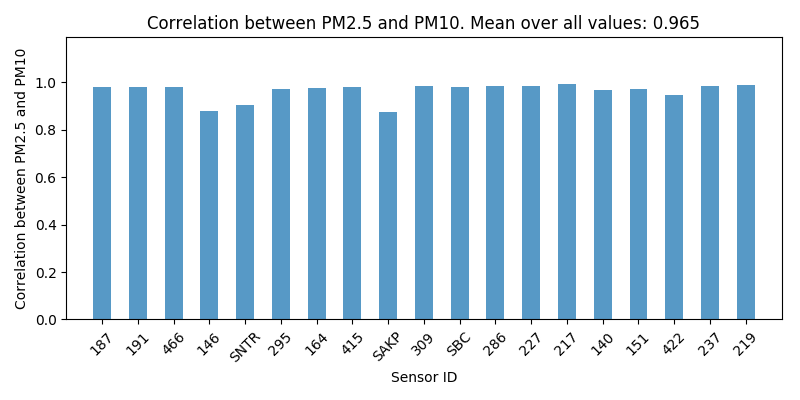
\includegraphics[width=1\textwidth]{figures/data_files_changes/1D_P1_P2_correlation}}
        \caption[PM2.5-PM10 correlation (one day average)]{PM2.5-PM10 correlation in the daily averaged data}
      \end{figure}
      \begin{figure}[H]
        \centerline{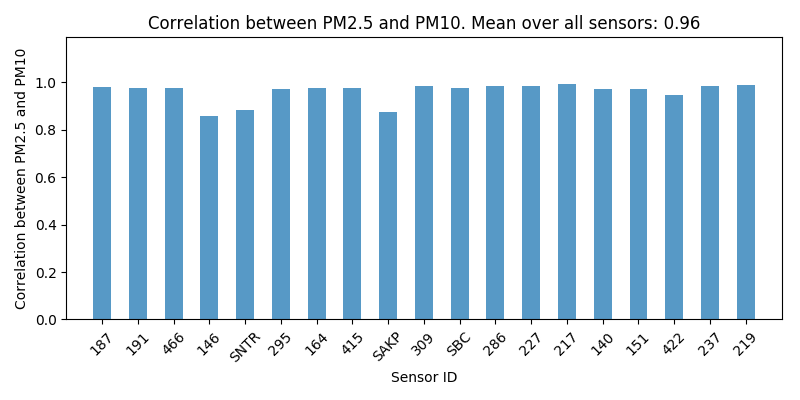
\includegraphics[width=1\textwidth]{figures/data_files_changes/12H_P1_P2_correlation}}
        \caption[PM2.5-PM10 correlation (twelve hour average)]{PM2.5-PM10 correlation in the twelve hourly averaged data}
      \end{figure}
      \begin{figure}[H]
        \centerline{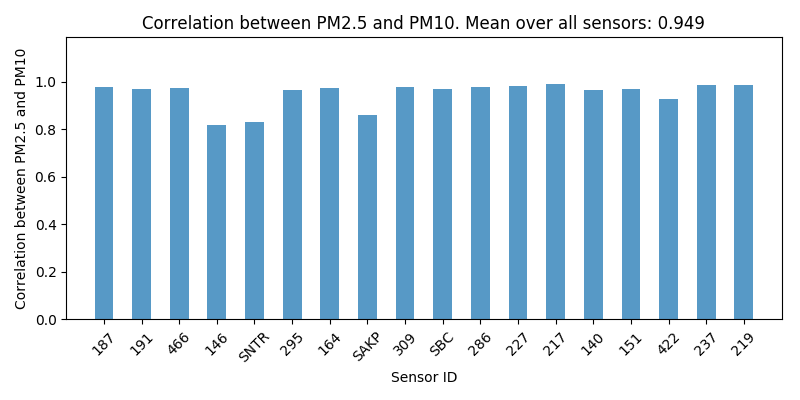
\includegraphics[width=1\textwidth]{figures/data_files_changes/1H_P1_P2_correlation}}
        \caption[PM2.5-PM10 correlation (one hour average)]{PM2.5-PM10 correlation in the hourly averaged data}
      \end{figure}  
    \end{center}
    
    \clearpage
    \chapter{Data Metrics changes}\label{app:b}
    In this appendix we present plots outlining how the used data was changed during the preprocessing. We compare several statistical metrics of the values of all sensors before and after the applied techniques for missing data filling. The techniques are described in \refsec{sec:desc-module}. We examine the data from different averaging periods in separate sets of plots. The considered metrics are minimum value, maximum value, mean value and standard deviation.
    \begin{center}
      \begin{figure}[h!] \centerline{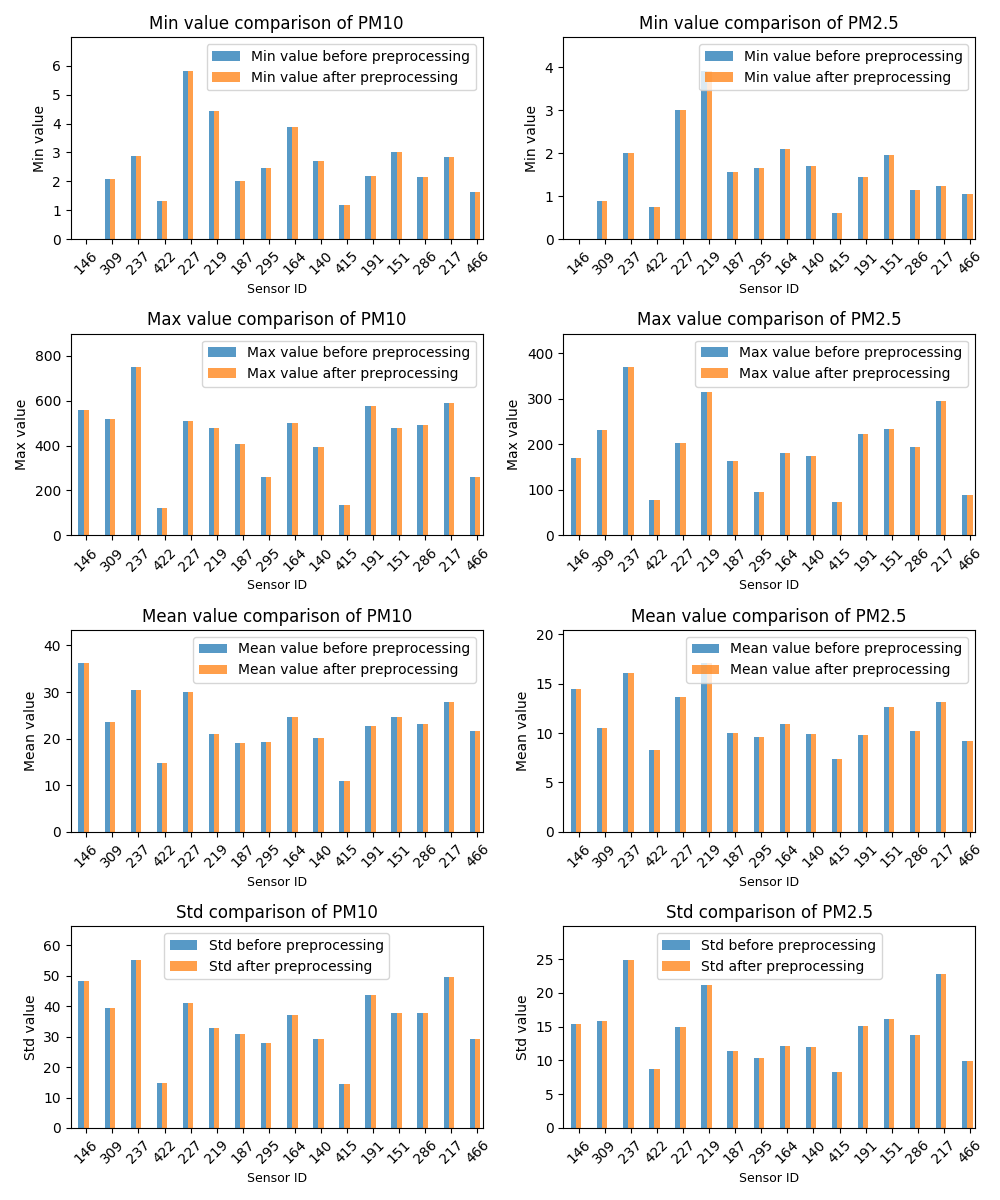
\includegraphics[width=1.1\textwidth,height=1.1\textwidth]{figures/data_files_changes/1D_sensor_metrics}}
        \caption[Metrics change during preprocessing (one day average)]{Daily average}
      \end{figure}

      \begin{figure}[H]
        \centerline{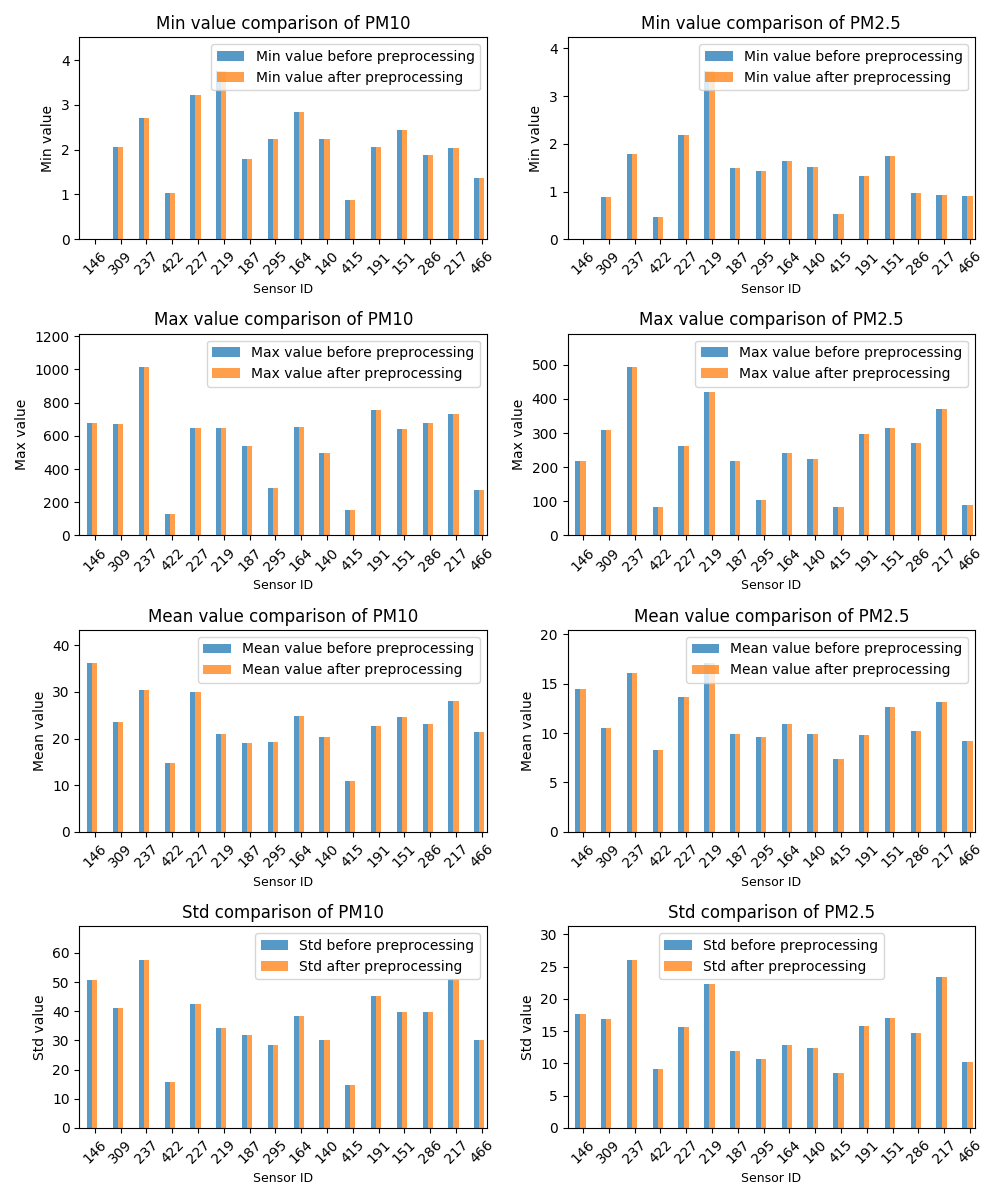
\includegraphics[width=1.1\textwidth,height=1.3\textwidth]{figures/data_files_changes/12H_sensor_metrics}}
        \caption[Metrics change during preprocessing (twelve hour average)]{Twelve hour average}
      \end{figure}

      \begin{figure}[H]
        \centerline{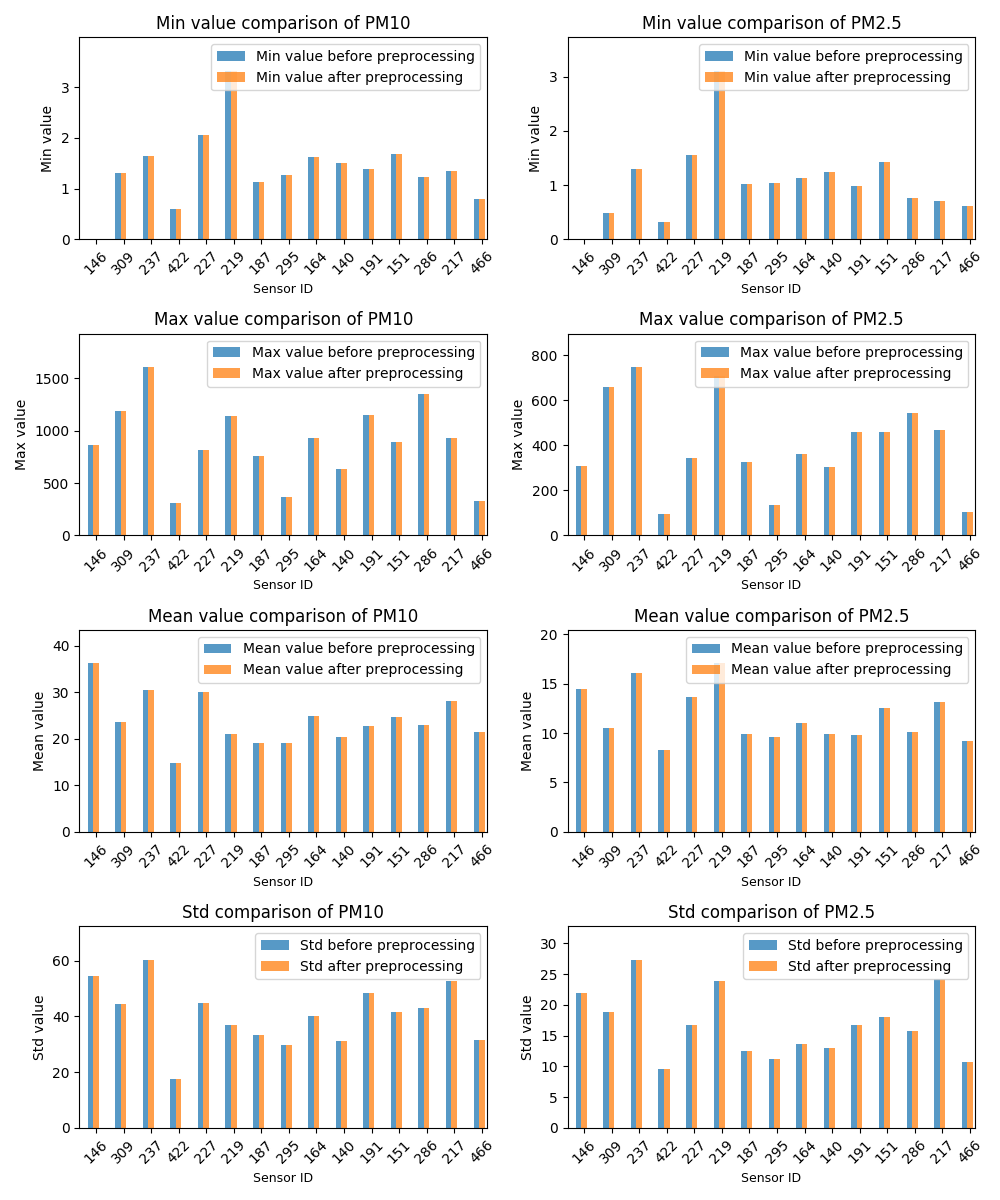
\includegraphics[width=1.1\textwidth,height=1.3\textwidth]{figures/data_files_changes/1H_sensor_metrics}}
        \caption[Metrics change during preprocessing (one hour average)]{One hour average}
      \end{figure}
      
    \end{center}
    \clearpage
    \chapter{LS and DSS scores plots}\label{app:c}
    In this appendix we present the summarizing plots of the LS- and DSS-scoring rules over the models. The plots here are analogous to the ones with the CRPS shown in \refsec{sec:res-1d}, \refsec{sec:res-12h} and \refsec{sec:res-1h}.
    \begin{figure}[h!]
      \centering
      \begin{subfigure}[t]{0.49\textwidth}
        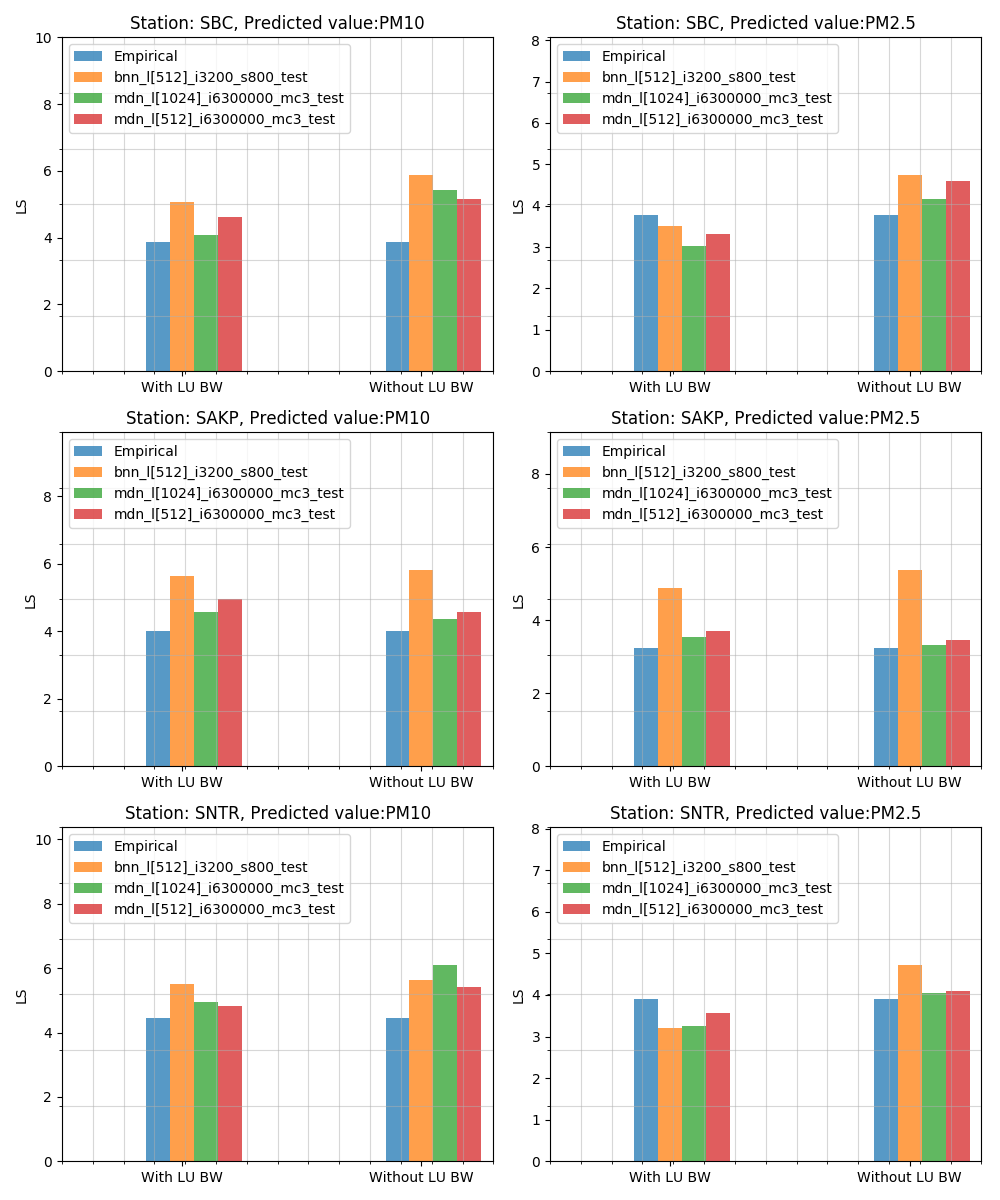
\includegraphics[width=\textwidth,height=1.2\textwidth]{figures/figs_1d/results_plot_LS}%
        \caption{Logarithmic scores}
      \end{subfigure}
      %%%%%%%%%%%%%%%%%%%%%%%%%%%%%%%%%%%%%%%%%%%%%%%%%%% 
      \begin{subfigure}[t]{0.49\textwidth}
        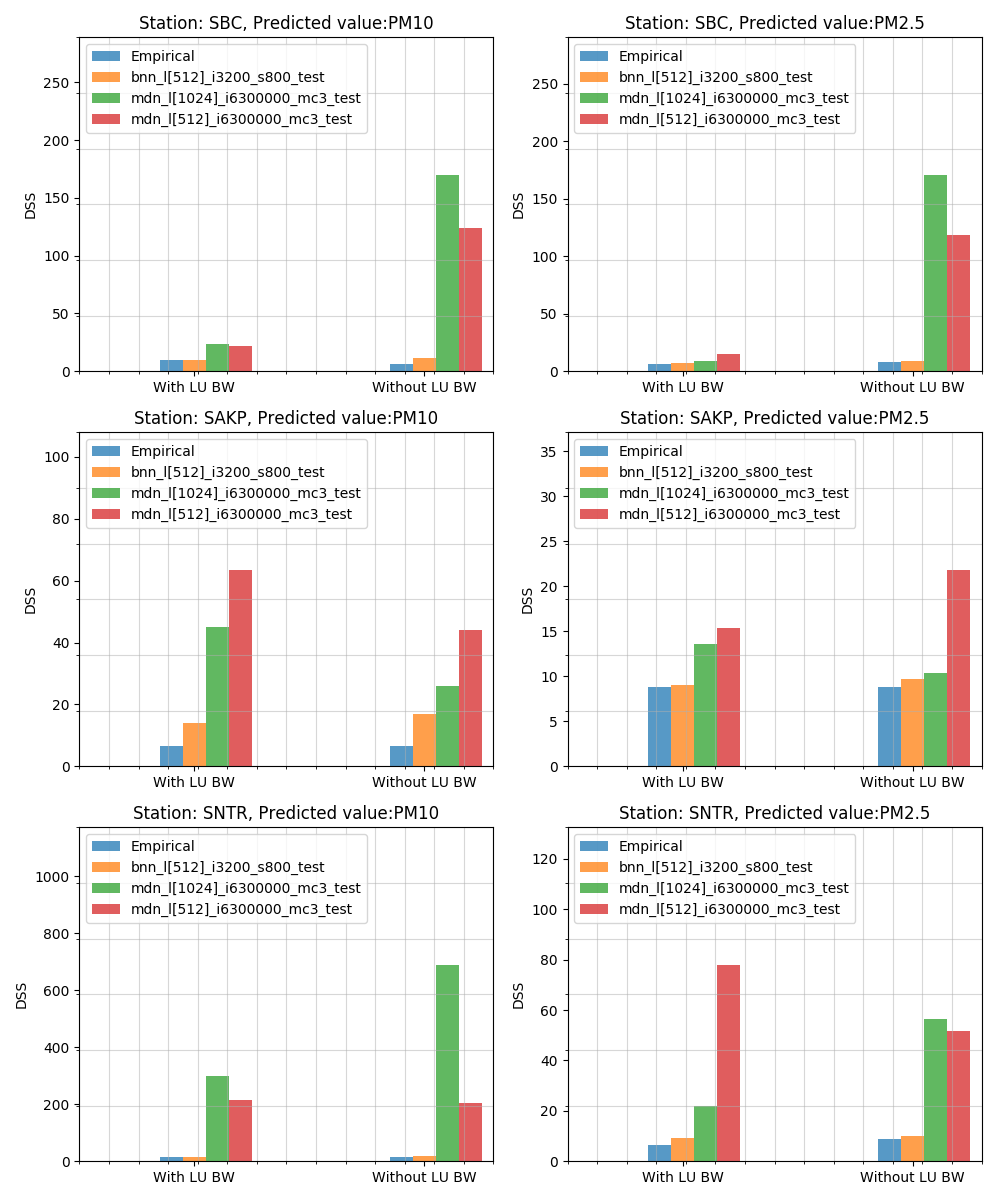
\includegraphics[width=\textwidth,height=1.2\textwidth]{figures/figs_1d/results_plot_DSS}%
        \caption{Dawid–Sebastiani scores}
      \end{subfigure}
      \caption[DSS and LS of the models (daily averaged data)]{DSS and LS values of the models trained with daily averaged data.}
    \end{figure}
    \begin{figure}[h!]
      \centering
      \begin{subfigure}[t]{0.49\textwidth}
        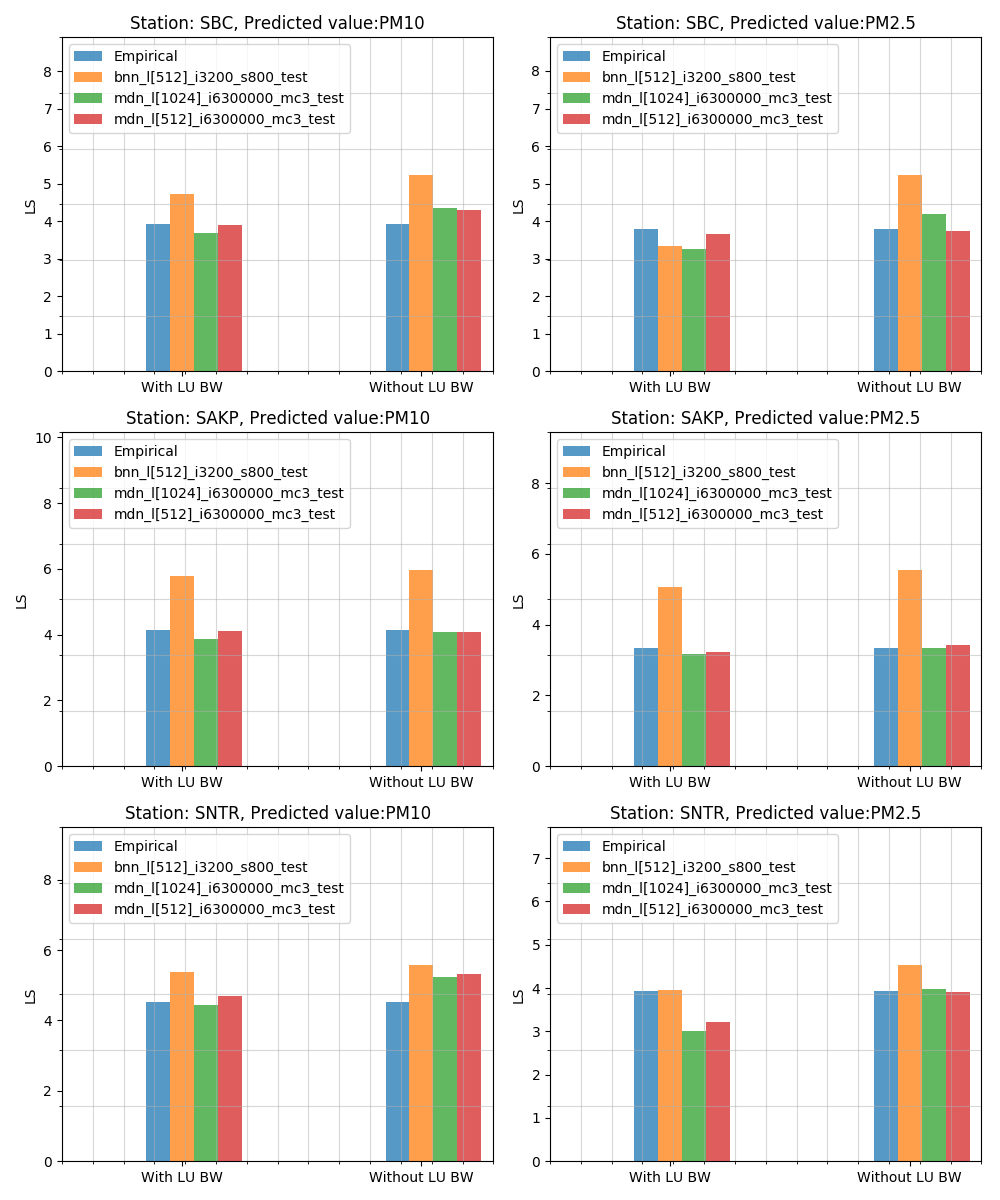
\includegraphics[width=\textwidth,height=1.2\textwidth]{figures/figs_12h/results_plot_LS}%
        \caption{Logarithmic scores}
      \end{subfigure}
      %%%%%%%%%%%%%%%%%%%%%%%%%%%%%%%%%%%%%%%%%%%%%%%%%%% 
      \begin{subfigure}[t]{0.49\textwidth}
        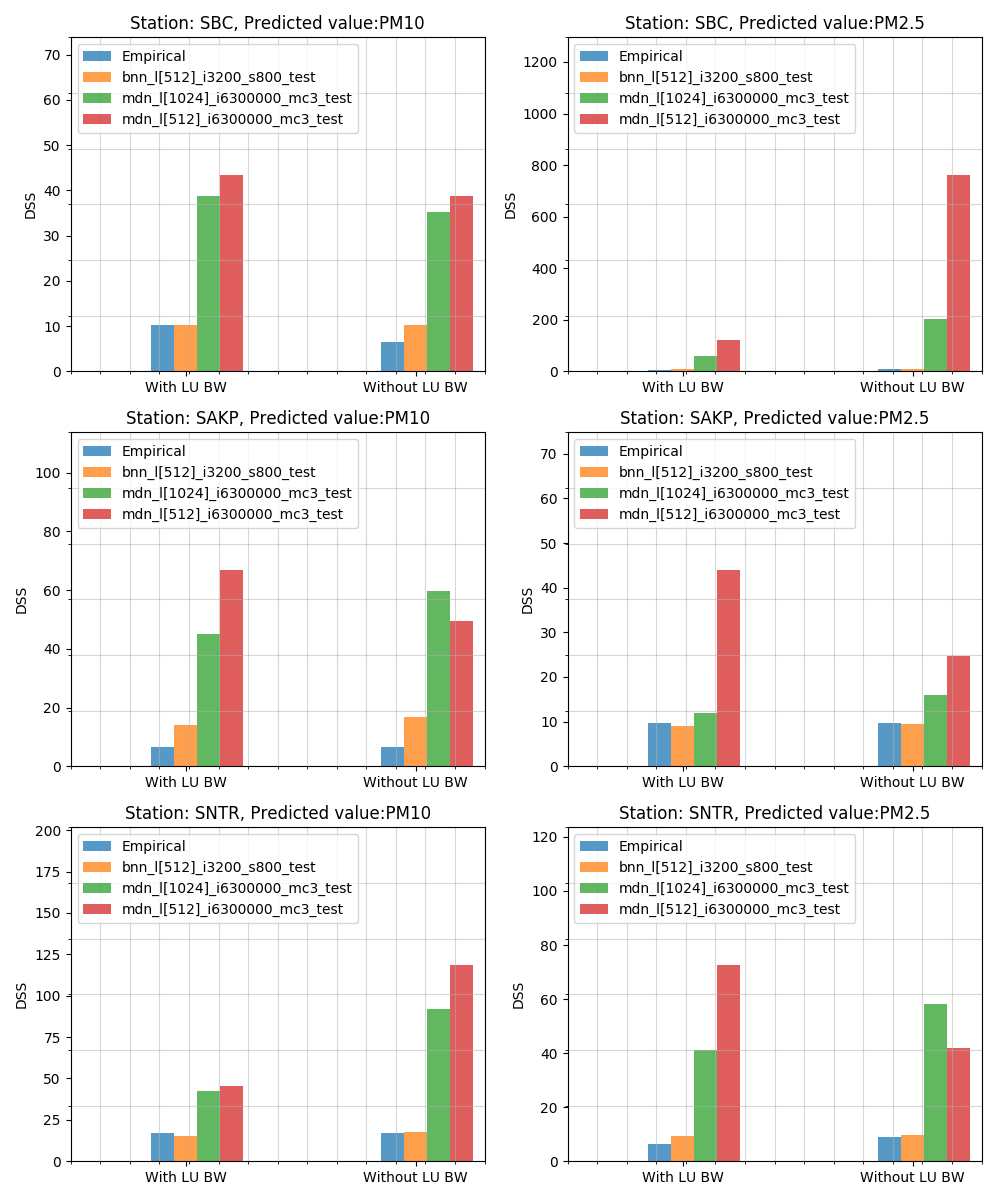
\includegraphics[width=\textwidth,height=1.2\textwidth]{figures/figs_12h/results_plot_DSS}%
        \caption{Dawid–Sebastiani scores}
      \end{subfigure}
      \caption[DSS and LS of the models (twelve hourly averaged data)]{DSS and LS values of the models trained with twelve hourly averaged data.}
    \end{figure}
    \begin{figure}[h!]
      \centering
      \begin{subfigure}[t]{0.49\textwidth}
        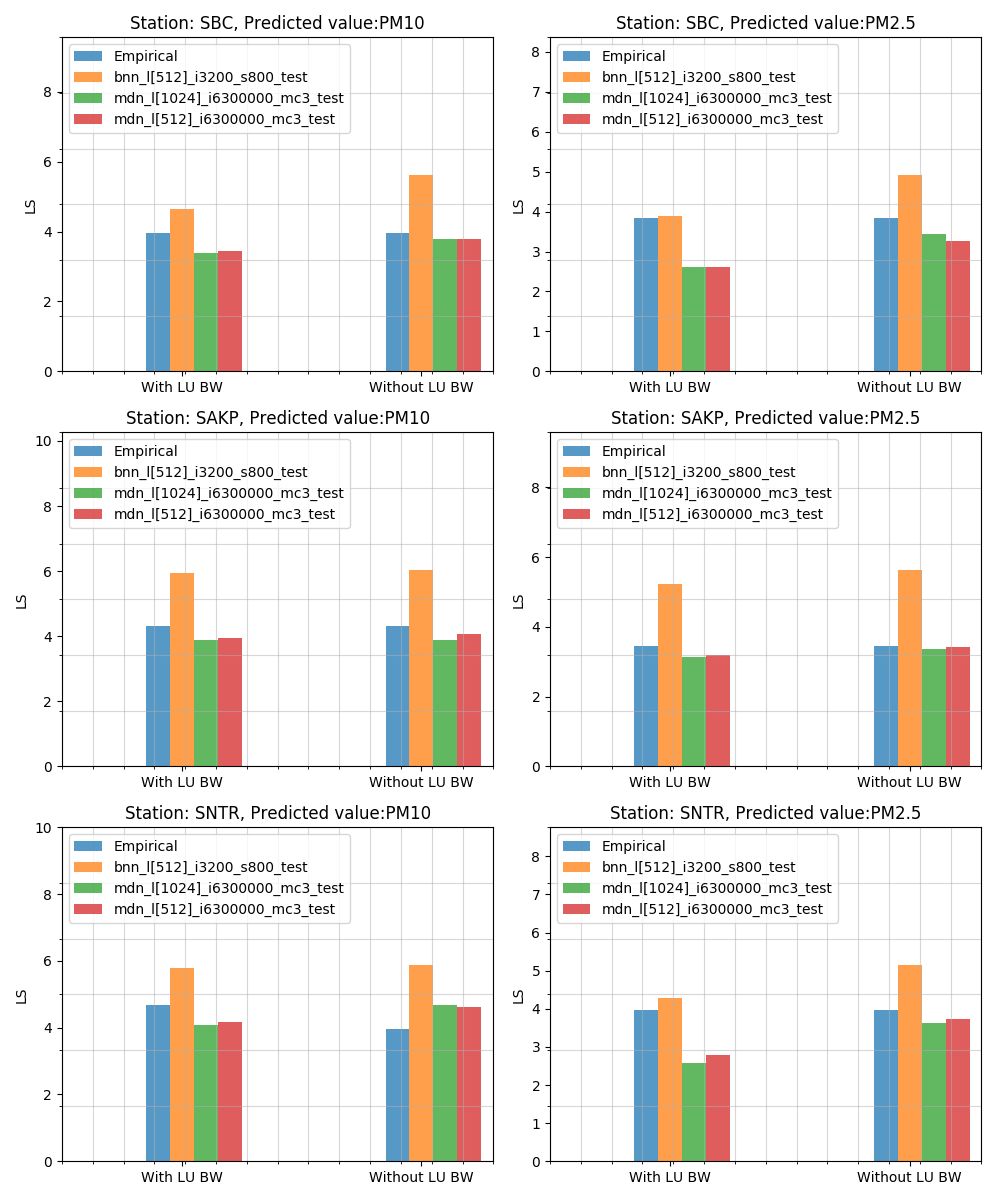
\includegraphics[width=\textwidth,height=1.2\textwidth]{figures/figs_1h/results_plot_LS}%
        \caption{Logarithmic scores}
      \end{subfigure}
      %%%%%%%%%%%%%%%%%%%%%%%%%%%%%%%%%%%%%%%%%%%%%%%%%%% 
      \begin{subfigure}[t]{0.49\textwidth}
        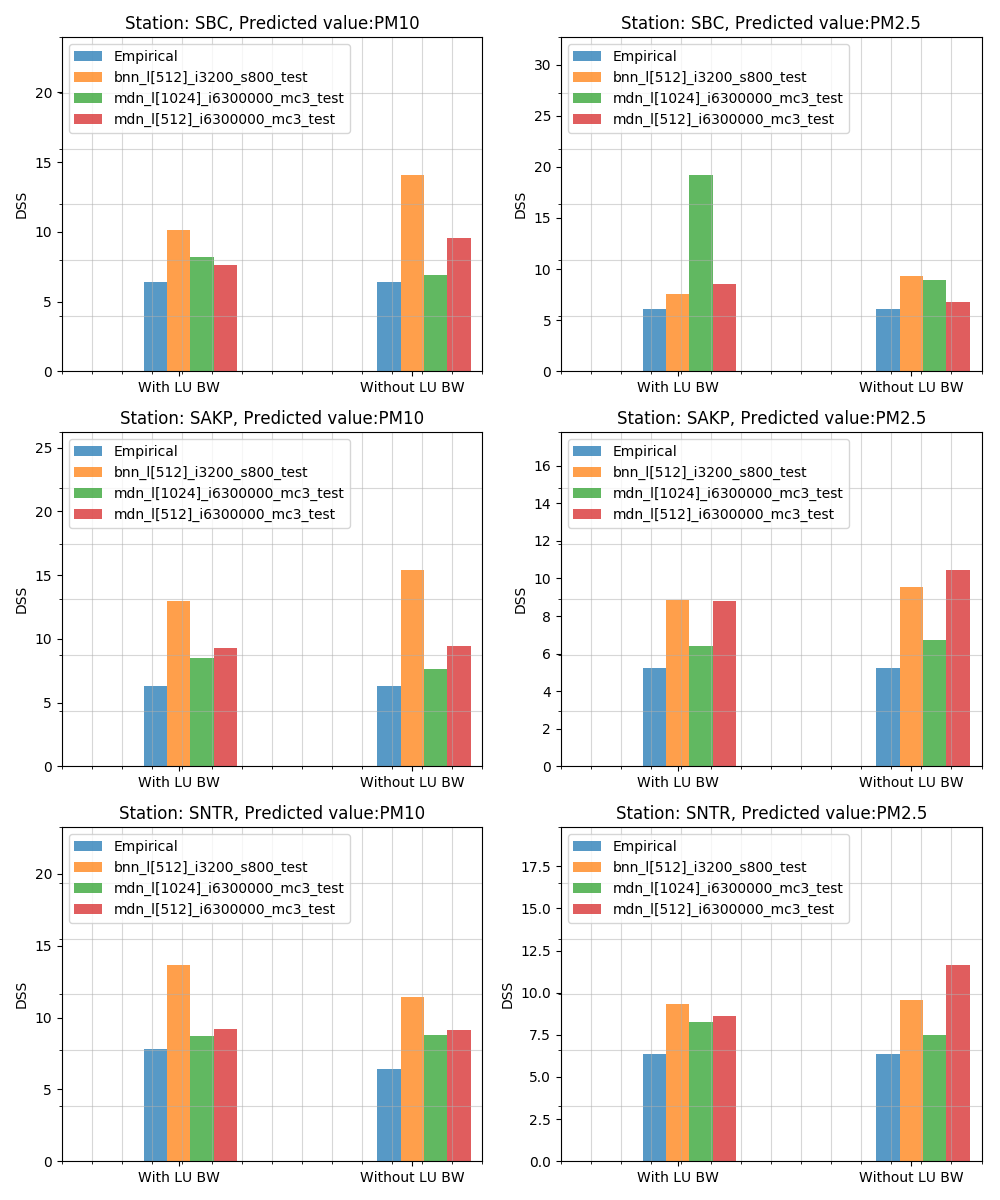
\includegraphics[width=\textwidth,height=1.2\textwidth]{figures/figs_1h/results_plot_DSS}%
        \caption{Dawid–Sebastiani scores}
      \end{subfigure}
      \caption[DSS and LS of the models (hourly averaged data)]{DSS and LS values of the models trained with hourly averaged data.}
    \end{figure}

    

    \clearpage
    \chapter{Results tables}\label{app:d}
    In this appendix we summarize the results shown with the plots in \refsec{sec:eval-model} by giving them in tabular form. We give three tables, one for each averaging period of the data used. The respective tables are \reftab{tab:res-1d}, \reftab{tab:res-12h} and \reftab{tab:res-1h}.

    The tables are split rowwise in three sections for each of the scoring rules - CRPS, DSS, LS. Each row in these sections is a separate model. The type of the data that was used to train each models is given through the titles of the corresponding columns. The ``with LUBW'' implies that the corresponding model uses values of LUBW-senors as features whereas ``without LUBW'' implies the opposite.

    All of the values are calculate based on the performance of the models on the test set of the used data.
    
    \begin{sidewaystable}
      \centering
      \captionsetup{width=0.7\linewidth,justification=raggedright}
    \begin{tabular}{c V{2.6}c V{0.3}cc||cc||cc||cc||cc||cc} 
    \hline 
    \hline 
    && \multicolumn{2}{c||}{SBC PM10}& \multicolumn{2}{c||}{SBC PM2.5}& \multicolumn{2}{c||}{SNTR PM10}& \multicolumn{2}{c||}{SNTR PM2.5}&\multicolumn{2}{c||}{SAKP PM10}& \multicolumn{2}{c}{SAKP PM2.5}\\ 
    \Xhline{2.3\arrayrulewidth} 
    &&with&without&with&without&with&without&with&without&with&without&with&without\\ 
    &&LUBW&LUBW&LUBW&LUBW&LUBW&LUBW&LUBW&LUBW&LUBW&LUBW&LUBW&LUBW\\ 
    \Xhline{2.6\arrayrulewidth} 
    CRPS&&&&&&&&&&&\\ 
    &Emp.&6.451&6.451&5.482&5.481&11.645&11.65&6.199&6.203&5.891&5.888&3.585&3.586\\ 
    &BNN$_1$&5.565&9.558&2.186&5.727&8.863&12.417&3.362&5.004&7.34&7.518&4.086&4.401\\ 
    &MDN$_1$&4.115&4.86&1.743&4.278&9.505&10.163&1.903&4.242&5.935&5.577&2.928&3.311\\ 
    &MDN$_2$&4.722&5.138&2.008&4.76&16.477&11.291&2.206&4.367&6.814&5.83&2.978&3.363\\ 
    \Xhline{2.6\arrayrulewidth} 
    LS&&&&&&&&&&&\\ 
    &Emp.&3.916&3.916&3.794&3.793&4.515&4.515&3.931&3.932&4.15&4.148&3.345&3.346\\ 
    &BNN$_1$&4.723&5.236&3.351&5.233&5.379&5.58&3.949&4.535&5.793&5.972&5.068&5.548\\ 
    &MDN$_1$&3.678&4.353&3.258&4.193&4.442&5.226&3.007&3.98&3.882&4.068&3.158&3.349\\ 
    &MDN$_2$&3.902&4.306&3.644&3.738&4.693&5.33&3.209&3.912&4.116&4.068&3.227&3.416\\ 
    \Xhline{2.6\arrayrulewidth} 
    DSS&&&&&&&&&&&\\ 
        &Emp.&10.308&6.385&6.008&8.588&16.816&16.838&6.338&9.047&6.433&6.433&9.777&9.778\\ 
    &BNN$_1$&10.319&10.267&8.266&7.828&15.233&17.845&9.246&9.604&13.905&16.741&8.912&9.559\\ 
    &MDN$_1$&38.828&35.154&59.36&201.865&42.364&91.931&41.296&58.132&45.138&59.779&11.901&16.055\\ 
    &MDN$_2$&43.439&38.79&121.177&762.176&45.287&118.649&72.676&41.84&66.884&49.566&44.0&24.608\\ 
    \Xhline{2.6\arrayrulewidth} 
  \end{tabular} 
  \captionof{table}{Table with results from scoring rules over models trained with twelve hourly averaged data.\\Emp. : \texttt{Empirical} \\ BNN$_1$ : \texttt{bnn\_l[512]\_i3200\_s800\_test} \\ MDN$_1$ : \texttt{mdn\_l[1024]\_i6300000\_mc3\_test} \\ MDN$_2$ : \texttt{mdn\_l[512]\_i6300000\_mc3\_test} }\label{tab:res-1d}
    \end{sidewaystable}

    \begin{sidewaystable}
      \centering
      \captionsetup{width=0.7\linewidth,justification=raggedright}
    \begin{tabular}{c V{2.6}c V{0.3}cc||cc||cc||cc||cc||cc} 
    \hline 
    \hline 
    && \multicolumn{2}{c||}{SBC PM10}& \multicolumn{2}{c||}{SBC PM2.5}& \multicolumn{2}{c||}{SNTR PM10}& \multicolumn{2}{c||}{SNTR PM2.5}&\multicolumn{2}{c||}{SAKP PM10}& \multicolumn{2}{c}{SAKP PM2.5}\\ 
    \Xhline{2.3\arrayrulewidth} 
    &&with&without&with&without&with&without&with&without&with&without&with&without\\ 
    &&LUBW&LUBW&LUBW&LUBW&LUBW&LUBW&LUBW&LUBW&LUBW&LUBW&LUBW&LUBW\\ 
    \Xhline{2.6\arrayrulewidth} 
    CRPS&&&&&&&&&&&\\ 
    &Emp.&6.451&6.451&5.482&5.481&11.645&11.65&6.199&6.203&5.891&5.888&3.585&3.586\\ 
    &BNN$_1$&5.565&9.558&2.186&5.727&8.863&12.417&3.362&5.004&7.34&7.518&4.086&4.401\\ 
    &MDN$_1$&4.115&4.86&1.743&4.278&9.505&10.163&1.903&4.242&5.935&5.577&2.928&3.311\\ 
    &MDN$_2$&4.722&5.138&2.008&4.76&16.477&11.291&2.206&4.367&6.814&5.83&2.978&3.363\\ 
    \Xhline{2.6\arrayrulewidth} 
    LS&&&&&&&&&&&\\ 
    &Emp.&3.916&3.916&3.794&3.793&4.515&4.515&3.931&3.932&4.15&4.148&3.345&3.346\\ 
    &BNN$_1$&4.723&5.236&3.351&5.233&5.379&5.58&3.949&4.535&5.793&5.972&5.068&5.548\\ 
    &MDN$_1$&3.678&4.353&3.258&4.193&4.442&5.226&3.007&3.98&3.882&4.068&3.158&3.349\\ 
    &MDN$_2$&3.902&4.306&3.644&3.738&4.693&5.33&3.209&3.912&4.116&4.068&3.227&3.416\\ 
    \Xhline{2.6\arrayrulewidth} 
    DSS&&&&&&&&&&&\\ 
        &Emp.&10.308&6.385&6.008&8.588&16.816&16.838&6.338&9.047&6.433&6.433&9.777&9.778\\ 
    &BNN$_1$&10.319&10.267&8.266&7.828&15.233&17.845&9.246&9.604&13.905&16.741&8.912&9.559\\ 
    &MDN$_1$&38.828&35.154&59.36&201.865&42.364&91.931&41.296&58.132&45.138&59.779&11.901&16.055\\ 
    &MDN$_2$&43.439&38.79&121.177&762.176&45.287&118.649&72.676&41.84&66.884&49.566&44.0&24.608\\ 
    \Xhline{2.6\arrayrulewidth} 
  \end{tabular} 
  \captionof{table}{Table with results from scoring rules over models trained with twelve hourly averaged data.\\Emp. : \texttt{Empirical} \\ BNN$_1$ : \texttt{bnn\_l[512]\_i3200\_s800\_test} \\ MDN$_1$ : \texttt{mdn\_l[1024]\_i6300000\_mc3\_test} \\ MDN$_2$ : \texttt{mdn\_l[512]\_i6300000\_mc3\_test} }\label{tab:res-12h}
    \end{sidewaystable}

    \begin{sidewaystable}
      \centering
      \captionsetup{width=0.7\linewidth,justification=raggedright}
    \begin{tabular}{c V{2.6}c V{0.3}cc||cc||cc||cc||cc||cc} 
    \hline 
    \hline 
    && \multicolumn{2}{c||}{SBC PM10}& \multicolumn{2}{c||}{SBC PM2.5}& \multicolumn{2}{c||}{SNTR PM10}& \multicolumn{2}{c||}{SNTR PM2.5}&\multicolumn{2}{c||}{SAKP PM10}& \multicolumn{2}{c}{SAKP PM2.5}\\ 
    \Xhline{2.3\arrayrulewidth} 
    &&with&without&with&without&with&without&with&without&with&without&with&without\\ 
    &&LUBW&LUBW&LUBW&LUBW&LUBW&LUBW&LUBW&LUBW&LUBW&LUBW&LUBW&LUBW\\ 
    \Xhline{2.6\arrayrulewidth} 
    CRPS&&&&&&&&&&&\\ 
    &Emp.&6.451&6.451&5.482&5.481&11.645&11.65&6.199&6.203&5.891&5.888&3.585&3.586\\ 
    &BNN$_1$&5.565&9.558&2.186&5.727&8.863&12.417&3.362&5.004&7.34&7.518&4.086&4.401\\ 
    &MDN$_1$&4.115&4.86&1.743&4.278&9.505&10.163&1.903&4.242&5.935&5.577&2.928&3.311\\ 
    &MDN$_2$&4.722&5.138&2.008&4.76&16.477&11.291&2.206&4.367&6.814&5.83&2.978&3.363\\ 
    \Xhline{2.6\arrayrulewidth} 
    LS&&&&&&&&&&&\\ 
    &Emp.&3.916&3.916&3.794&3.793&4.515&4.515&3.931&3.932&4.15&4.148&3.345&3.346\\ 
    &BNN$_1$&4.723&5.236&3.351&5.233&5.379&5.58&3.949&4.535&5.793&5.972&5.068&5.548\\ 
    &MDN$_1$&3.678&4.353&3.258&4.193&4.442&5.226&3.007&3.98&3.882&4.068&3.158&3.349\\ 
    &MDN$_2$&3.902&4.306&3.644&3.738&4.693&5.33&3.209&3.912&4.116&4.068&3.227&3.416\\ 
    \Xhline{2.6\arrayrulewidth} 
    DSS&&&&&&&&&&&\\ 
        &Emp.&10.308&6.385&6.008&8.588&16.816&16.838&6.338&9.047&6.433&6.433&9.777&9.778\\ 
    &BNN$_1$&10.319&10.267&8.266&7.828&15.233&17.845&9.246&9.604&13.905&16.741&8.912&9.559\\ 
    &MDN$_1$&38.828&35.154&59.36&201.865&42.364&91.931&41.296&58.132&45.138&59.779&11.901&16.055\\ 
    &MDN$_2$&43.439&38.79&121.177&762.176&45.287&118.649&72.676&41.84&66.884&49.566&44.0&24.608\\ 
    \Xhline{2.6\arrayrulewidth} 
  \end{tabular} 
  \captionof{table}{Table with results from scoring rules over models trained with twelve hourly averaged data.\\Emp. : \texttt{Empirical} \\ BNN$_1$ : \texttt{bnn\_l[512]\_i3200\_s800\_test} \\ MDN$_1$ : \texttt{mdn\_l[1024]\_i6300000\_mc3\_test} \\ MDN$_2$ : \texttt{mdn\_l[512]\_i6300000\_mc3\_test} }\label{tab:res-1h}
    \end{sidewaystable}
    \clearpage
    \chapter{Predictive performance checks results tables}\label{app:e}
    In this appendix we give tables with the results of the predictive performance checks over the models, as mentioned in \refsec{sec:preprop-meth}. We again give three separate tables for the three averaging periods. The tables are \reftab{tab:pred-1d}, \reftab{tab:pred-12h} and \reftab{tab:pred-1h}. The format compares every pair of models. We only consider models that predict the PM10 value of each LUBW sensor and the predictive performance check is calculated with respect to the CRPS.
    
    The tables are split rowwise in three big sections for each LUBW-station -- \textbf{SBC}, \textbf{SNTR}, \textbf{SAKP}. Each of these sections is further divided in two smaller ones in which we consider models trained either with or without the use of values from the other two LUBW-stations as features. The column-wise division is only based on the latter consideration. This defines grid of columns and rows where in each column and each row represents a model trained e certain way. At the cell where two models intersect, we give the value of the predictive performance check between them. It is important to note that the predicted station of each column model chages depending on the context in which it is compared. For example, the first column model predicts values of SBC when compared with models from the \textbf{SBC} section of the table but it predicts values of SNTR when compared with models from the \textbf{SNTR} section of the table. The names of the models are given through aliases that are explained in the caption of each table.
    
    The values given in the tables are the actual metric of the Diebold-Mariano test. The marked with start (\(^* \)) entries are the ones that we consider as statistically significant. For these entries the corresponding \(p\)-value is smaller than \(0.05\). If the given metric is negative, the model in the corresponding row is considered better with respect to its predictive capabilities. If the metric is positive -- the model in the corresponding column is to be considered as the better one.

    All of the values are calculate based on the performance of the models on the test set of the used data.
    \begin{sidewaystable}
      \centering
      \begin{tabular}{c|c|cccc||cccc} 
  \hline 
  \hline 
  &&\multicolumn{3}{c}{PM10 with LUBW} && \multicolumn{3}{c}{PM10 without LUBW} \\ 
  \hline 
  &&Emp.&BNN$_1$&MDN$_1$&MDN$_2$&Emp.&BNN$_1$&MDN$_1$&MDN$_2$ \\ 
  \hline 
  \hline 
  \textbf{SBC}&&&&&&& \\ 
  PM10&Emp.&\texttt{\--}&1.44&4.73$^*$&3.62$^*$&\texttt{\--}&\texttt{\--}&\texttt{\--}&\texttt{\--} \\ 
  with&BNN$_1$&-1.44&\texttt{\--}&4.13$^*$&1.66&\texttt{\--}&\texttt{\--}&\texttt{\--}&\texttt{\--} \\ 
  LUBW&MDN$_1$&-4.73$^*$&-4.13$^*$&\texttt{\--}&-4.08$^*$&\texttt{\--}&\texttt{\--}&\texttt{\--}&\texttt{\--} \\ 
  &MDN$_2$&-3.62$^*$&-1.66&4.08$^*$&\texttt{\--}&\texttt{\--}&\texttt{\--}&\texttt{\--}&\texttt{\--} \\ 
  \hline     
  PM10&Emp.&\texttt{\--}&\texttt{\--}&\texttt{\--}&\texttt{\--}&\texttt{\--}&-2.88$^*$&-0.1&-0.92 \\ 
  without&BNN$_1$&\texttt{\--}&\texttt{\--}&\texttt{\--}&\texttt{\--}&2.88$^*$&\texttt{\--}&2.9$^*$&2.89$^*$ \\ 
  LUBW&MDN$_1$&\texttt{\--}&\texttt{\--}&\texttt{\--}&\texttt{\--}&0.1&-2.9$^*$&\texttt{\--}&-1.0 \\ 
  &MDN$_2$&\texttt{\--}&\texttt{\--}&\texttt{\--}&\texttt{\--}&0.92&-2.89$^*$&1.0&\texttt{\--} \\ 
  \hline     
  \hline     
  \textbf{SNTR}&&&&&&& \\ 
  PM10&Emp.&\texttt{\--}&2.51$^*$&-1.48&0.02&\texttt{\--}&\texttt{\--}&\texttt{\--}&\texttt{\--} \\ 
  with&BNN$_1$&-2.51$^*$&\texttt{\--}&-2.73$^*$&-2.18$^*$&\texttt{\--}&\texttt{\--}&\texttt{\--}&\texttt{\--} \\ 
  LUBW&MDN$_1$&1.48&2.73$^*$&\texttt{\--}&1.5&\texttt{\--}&\texttt{\--}&\texttt{\--}&\texttt{\--} \\ 
  &MDN$_2$&-0.02&2.18$^*$&-1.5&\texttt{\--}&\texttt{\--}&\texttt{\--}&\texttt{\--}&\texttt{\--} \\ 
  \hline     
  PM10&Emp.&\texttt{\--}&\texttt{\--}&\texttt{\--}&\texttt{\--}&\texttt{\--}&-1.01&0.43&0.87 \\ 
  without&BNN$_1$&\texttt{\--}&\texttt{\--}&\texttt{\--}&\texttt{\--}&1.01&\texttt{\--}&1.28&1.51 \\ 
  LUBW&MDN$_1$&\texttt{\--}&\texttt{\--}&\texttt{\--}&\texttt{\--}&-0.43&-1.28&\texttt{\--}&1.42 \\ 
  &MDN$_2$&\texttt{\--}&\texttt{\--}&\texttt{\--}&\texttt{\--}&-0.87&-1.51&-1.42&\texttt{\--} \\ 
  \hline     
  \hline     
  \textbf{SAKP}&&&&&&& \\ 
  PM10&Emp.&\texttt{\--}&-6.94$^*$&-2.21$^*$&-2.37$^*$&\texttt{\--}&\texttt{\--}&\texttt{\--}&\texttt{\--} \\ 
  with&BNN$_1$&6.94$^*$&\texttt{\--}&-2.2$^*$&-2.35$^*$&\texttt{\--}&\texttt{\--}&\texttt{\--}&\texttt{\--} \\ 
  LUBW&MDN$_1$&2.21$^*$&2.2$^*$&\texttt{\--}&0.57&\texttt{\--}&\texttt{\--}&\texttt{\--}&\texttt{\--} \\ 
  &MDN$_2$&2.37$^*$&2.35$^*$&-0.57&\texttt{\--}&\texttt{\--}&\texttt{\--}&\texttt{\--}&\texttt{\--} \\ 
  \hline     
  PM10&Emp.&\texttt{\--}&\texttt{\--}&\texttt{\--}&\texttt{\--}&\texttt{\--}&-7.27$^*$&-2.23$^*$&-2.16$^*$ \\ 
  without&BNN$_1$&\texttt{\--}&\texttt{\--}&\texttt{\--}&\texttt{\--}&7.27$^*$&\texttt{\--}&-2.05$^*$&-2.12$^*$ \\ 
  LUBW&MDN$_1$&\texttt{\--}&\texttt{\--}&\texttt{\--}&\texttt{\--}&2.23$^*$&2.05$^*$&\texttt{\--}&-2.14$^*$ \\ 
  &MDN$_2$&\texttt{\--}&\texttt{\--}&\texttt{\--}&\texttt{\--}&2.16$^*$&2.12$^*$&2.14$^*$&\texttt{\--} \\ 
  \hline     
  \hline     
\end{tabular}
\captionof{table}{Table with results of predictive checks between models trained with daily averaged data.\\Emp. : \texttt{Empirical} \\ BNN$_1$ : \texttt{bnn\_l[512]\_i3200\_s800\_test} \\ MDN$_1$ : \texttt{mdn\_l[1024]\_i6300000\_mc3\_testl}\\ MDN$_2$ : \texttt{mdn\_l[512]\_i6300000\_mc3\_testl} }\label{tab:pred-1d}
    \end{sidewaystable}
    \begin{sidewaystable}
      \centering
      \begin{tabular}{c|c|cccc||cccc} 
  \hline 
  \hline 
  &&\multicolumn{3}{c}{PM10 with LUBW} && \multicolumn{3}{c}{PM10 without LUBW} \\ 
  \hline 
  &&Emp.&BNN$_1$&MDN$_1$&MDN$_2$&Emp.&BNN$_1$&MDN$_1$&MDN$_2$ \\ 
  \hline 
  \hline 
  \textbf{SBC}&&&&&&& \\ 
  PM10&Emp.&\texttt{\--}&1.44&4.73$^*$&3.62$^*$&\texttt{\--}&\texttt{\--}&\texttt{\--}&\texttt{\--} \\ 
  with&BNN$_1$&-1.44&\texttt{\--}&4.13$^*$&1.66&\texttt{\--}&\texttt{\--}&\texttt{\--}&\texttt{\--} \\ 
  LUBW&MDN$_1$&-4.73$^*$&-4.13$^*$&\texttt{\--}&-4.08$^*$&\texttt{\--}&\texttt{\--}&\texttt{\--}&\texttt{\--} \\ 
  &MDN$_2$&-3.62$^*$&-1.66&4.08$^*$&\texttt{\--}&\texttt{\--}&\texttt{\--}&\texttt{\--}&\texttt{\--} \\ 
  \hline     
  PM10&Emp.&\texttt{\--}&\texttt{\--}&\texttt{\--}&\texttt{\--}&\texttt{\--}&-2.88$^*$&-0.1&-0.92 \\ 
  without&BNN$_1$&\texttt{\--}&\texttt{\--}&\texttt{\--}&\texttt{\--}&2.88$^*$&\texttt{\--}&2.9$^*$&2.89$^*$ \\ 
  LUBW&MDN$_1$&\texttt{\--}&\texttt{\--}&\texttt{\--}&\texttt{\--}&0.1&-2.9$^*$&\texttt{\--}&-1.0 \\ 
  &MDN$_2$&\texttt{\--}&\texttt{\--}&\texttt{\--}&\texttt{\--}&0.92&-2.89$^*$&1.0&\texttt{\--} \\ 
  \hline     
  \hline     
  \textbf{SNTR}&&&&&&& \\ 
  PM10&Emp.&\texttt{\--}&2.51$^*$&-1.48&0.02&\texttt{\--}&\texttt{\--}&\texttt{\--}&\texttt{\--} \\ 
  with&BNN$_1$&-2.51$^*$&\texttt{\--}&-2.73$^*$&-2.18$^*$&\texttt{\--}&\texttt{\--}&\texttt{\--}&\texttt{\--} \\ 
  LUBW&MDN$_1$&1.48&2.73$^*$&\texttt{\--}&1.5&\texttt{\--}&\texttt{\--}&\texttt{\--}&\texttt{\--} \\ 
  &MDN$_2$&-0.02&2.18$^*$&-1.5&\texttt{\--}&\texttt{\--}&\texttt{\--}&\texttt{\--}&\texttt{\--} \\ 
  \hline     
  PM10&Emp.&\texttt{\--}&\texttt{\--}&\texttt{\--}&\texttt{\--}&\texttt{\--}&-1.01&0.43&0.87 \\ 
  without&BNN$_1$&\texttt{\--}&\texttt{\--}&\texttt{\--}&\texttt{\--}&1.01&\texttt{\--}&1.28&1.51 \\ 
  LUBW&MDN$_1$&\texttt{\--}&\texttt{\--}&\texttt{\--}&\texttt{\--}&-0.43&-1.28&\texttt{\--}&1.42 \\ 
  &MDN$_2$&\texttt{\--}&\texttt{\--}&\texttt{\--}&\texttt{\--}&-0.87&-1.51&-1.42&\texttt{\--} \\ 
  \hline     
  \hline     
  \textbf{SAKP}&&&&&&& \\ 
  PM10&Emp.&\texttt{\--}&-6.94$^*$&-2.21$^*$&-2.37$^*$&\texttt{\--}&\texttt{\--}&\texttt{\--}&\texttt{\--} \\ 
  with&BNN$_1$&6.94$^*$&\texttt{\--}&-2.2$^*$&-2.35$^*$&\texttt{\--}&\texttt{\--}&\texttt{\--}&\texttt{\--} \\ 
  LUBW&MDN$_1$&2.21$^*$&2.2$^*$&\texttt{\--}&0.57&\texttt{\--}&\texttt{\--}&\texttt{\--}&\texttt{\--} \\ 
  &MDN$_2$&2.37$^*$&2.35$^*$&-0.57&\texttt{\--}&\texttt{\--}&\texttt{\--}&\texttt{\--}&\texttt{\--} \\ 
  \hline     
  PM10&Emp.&\texttt{\--}&\texttt{\--}&\texttt{\--}&\texttt{\--}&\texttt{\--}&-7.27$^*$&-2.23$^*$&-2.16$^*$ \\ 
  without&BNN$_1$&\texttt{\--}&\texttt{\--}&\texttt{\--}&\texttt{\--}&7.27$^*$&\texttt{\--}&-2.05$^*$&-2.12$^*$ \\ 
  LUBW&MDN$_1$&\texttt{\--}&\texttt{\--}&\texttt{\--}&\texttt{\--}&2.23$^*$&2.05$^*$&\texttt{\--}&-2.14$^*$ \\ 
  &MDN$_2$&\texttt{\--}&\texttt{\--}&\texttt{\--}&\texttt{\--}&2.16$^*$&2.12$^*$&2.14$^*$&\texttt{\--} \\ 
  \hline     
  \hline     
\end{tabular}
\captionof{table}{Table with results of predictive checks between models trained with daily averaged data.\\Emp. : \texttt{Empirical} \\ BNN$_1$ : \texttt{bnn\_l[512]\_i3200\_s800\_test} \\ MDN$_1$ : \texttt{mdn\_l[1024]\_i6300000\_mc3\_testl}\\ MDN$_2$ : \texttt{mdn\_l[512]\_i6300000\_mc3\_testl} }\label{tab:pred-12h}
    \end{sidewaystable}
    \begin{sidewaystable}
      \centering
      \begin{tabular}{c|c|cccc||cccc} 
  \hline 
  \hline 
  &&\multicolumn{3}{c}{PM10 with LUBW} && \multicolumn{3}{c}{PM10 without LUBW} \\ 
  \hline 
  &&Emp.&BNN$_1$&MDN$_1$&MDN$_2$&Emp.&BNN$_1$&MDN$_1$&MDN$_2$ \\ 
  \hline 
  \hline 
  \textbf{SBC}&&&&&&& \\ 
  PM10&Emp.&\texttt{\--}&1.44&4.73$^*$&3.62$^*$&\texttt{\--}&\texttt{\--}&\texttt{\--}&\texttt{\--} \\ 
  with&BNN$_1$&-1.44&\texttt{\--}&4.13$^*$&1.66&\texttt{\--}&\texttt{\--}&\texttt{\--}&\texttt{\--} \\ 
  LUBW&MDN$_1$&-4.73$^*$&-4.13$^*$&\texttt{\--}&-4.08$^*$&\texttt{\--}&\texttt{\--}&\texttt{\--}&\texttt{\--} \\ 
  &MDN$_2$&-3.62$^*$&-1.66&4.08$^*$&\texttt{\--}&\texttt{\--}&\texttt{\--}&\texttt{\--}&\texttt{\--} \\ 
  \hline     
  PM10&Emp.&\texttt{\--}&\texttt{\--}&\texttt{\--}&\texttt{\--}&\texttt{\--}&-2.88$^*$&-0.1&-0.92 \\ 
  without&BNN$_1$&\texttt{\--}&\texttt{\--}&\texttt{\--}&\texttt{\--}&2.88$^*$&\texttt{\--}&2.9$^*$&2.89$^*$ \\ 
  LUBW&MDN$_1$&\texttt{\--}&\texttt{\--}&\texttt{\--}&\texttt{\--}&0.1&-2.9$^*$&\texttt{\--}&-1.0 \\ 
  &MDN$_2$&\texttt{\--}&\texttt{\--}&\texttt{\--}&\texttt{\--}&0.92&-2.89$^*$&1.0&\texttt{\--} \\ 
  \hline     
  \hline     
  \textbf{SNTR}&&&&&&& \\ 
  PM10&Emp.&\texttt{\--}&2.51$^*$&-1.48&0.02&\texttt{\--}&\texttt{\--}&\texttt{\--}&\texttt{\--} \\ 
  with&BNN$_1$&-2.51$^*$&\texttt{\--}&-2.73$^*$&-2.18$^*$&\texttt{\--}&\texttt{\--}&\texttt{\--}&\texttt{\--} \\ 
  LUBW&MDN$_1$&1.48&2.73$^*$&\texttt{\--}&1.5&\texttt{\--}&\texttt{\--}&\texttt{\--}&\texttt{\--} \\ 
  &MDN$_2$&-0.02&2.18$^*$&-1.5&\texttt{\--}&\texttt{\--}&\texttt{\--}&\texttt{\--}&\texttt{\--} \\ 
  \hline     
  PM10&Emp.&\texttt{\--}&\texttt{\--}&\texttt{\--}&\texttt{\--}&\texttt{\--}&-1.01&0.43&0.87 \\ 
  without&BNN$_1$&\texttt{\--}&\texttt{\--}&\texttt{\--}&\texttt{\--}&1.01&\texttt{\--}&1.28&1.51 \\ 
  LUBW&MDN$_1$&\texttt{\--}&\texttt{\--}&\texttt{\--}&\texttt{\--}&-0.43&-1.28&\texttt{\--}&1.42 \\ 
  &MDN$_2$&\texttt{\--}&\texttt{\--}&\texttt{\--}&\texttt{\--}&-0.87&-1.51&-1.42&\texttt{\--} \\ 
  \hline     
  \hline     
  \textbf{SAKP}&&&&&&& \\ 
  PM10&Emp.&\texttt{\--}&-6.94$^*$&-2.21$^*$&-2.37$^*$&\texttt{\--}&\texttt{\--}&\texttt{\--}&\texttt{\--} \\ 
  with&BNN$_1$&6.94$^*$&\texttt{\--}&-2.2$^*$&-2.35$^*$&\texttt{\--}&\texttt{\--}&\texttt{\--}&\texttt{\--} \\ 
  LUBW&MDN$_1$&2.21$^*$&2.2$^*$&\texttt{\--}&0.57&\texttt{\--}&\texttt{\--}&\texttt{\--}&\texttt{\--} \\ 
  &MDN$_2$&2.37$^*$&2.35$^*$&-0.57&\texttt{\--}&\texttt{\--}&\texttt{\--}&\texttt{\--}&\texttt{\--} \\ 
  \hline     
  PM10&Emp.&\texttt{\--}&\texttt{\--}&\texttt{\--}&\texttt{\--}&\texttt{\--}&-7.27$^*$&-2.23$^*$&-2.16$^*$ \\ 
  without&BNN$_1$&\texttt{\--}&\texttt{\--}&\texttt{\--}&\texttt{\--}&7.27$^*$&\texttt{\--}&-2.05$^*$&-2.12$^*$ \\ 
  LUBW&MDN$_1$&\texttt{\--}&\texttt{\--}&\texttt{\--}&\texttt{\--}&2.23$^*$&2.05$^*$&\texttt{\--}&-2.14$^*$ \\ 
  &MDN$_2$&\texttt{\--}&\texttt{\--}&\texttt{\--}&\texttt{\--}&2.16$^*$&2.12$^*$&2.14$^*$&\texttt{\--} \\ 
  \hline     
  \hline     
\end{tabular}
\captionof{table}{Table with results of predictive checks between models trained with daily averaged data.\\Emp. : \texttt{Empirical} \\ BNN$_1$ : \texttt{bnn\_l[512]\_i3200\_s800\_test} \\ MDN$_1$ : \texttt{mdn\_l[1024]\_i6300000\_mc3\_testl}\\ MDN$_2$ : \texttt{mdn\_l[512]\_i6300000\_mc3\_testl} }\label{tab:pred-1h}
    \end{sidewaystable}

    \clearpage
    \chapter{Models plots}\label{app:f}
    In this appendix we present plots that compare the predicted by the models values and the actual observations. We do not give plot for every single model. We have selected plots illustrating the predictive performance of the relatively good models. We have plotted the results of the predictions both on the training and on the test set for each plot. As with previous result considerations, we distinguish between the averaging period of the data with which the models were trained. The first two plots -- \reffig{fig:mdn-plot-1d} and \reffig{fig:bnn-plot-1d} -- show plots of models trained on daily averaged data. The next two figures -- \reffig{fig:mdn-plot-12h} and \reffig{fig:bnn-plot-12h} -- show plots from models trained on twelve hourly averaged data and final two plots -- \reffig{fig:mdn-plot-1h} and \reffig{fig:bnn-plot-1h} -- models trained on one hourly averaged data.
    \begin{center}
      \begin{figure}[h!]
        \centering
        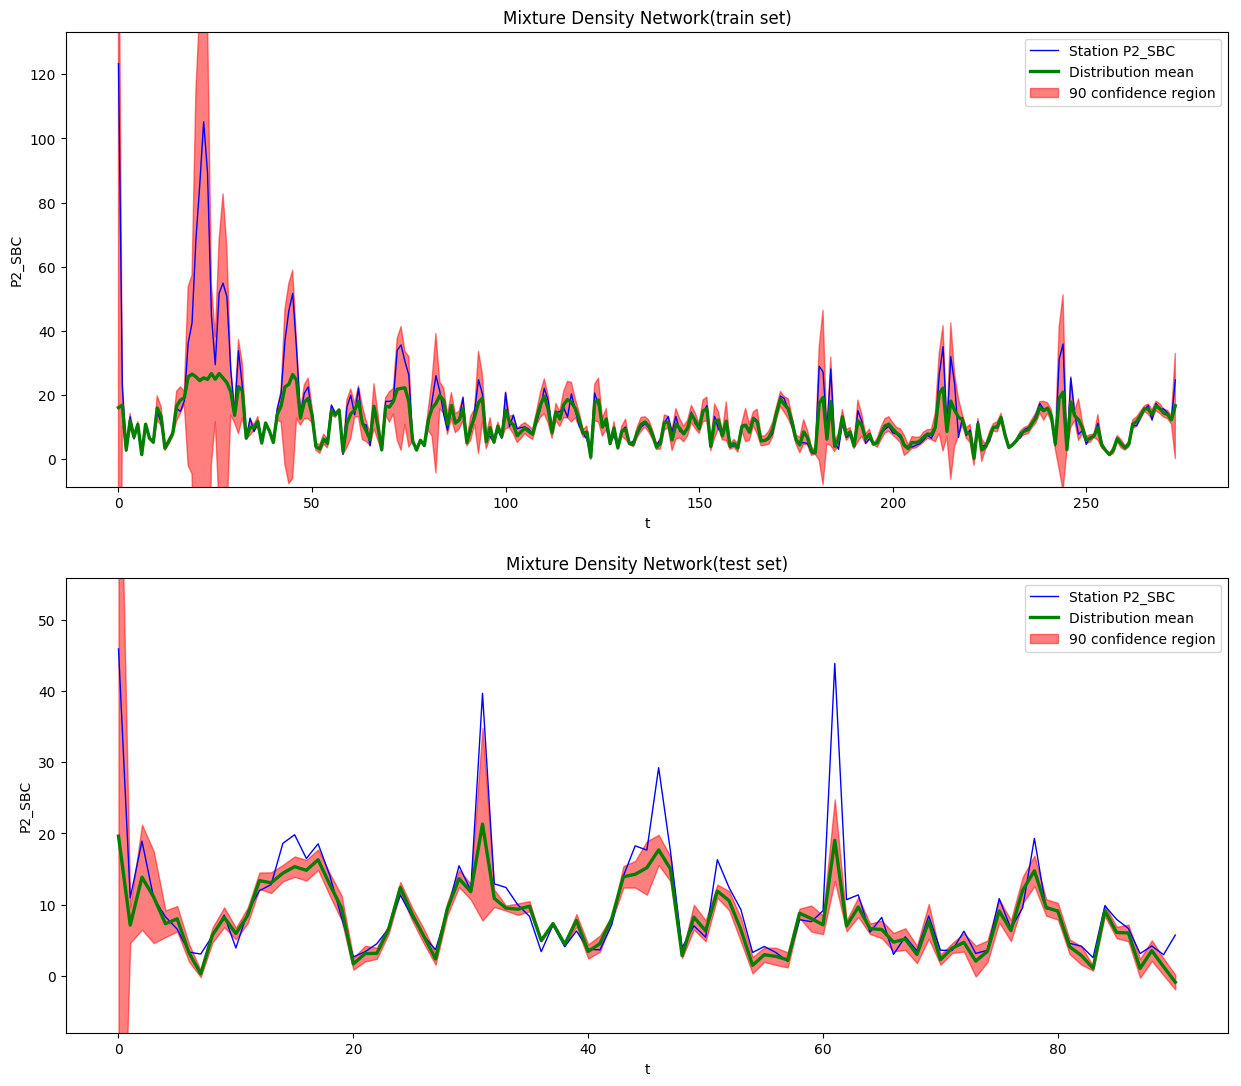
\includegraphics[height=0.75\textwidth, width=0.9\textwidth]{figures/model_plots/mdn_1d}
        \caption[MDN one day plot]{A MDN model with good performance trained on daily averaged data}\label{fig:mdn-plot-1d}
      \end{figure}
    \end{center}
    \begin{center}
      \begin{figure}[h!]
        \centering
        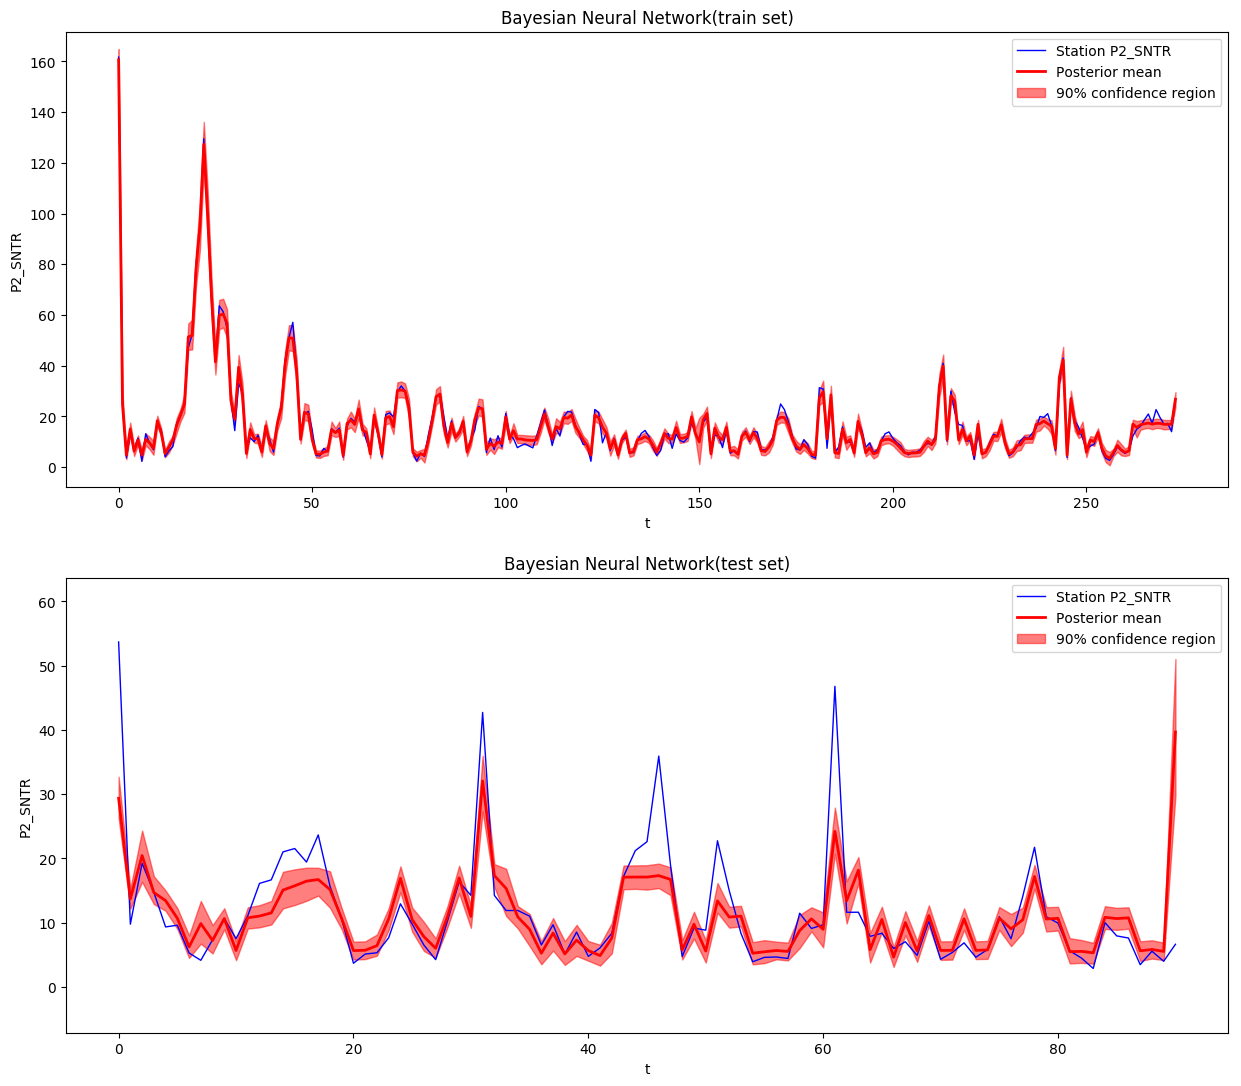
\includegraphics[height=0.6\textwidth, width=0.9\textwidth]{figures/model_plots/bnn_1d}
        \caption[BNN one day plot]{A BNN model with good performance trained on daily averaged data}\label{fig:bnn-plot-1d}
      \end{figure}
    \end{center}
    \begin{center}
      \begin{figure}[h!]
        \centering
        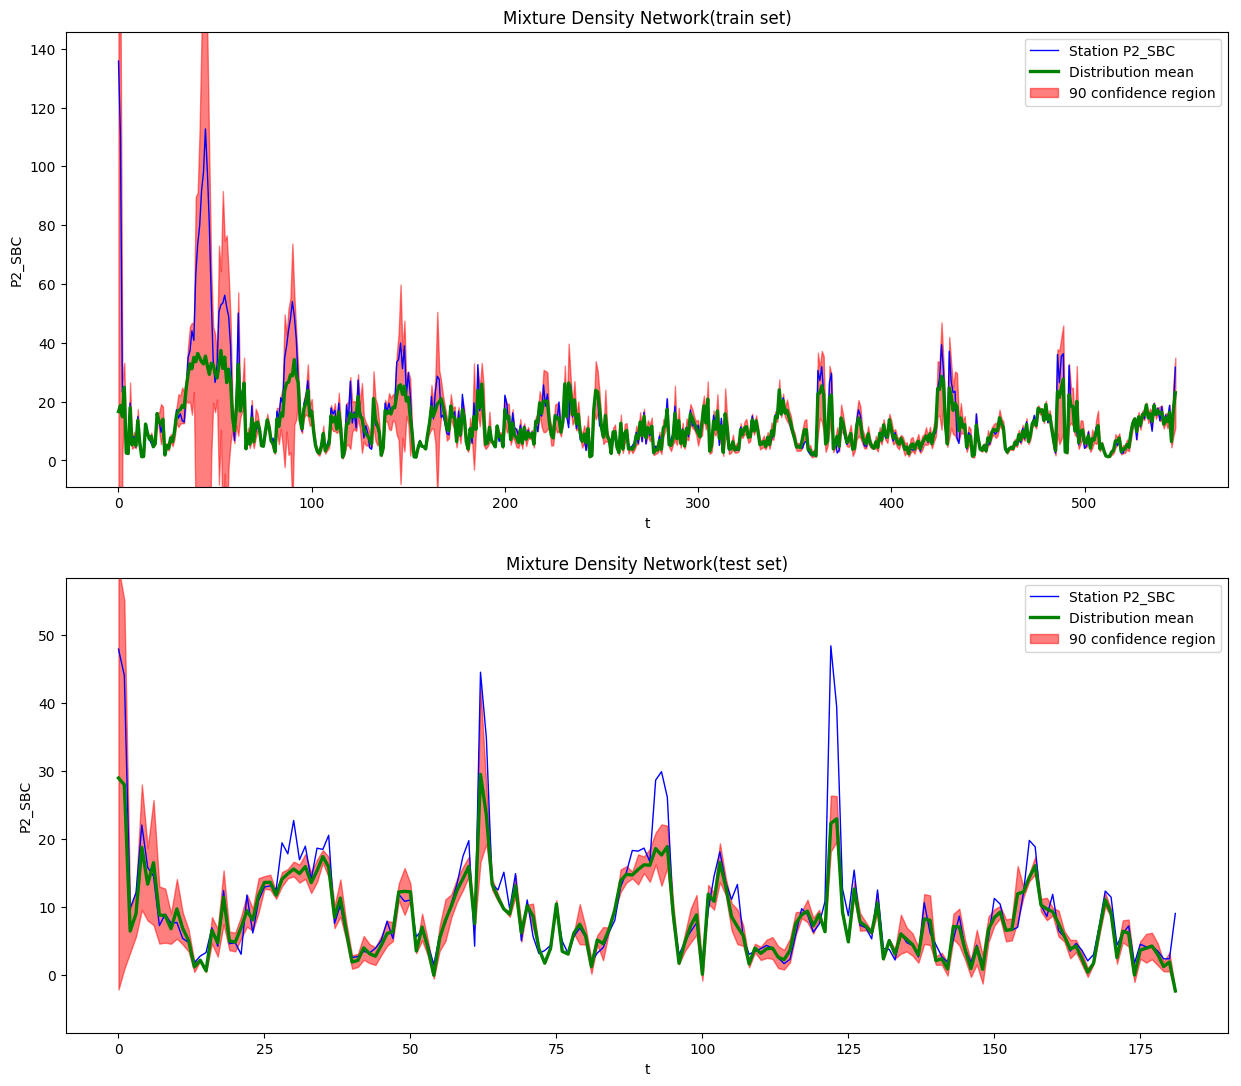
\includegraphics[height=0.6\textwidth, width=0.9\textwidth]{figures/model_plots/mdn_12h}
        \caption[MDN twelve hours plot]{A MDN model with good performance trained on twelve hourly averaged data}\label{fig:mdn-plot-12h}
      \end{figure}
    \end{center}
    \begin{center}
      \begin{figure}[h!]
        \centering
        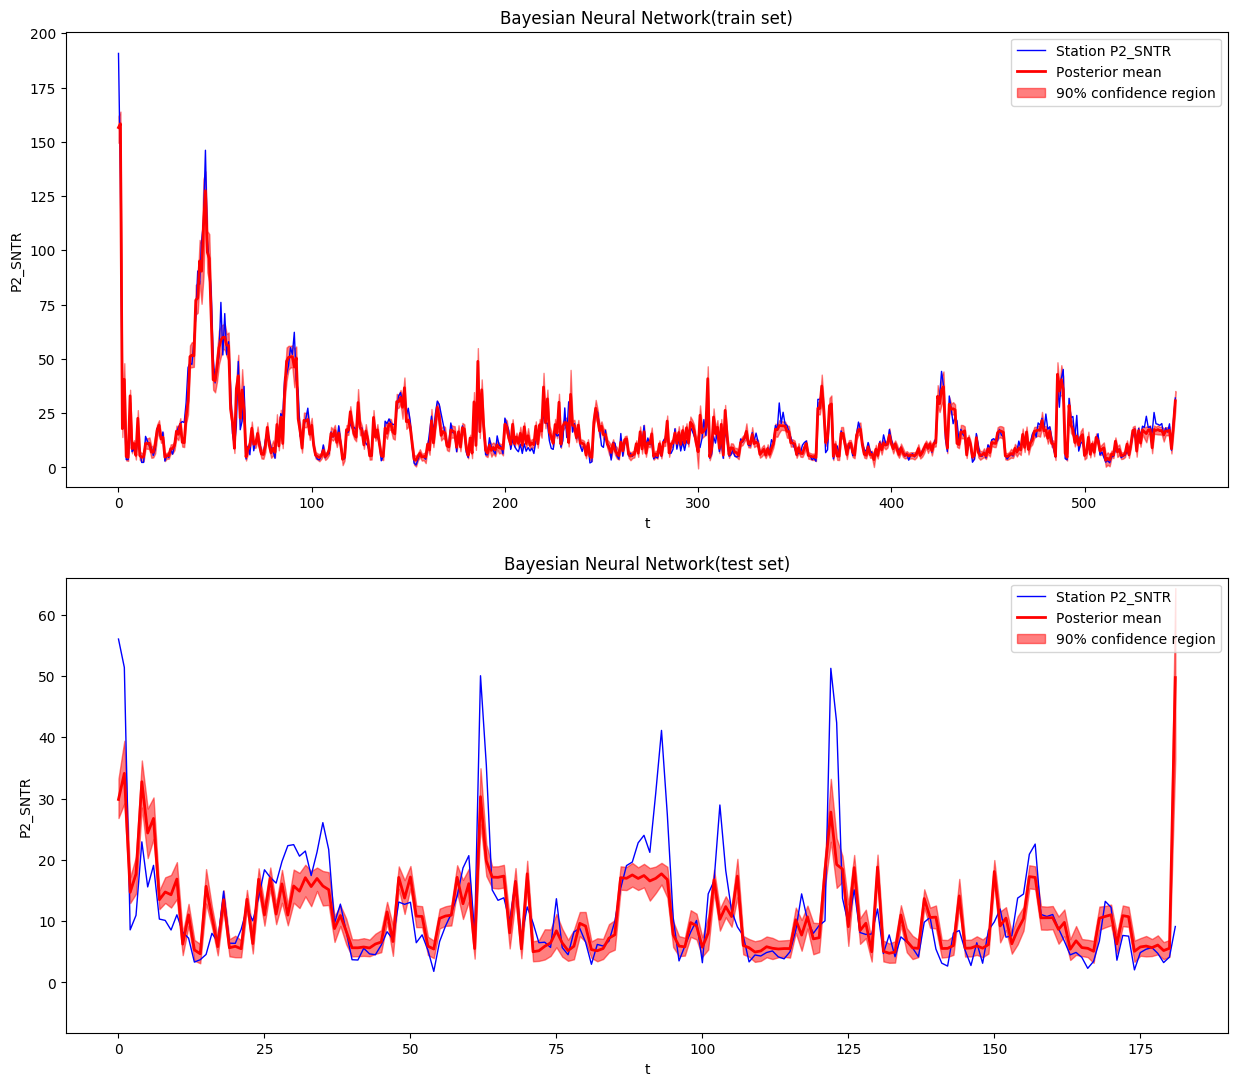
\includegraphics[height=0.6\textwidth, width=0.9\textwidth]{figures/model_plots/bnn_12h}
        \caption[BNN twelve hours plot]{A BNN model with good performance trained on twelve hourly averaged data}\label{fig:bnn-plot-12h}
      \end{figure}
    \end{center}
    \begin{center}
      \begin{figure}[h!]
        \centering
        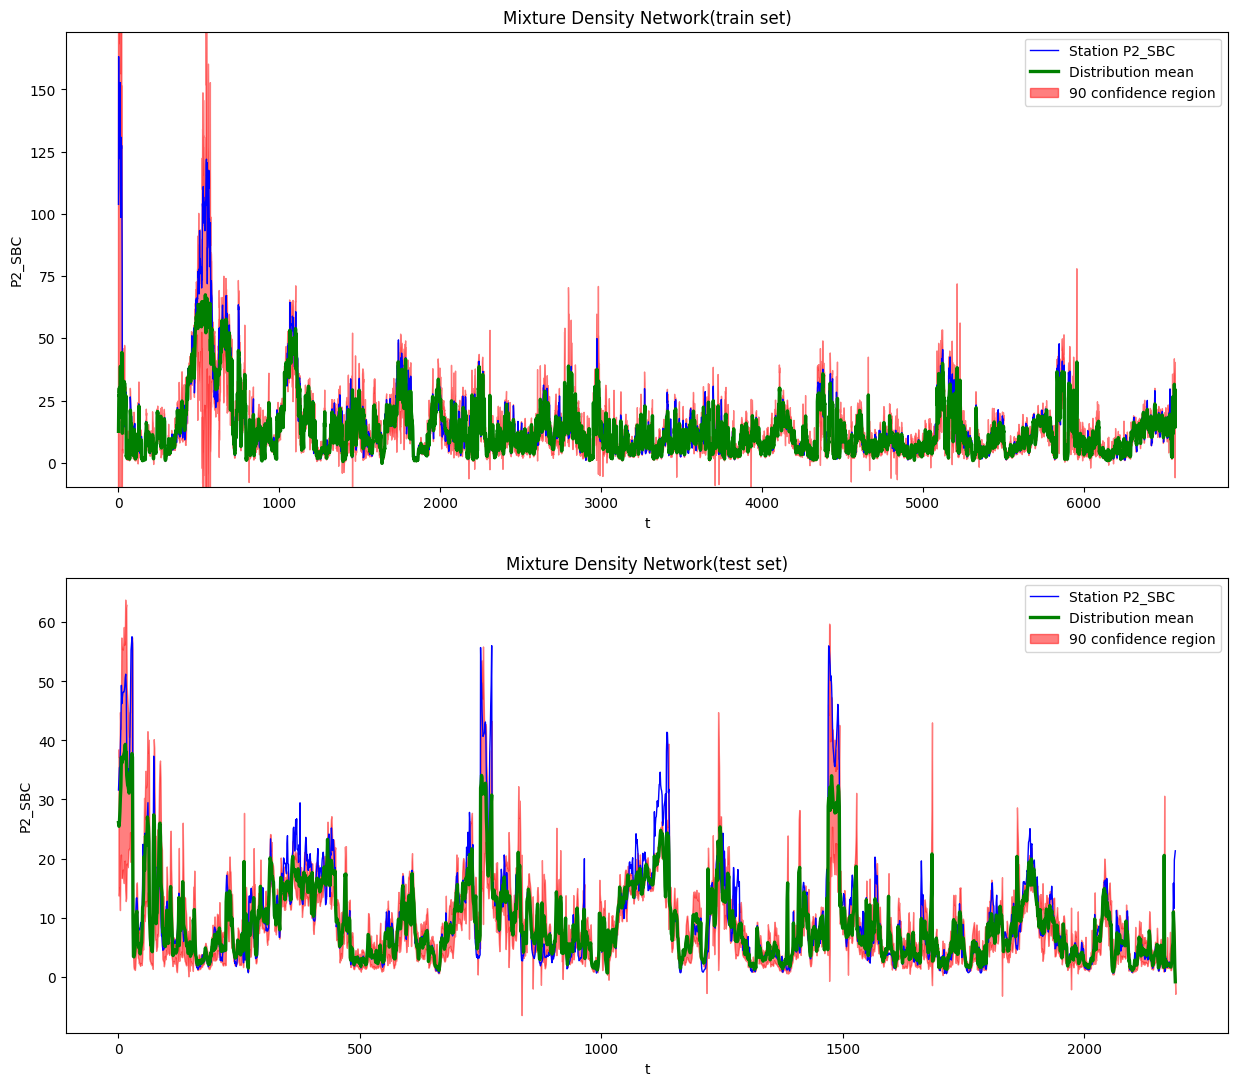
\includegraphics[height=0.6\textwidth, width=0.9\textwidth]{figures/model_plots/mdn_1h}
        \caption[MDN one hour plot]{A MDN model with good performance trained on one hourly averaged data}\label{fig:mdn-plot-1h}
      \end{figure}
    \end{center} 
    \begin{center}
      \begin{figure}[htpb]
        \centering
        \includegraphics[height=0.6\textwidth, width=0.9\textwidth]{figures/model_plots/bnn_1h}
        \caption[BNN one hour plot]{A BNN model with good performance trained on one hourly averaged data. To note is, however, that even though this BNN is considered to have good performance, BNNs struggled to predict the data in the context of one hour average. This plot illustrates this.}\label{fig:bnn-plot-1h}
      \end{figure}
    \end{center}
    \vfill
    \clearpage
    \chapter{Models rank histograms}\label{app:g}
    In this appendix we present the rank histograms of some of the models. As discussed in \refsec{sec:eval-model}, the rank histograms given here are representative of the rest and illustrate one of the problems of the built models. From all given rank histograms we can see that they are \texttt{U}-shaped which means that the models often miss the actual observation they are trying to predict.
    
    We give one histogram for the BNNs and MDNs per averaging period. \reffig{fig:rank-1d} illustrates the rank histograms of models trained with daily averaged data, \reffig{fig:rank-12h} -- models trained with twelve hourly averaged data and finally \reffig{fig:rank-1h} -- models trained with hourly averaged data. All of the histograms are calculated on the test set.
    
    \begin{figure}[h!]
      \centering
      \begin{subfigure}[t]{0.49\textwidth}
        \includegraphics[width=\textwidth,height=0.7\textwidth]{figures/model_plots/mdn-rank-1d}%
        \caption{A rank histogram of a MDN model trained with daily averaged data.}
      \end{subfigure}
      %%%%%%%%%%%%%%%%%%%%%%%%%%%%%%%%%%%%%%%%%%%%%%%%%%% 
      \begin{subfigure}[t]{0.49\textwidth}
        \includegraphics[width=\textwidth,height=0.7\textwidth]{figures/model_plots/bnn-rank-1d}%
        \caption{A rank histogram of a BNN model trained with daily averaged data.}
      \end{subfigure}
      \caption[Rank histograms (daily averaged data)]{}\label{fig:rank-1d}
    \end{figure}
    \begin{figure}[h!]
      \centering
      \begin{subfigure}[t]{0.49\textwidth}
        \includegraphics[width=\textwidth,height=0.7\textwidth]{figures/model_plots/mdn-rank-12h}%
        \caption{A rank histogram of a MDN model trained with daily averaged data.}
      \end{subfigure}
      %%%%%%%%%%%%%%%%%%%%%%%%%%%%%%%%%%%%%%%%%%%%%%%%%%% 
      \begin{subfigure}[t]{0.49\textwidth}
        \includegraphics[width=\textwidth,height=0.7\textwidth]{figures/model_plots/bnn-rank-12h}%
        \caption{A rank histogram of a BNN model trained with twelve hourly averaged data.}
      \end{subfigure}
      \caption[Rank histograms (twelve hourly averaged data)]{}\label{fig:rank-12h}
    \end{figure}
    \begin{figure}[H]
      \centering
      \begin{subfigure}[t]{0.49\textwidth}
        \includegraphics[width=\textwidth,height=0.7\textwidth]{figures/model_plots/mdn-rank-1h}%
        \caption{A rank histogram of a MDN model trained with averaged data.}
      \end{subfigure}
      %%%%%%%%%%%%%%%%%%%%%%%%%%%%%%%%%%%%%%%%%%%%%%%%%%% 
      \begin{subfigure}[t]{0.49\textwidth}
        \includegraphics[width=\textwidth,height=0.7\textwidth]{figures/model_plots/bnn-rank-1h}%
        \caption{A rank histogram of a BNN model trained with hourly averaged data.}
      \end{subfigure}
      \caption[Rank histograms (hourly averaged data)]{}\label{fig:rank-1h}
    \end{figure}
    \vfill
    \clearpage
    \chapter{Empirical models plots}\label{app:h}
    In this appendix we give plots of the predictions made by the empirical models. As these models do not make difference between test and train set, we have evaluated them only on the part of the data that would have been used as a test set for a MDN or a BNN.

    \begin{center}
      \begin{figure}[h!]
        \centering
        \includegraphics[height=0.5\textwidth, width=0.9\textwidth]{figures/model_plots/emp-1d}
        \caption[Empirical one day plot]{An empirical model predicting daily averaged data.}\label{fig:emp-1d}
      \end{figure}
    \end{center}
    \begin{center}
      \begin{figure}[h!]
        \centering
        \includegraphics[height=0.5\textwidth, width=0.9\textwidth]{figures/model_plots/emp-12h}
        \caption[Empirical twelve hour plot]{An empirical model predicting twelve hourly averaged data.}\label{fig:emp-12h}
      \end{figure}
    \end{center}
    \begin{center}
      \begin{figure}[H]
        \centering
        \includegraphics[height=0.5\textwidth, width=0.9\textwidth]{figures/model_plots/emp-12h}
        \caption[Empirical one hour plot]{An empirical model predicting hourly averaged data.}\label{fig:emp-1h}
      \end{figure}
    \end{center}
  \end{appendices}
  \clearpage
  \addcontentsline{toc}{section}{References}
  \bibliographystyle{alpha}
  \bibliography{references}
\end{interlude}
\end{document}